\chapter{Setup Implementation}
\label{chap:implementation}

\section{Overview}

As stated before, C-RAN is still in development and it is not already a solid
standard, so exploring setups and their feasibility is very interesting to
increase the ways to implement this new standard in countries which does not
have a very good infrastructure.

The first setup thought was using the ML605 FMC LPC connector and the FMComms2,
this setup was very important because in it was possible to understand how to
integrate the board design with the need of the project. Then the device was
moved to the FMC HPC connector and the design with the ML605 was finished.

After getting the experience with ML605 and ISE design tools, it was time to use
a more updated board and design tool, thus the idea of porting the initial
design from ML605 to the VC707 board came. Since ISE has no support for VC707
and is a software with its development halted, going to the most updated tool
from Xilinx is natural, so the second setup is using vivado design tools and
VC707 with FMC HPC connector and FMComms2.

Another thing to give attention is that with ISE the design flow was more manual
and if there was the need to rebuild a project almost from the scratch, just
with the HDL source files, the other necessary ips should be created and
configured again, which took a lot of time, but with Vivado the block diagram
design flow and the .tcl scripts became more popular, they existed in ISE
however they were not popular. With the TCL scripts it is possible to create
project, import files, instantiate and configure both user and default IPs, as
well as run synthesis, implementation and generate bitstream steps, which saves
a lot of time in development.

%figura das duas fases do SETUP downlink e Uplink

%tx block diagram
\begin{figure}[htbp]
    \centering
    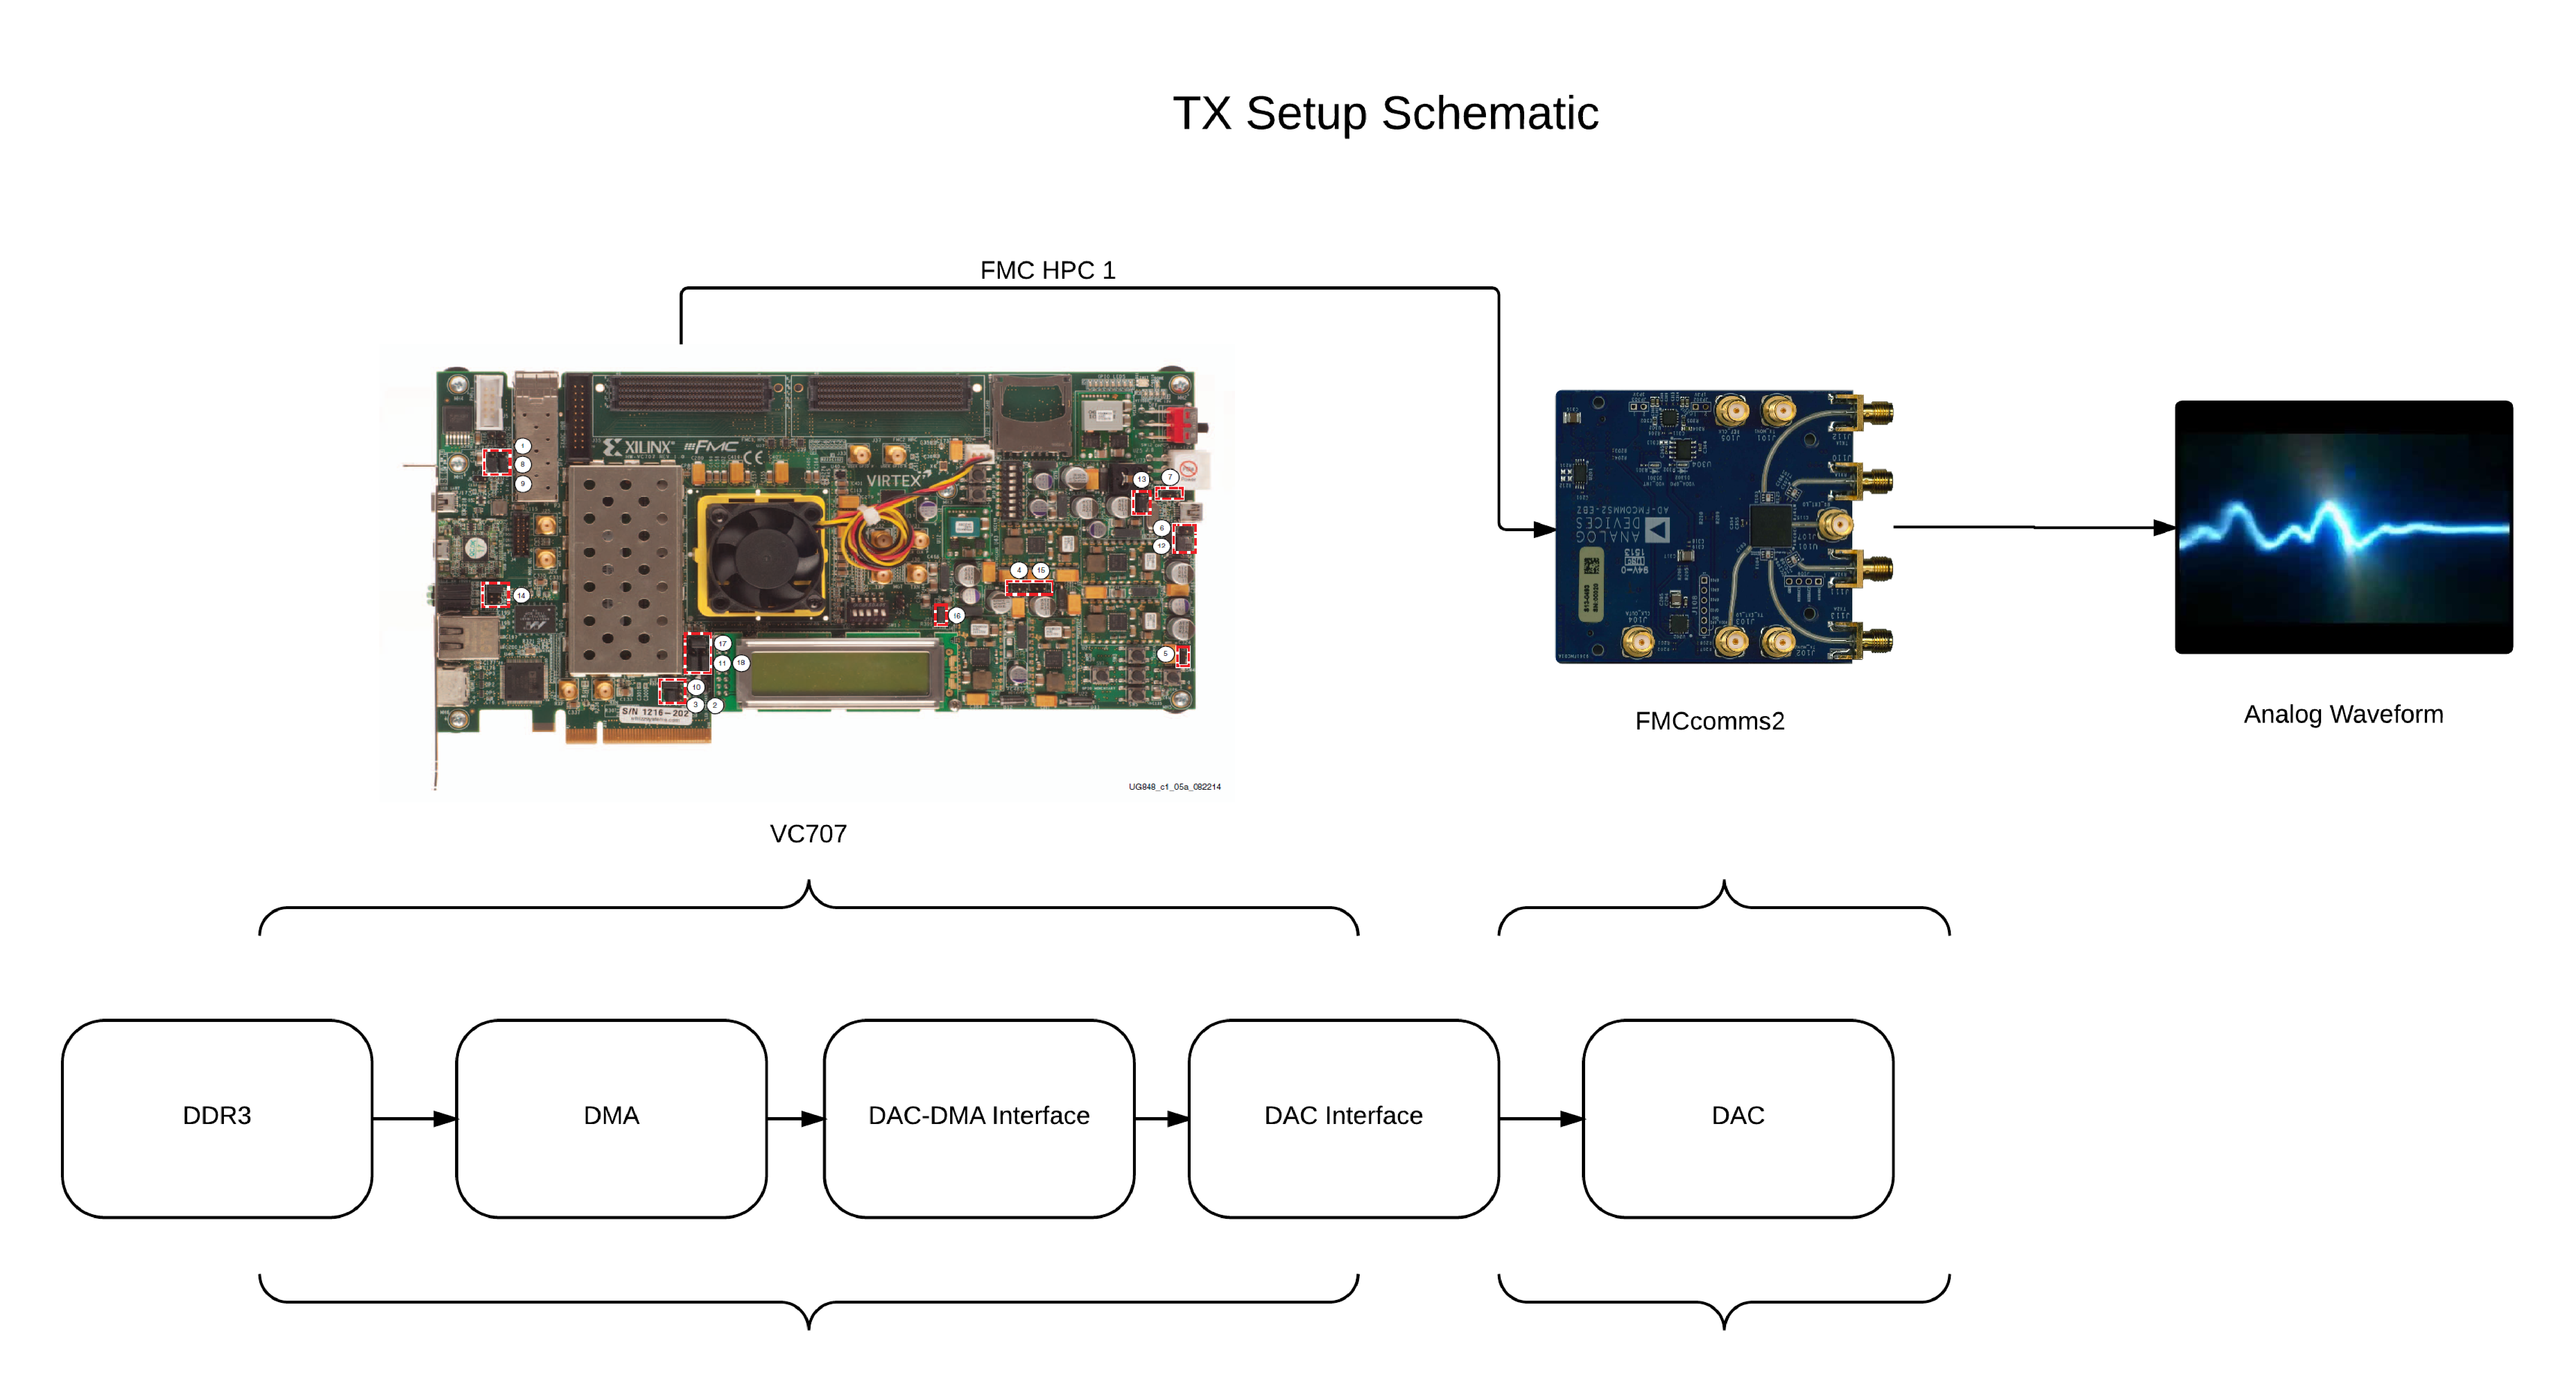
\includegraphics[width=0.65\textwidth]{./figures/tx_setup}
    \caption{ Transmitter Setup Block Diagram
    \label{fig:txsetup}}
\end{figure}

%rx block diagram
\begin{figure}[htbp]
    \centering
    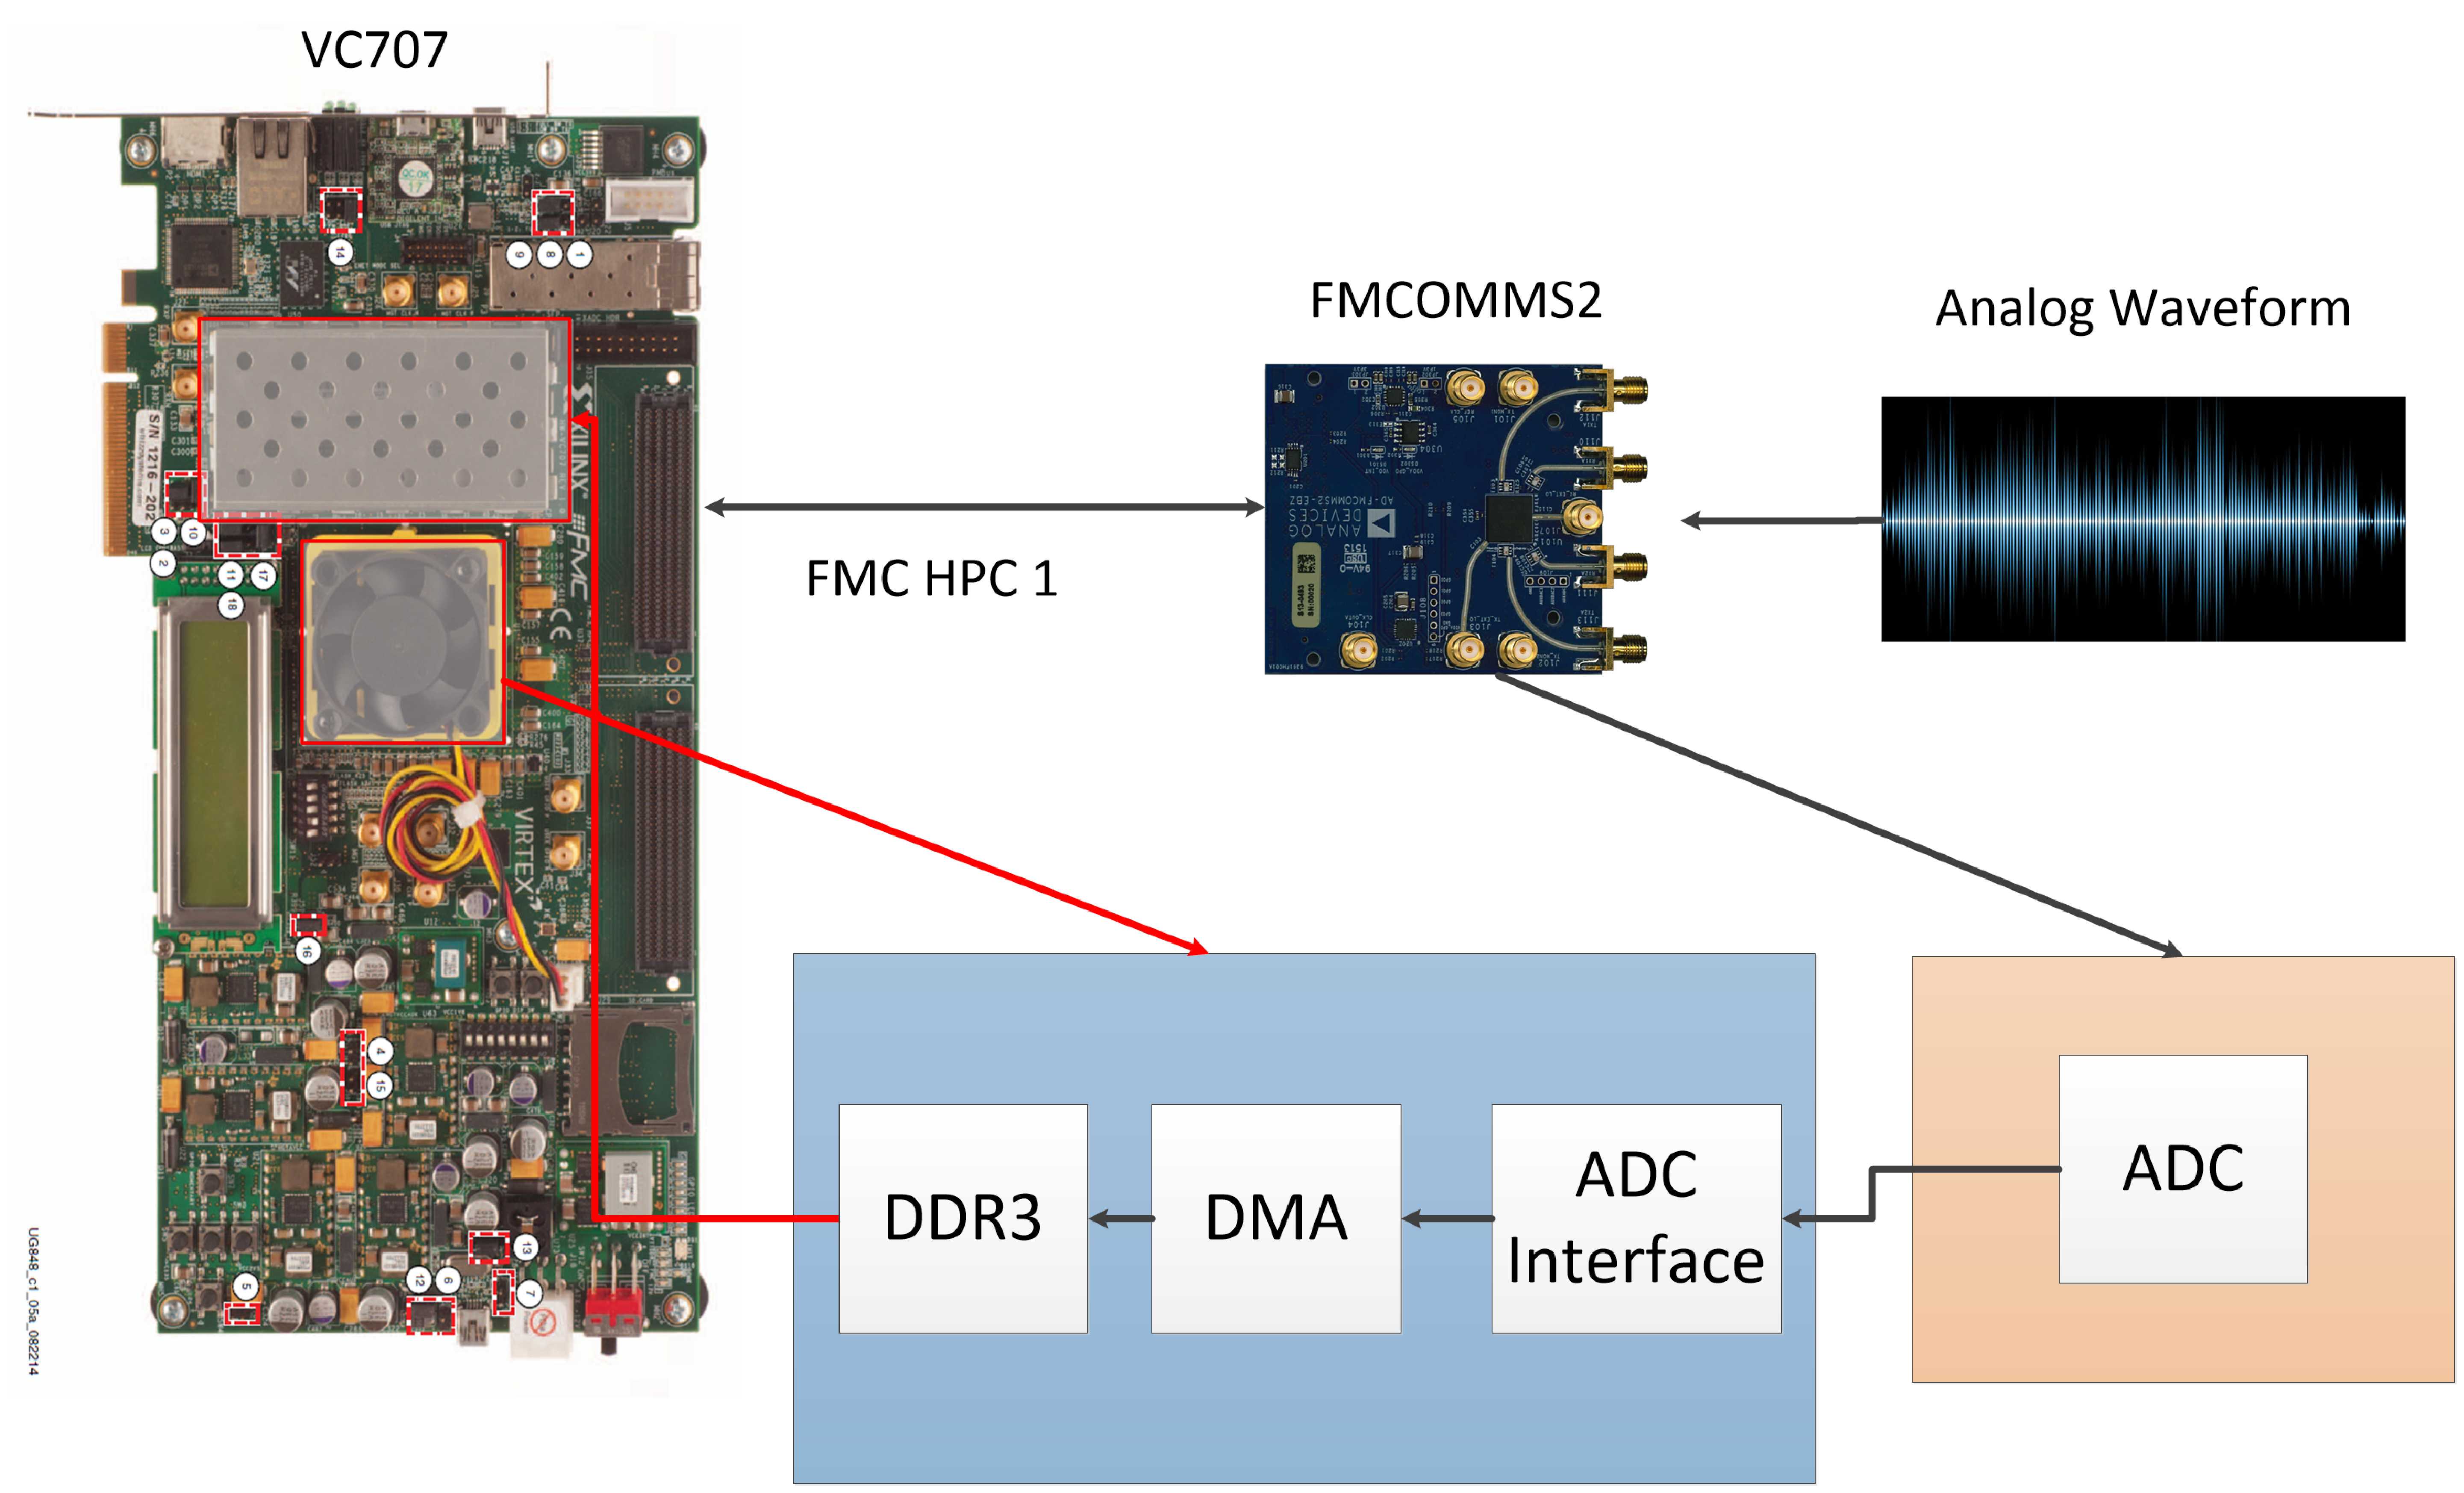
\includegraphics[width=0.65\textwidth]{./figures/rx_setup}
    \caption{ Receiver Setup Block Diagram
    \label{fig:rxsetup}}
\end{figure}

%--------------------------------------------FPGA-----------------------------------------
\section{FPGA}

FPGA stands for Field Programmable Gate Array, which are digital integrated
circuits (IC) that contain configurable (programmable) blocks of logic along
with configurable interconnects between these blocks. Design engineers can
configure (program) such devices to perform a wide variety of tasks. Depending
on the way in which they are built, some FPGA boards may only be programmed a
single time (OTP - One time Programmable), like the EPROM memory, while others
may be reprogrammed over and over again, which is the case of the FPGA boards
used in this work.\cite{max2004}

The “field programmable” portion of the FPGA’s name refers to the fact that its
programming takes place “in the field” (as opposed to devices whose internal
functionality is hard-wired by the manufacturer). This mean that FPGAs
connections are electrically activated and deactivated, thus the fpga can be
programmed in the factory or by the developer, when a  FPGA designed is
implemented in a hardwired circuit it is called ASIC (Application Specific
Integrated Circuit).

The FPGAs are so flexible and interesting to work with that there is a field of
study in the computer engineering/science which studies them, the reconfigurable
computing field.

This work was implemented in two FPGAs the Virtex 6 and Virtex 7, thus
implemented in two different development boards, the ML605 (Virtex 6) and the
VC707 (Virtex 7), there is also support for the VC709 board. However not fully
functional.This section aims to describe briefly the boards and Tools used in
this work.


\subsection{ML605 - Virtex6}
This board was used in the first version of the setup, still it lacked better
clock sources and dividers, it was also older the the VC707, thus the design was
ported to VC707, below there is a list of the features of the ML605 development
board.

In the figure \ref{fig:ml605} there is a picture of the board and in the figure
\ref{fig:ml605bd} there is also a functional block diagram of the board, this
information was acquired in the official board manual \cite{xilinx:ml605}.


\textbf{ML605 Evaluation Module Features:}
\begin{enumerate}
  \item Virtex-6 XC6VLX240T-1FFG1156 FPGA
  \item 512 MB DDR3 Memory SODIMM
  \item 128 Mb Platform Flash XL
  \item 32 MB Linear BPI Flash
  \item System ACE CF and CompactFlash Connector
  \item USB JTAG
  \item Clock Generation
  \begin{itemize}
    \item Fixed 200 MHz oscillator (differential)
    \item Socketed 2.5V oscillator (single-ended)
    \item SMA connectors (differential)
    \item SMA connectors for MGT clocking
  \end{itemize}

  \item Multi-Gigabit Transceivers (GTX MGTs)

  \begin{itemize}
    \item FMC - HPC connector
    \item FMC - LPC connector
    \item SMA
    \item PCIe
    \item SFP Module connector
    \item Ethernet PHY SGMII interface
  \end{itemize}

  \item PCI Express Endpoint Connectivity

  \begin{itemize}
    \item Gen1 8-lane (x8)
    \item Gen2 4-lane (x4)
  \end{itemize}

  \item SFP Module Connector
  \item 10/100/1000 Tri-Speed Ethernet PHY
  \item USB-to-UART Bridge
  \item USB Controller
  \item DVI Codec
  \item IIC Bus

  \begin{itemize}
    \item IIC EEPROM - 1 KB
    \item DDR3 SODIMM socket
    \item DVI CODEC
    \item DVI connector
    \item FMC HPC connector
    \item FMC LPC connector
    \item SFP module connector
  \end{itemize}

  \item Status LEDs

  \begin{itemize}
    \item Ethernet status
    \item FPGA INIT
    \item FPGA DONE
    \item System ACE CF Status
  \end{itemize}
  \item User I/O

  \begin{itemize}
    \item USER LED Group 1 - GPIO (8)
    \item USER LED Group 2 - directional (5)
    \item User pushbuttons - directional (5)
    \item CPU reset pushbutton
    \item User DIP switch - GPIO (8-pole)
    \item User SMA GPIO connectors (2)
    \item LCD character display (16 characters x 2 lines)
  \end{itemize}

  \item Switches
  \begin{itemize}
    \item Power on/off slide switch
    \item System ACE CF reset pushbutton
    \item System ACE CF bitstream image select DIP switch
    \item Configuration MODE DIP switch
  \end{itemize}

  \item VITA 57.1 FMC HPC Connector
  \item VITA 57.1 FMC LPC Connector
  \item Power Management

  \begin{itemize}
    \item PMBus voltage and current monitoring via TI power controller
  \end{itemize}

  \item System Monitor
  \item Configuration Options
  \begin{enumerate}
    \item 128 Mb Platform Flash XL
    \item 32 MB Linear BPI Flash
    \item System ACE CF and CompactFlash Connector
    \item USB JTAG
  \end{enumerate}

\end{enumerate}

%ml605 board
\begin{figure}[htbp]
    \centering
    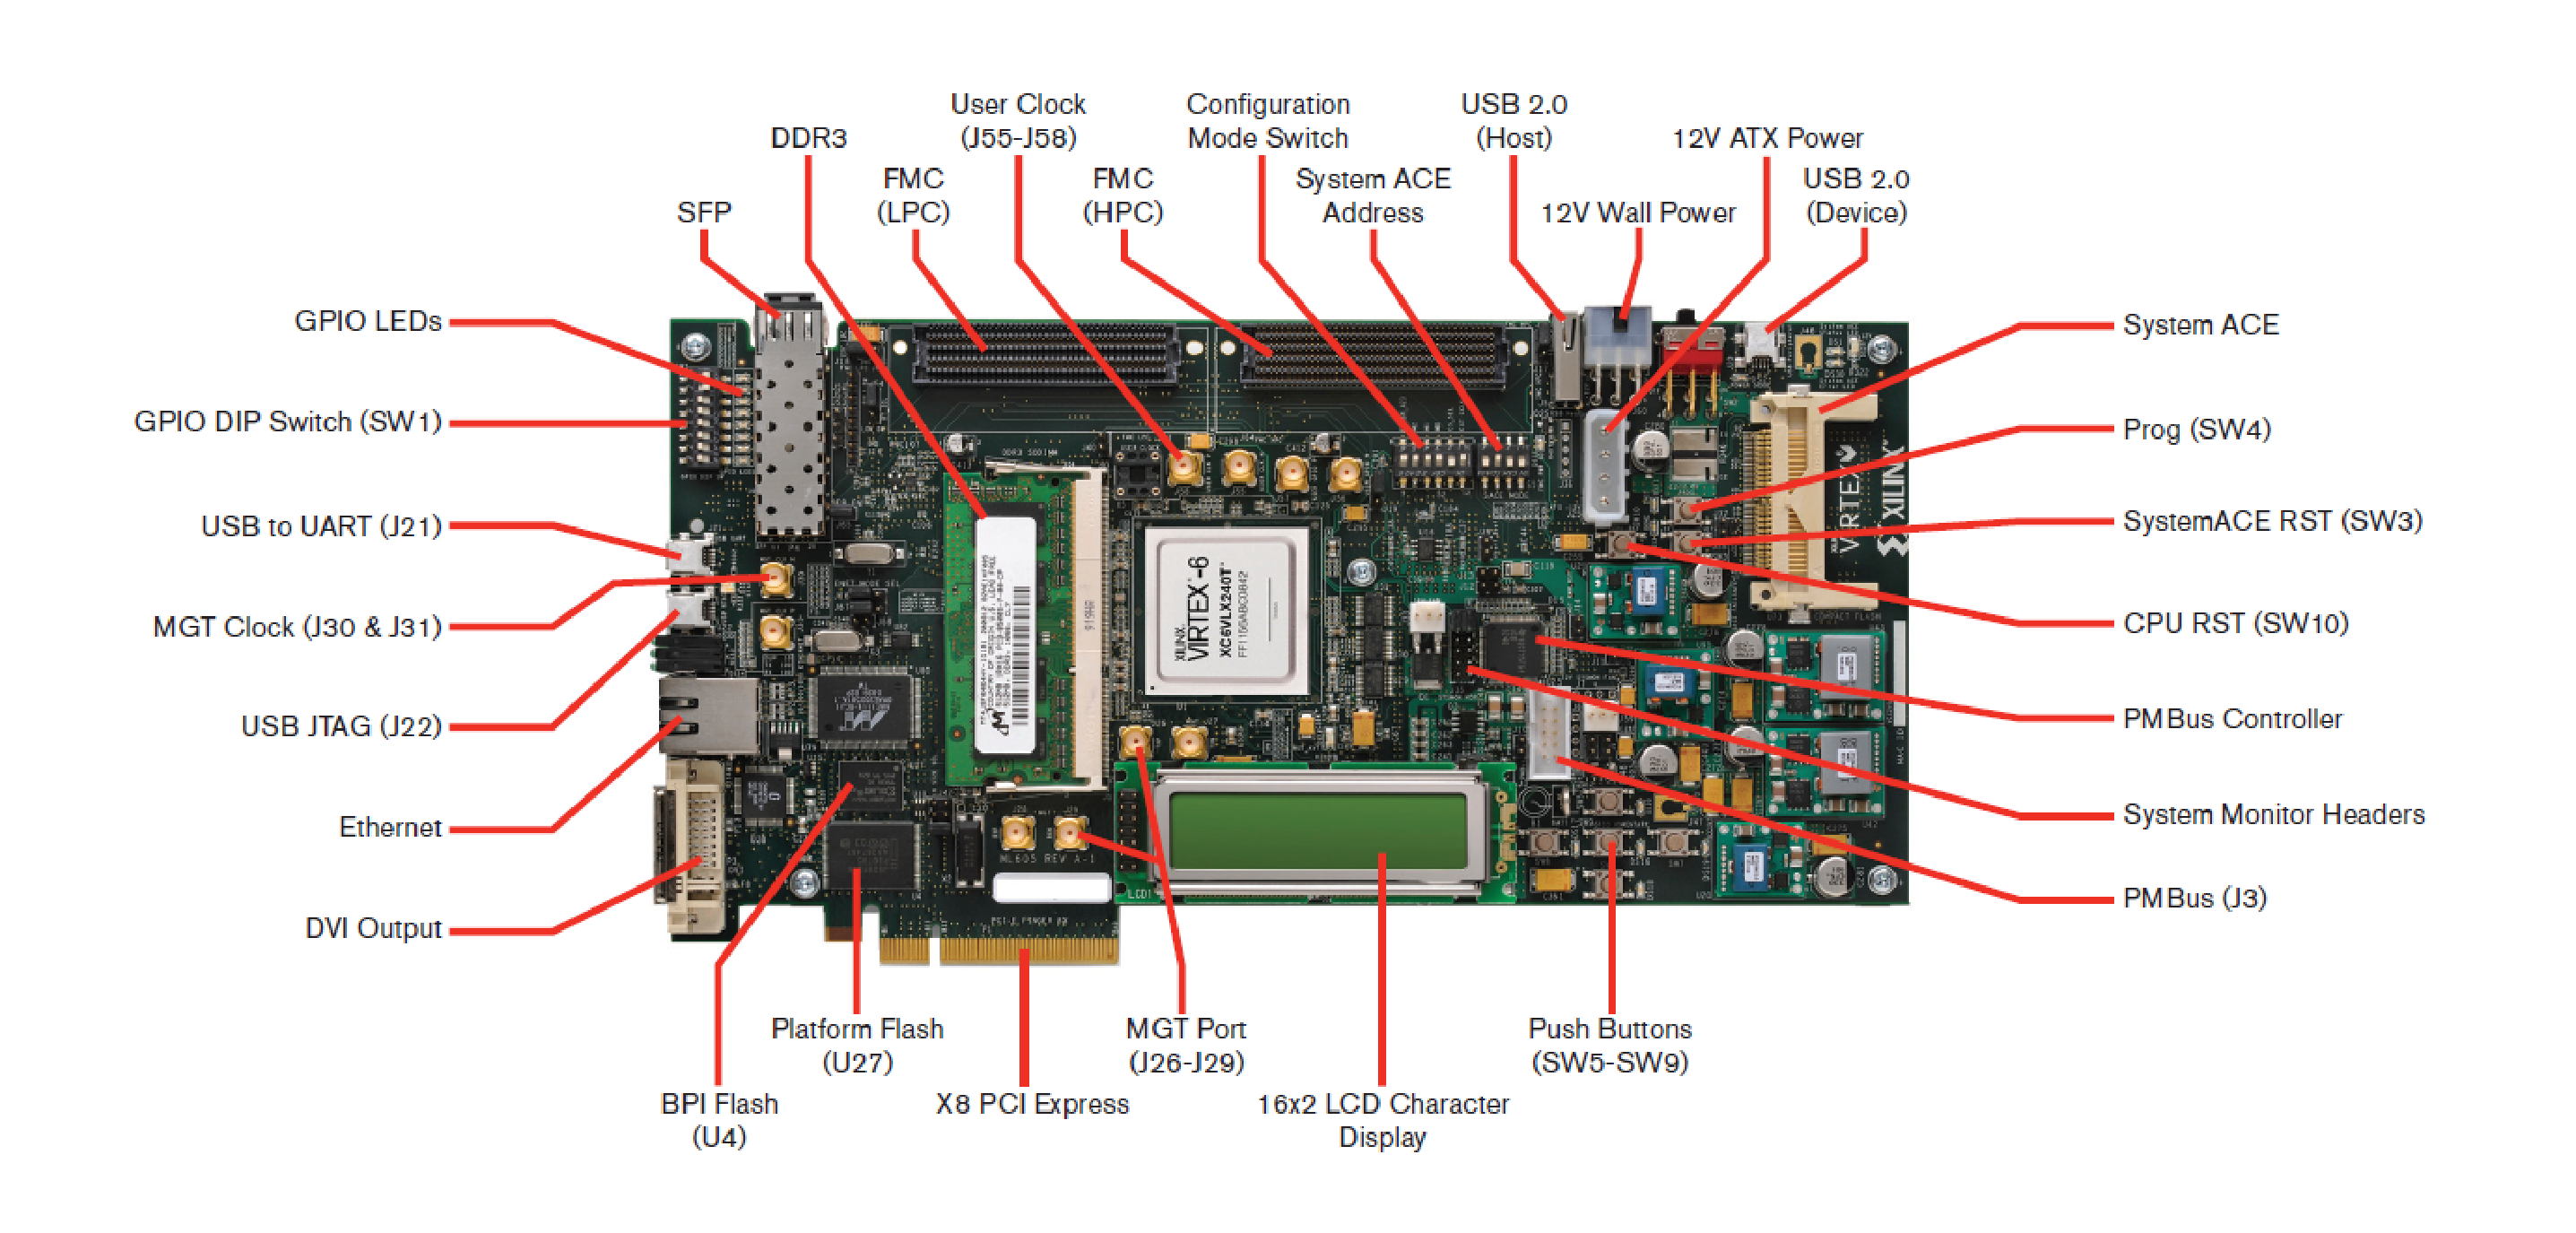
\includegraphics[width=0.85\textwidth]{./figures/ml605}
    \caption{ ML605 Development Board
    \label{fig:ml605}}
\end{figure}
\clearpage

%ml605 block diagram
\begin{figure}[htbp]
    \centering
    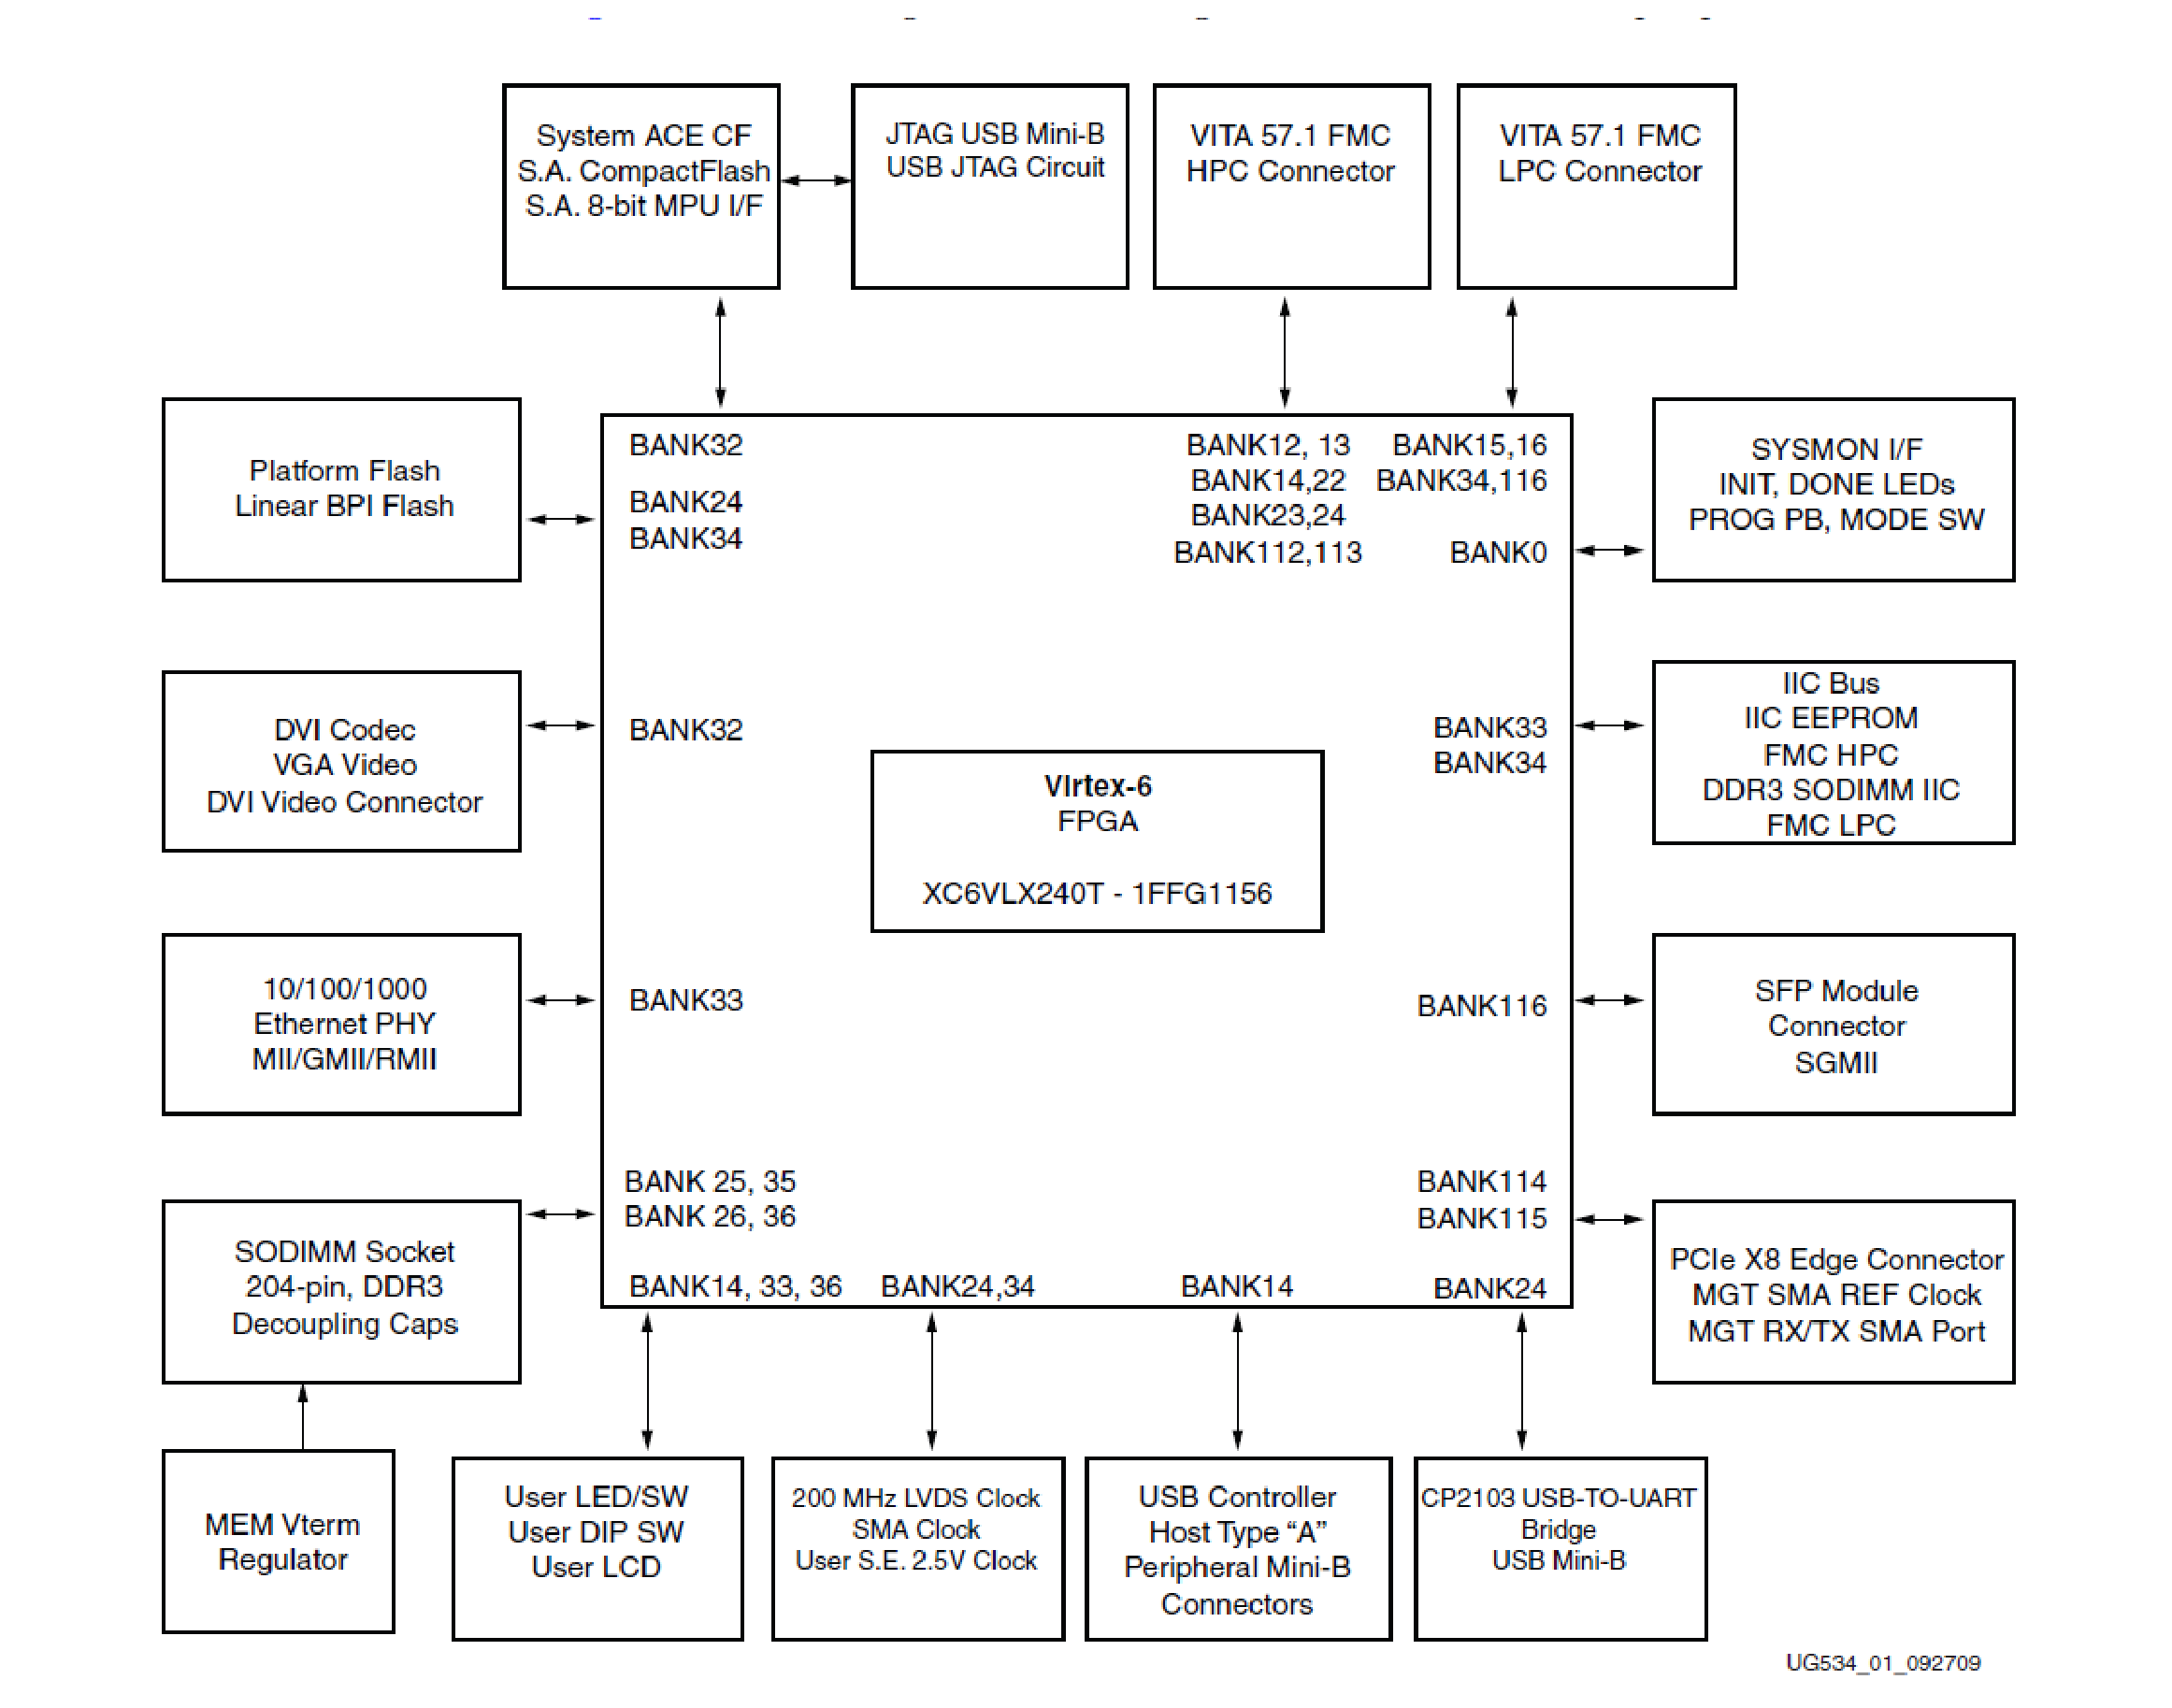
\includegraphics[width=0.55\textwidth]{./figures/ml605_bd}
    \caption{ ML605 Functional Block Diagram
    \label{fig:ml605bd}}
\end{figure}

\subsection{VC707 - Virtex7}

The final results of this setup were generated in the VC707 board
\cite{xilinx:vc707}, because it has a possibility of expansion and has better
clock generation and treatment options compared to the ML605 board.

\textbf{VC707 Evaluation Board Features}

\begin{enumerate}

  \item Virtex-7 XC7VX485T-2FFG1761C FPGA
  \item 1 GB DDR3 memory SODIMM
  \item 128 MB Linear byte peripheral interface (BPI) Flash memory
  \item USB 2.0 ULPI Transceiver
  \item Secure Digital (SD) connector
  \item USB JTAG through Digilent module
  \item Clock Generation

  \begin{itemize}
    \item Fixed 200 MHz LVDS oscillator (differential)
    \item IIC programmable LVDS oscillator (differential)
    \item SMA connectors (differential)
    \item SMA connectors for GTX transceiver clocking
  \end{itemize}

  \item GTX transceivers

  \begin{itemize}
    \item FMC1 HPC connector (eight GTX transceivers)
    \item FMC2 HPC connector (eight GTX transceiver)
    \item SMA connectors (one pair each for TX, RX, and REFCLK)
    \item PCI Express (eight lanes)
    \item Small form-factor pluggable plus (SFP+) connector
    \item Ethernet PHY SGMII interface (RJ-45 connector)
  \end{itemize}

  \item PCI Express endpoint connectivity

  \begin{itemize}
    \item Gen1 8-lane (x8)
    \item Gen2 8-lane (x8)
  \end{itemize}

  \item SFP+ Connector
  \item 10/100/1000 tri-speed Ethernet PHY
  \item USB-to-UART bridge
  \item HDMI codec
  \item I2C bus

  \begin{itemize}
    \item IIC MUX
    \item IIC EEPROM (1 KB)
    \item USER I2C programmable LVDS oscillator
    \item DDR3 SODIMM socket
    \item HDMI codec
    \item FMC1 HPC connector
    \item FMC2 HPC connector
    \item SFP+ connector
    \item IIC programmable jitter-attenuating precision clock multiplier
  \end{itemize}

  \item Status LEDs

  \begin{itemize}
    \item Ethernet status
    \item Power good
    \item FPGA INIT
    \item FPGA DONE
  \end{itemize}

  \item User I/O
  \begin{itemize}
    \item User LEDs (eight GPIO)
    \item User pushbuttons (five directional)
    \item CPU reset pushbutton
    \item User DIP switch (8-pole GPIO)
    \item User SMA GPIO connectors (one pair)
    \item LCD character display (16 characters x 2 lines)
  \end{itemize}

  \item Switches

  \begin{itemize}
    \item Power on/off slide switch
    \item FPGA\_PROB\_B pushbutton
    \item Configuration mode DIP switch
  \end{itemize}

  \item VITA 57.1 FMC1 HPC Connector
  \item VITA 57.1 FMC2 HPC Connector
  \item Power management

  \begin{itemize}
    \item PMBus voltage and current monitoring through TI power controller
  \end{itemize}

  \item XADC header
  \item Configuration options

  \begin{itemize}
    \item Linear BPI Flash memory
    \item USB JTAG configuration port
    \item Platform cable header JTAG configuration port
  \end{itemize}

\end{enumerate}

The characteristic which make this project be ported to the VC707 board is the
clock generation options that can be used to synchronize the FMComms2 and the FPGA
board in a future implementation.

In the figures \ref{fig:vc707} and
\ref{fig:vc707bd} there are the evaluation board picture and the high-level block
diagram respectively.

%vc707 board
\begin{figure}[htbp]
    \centering
    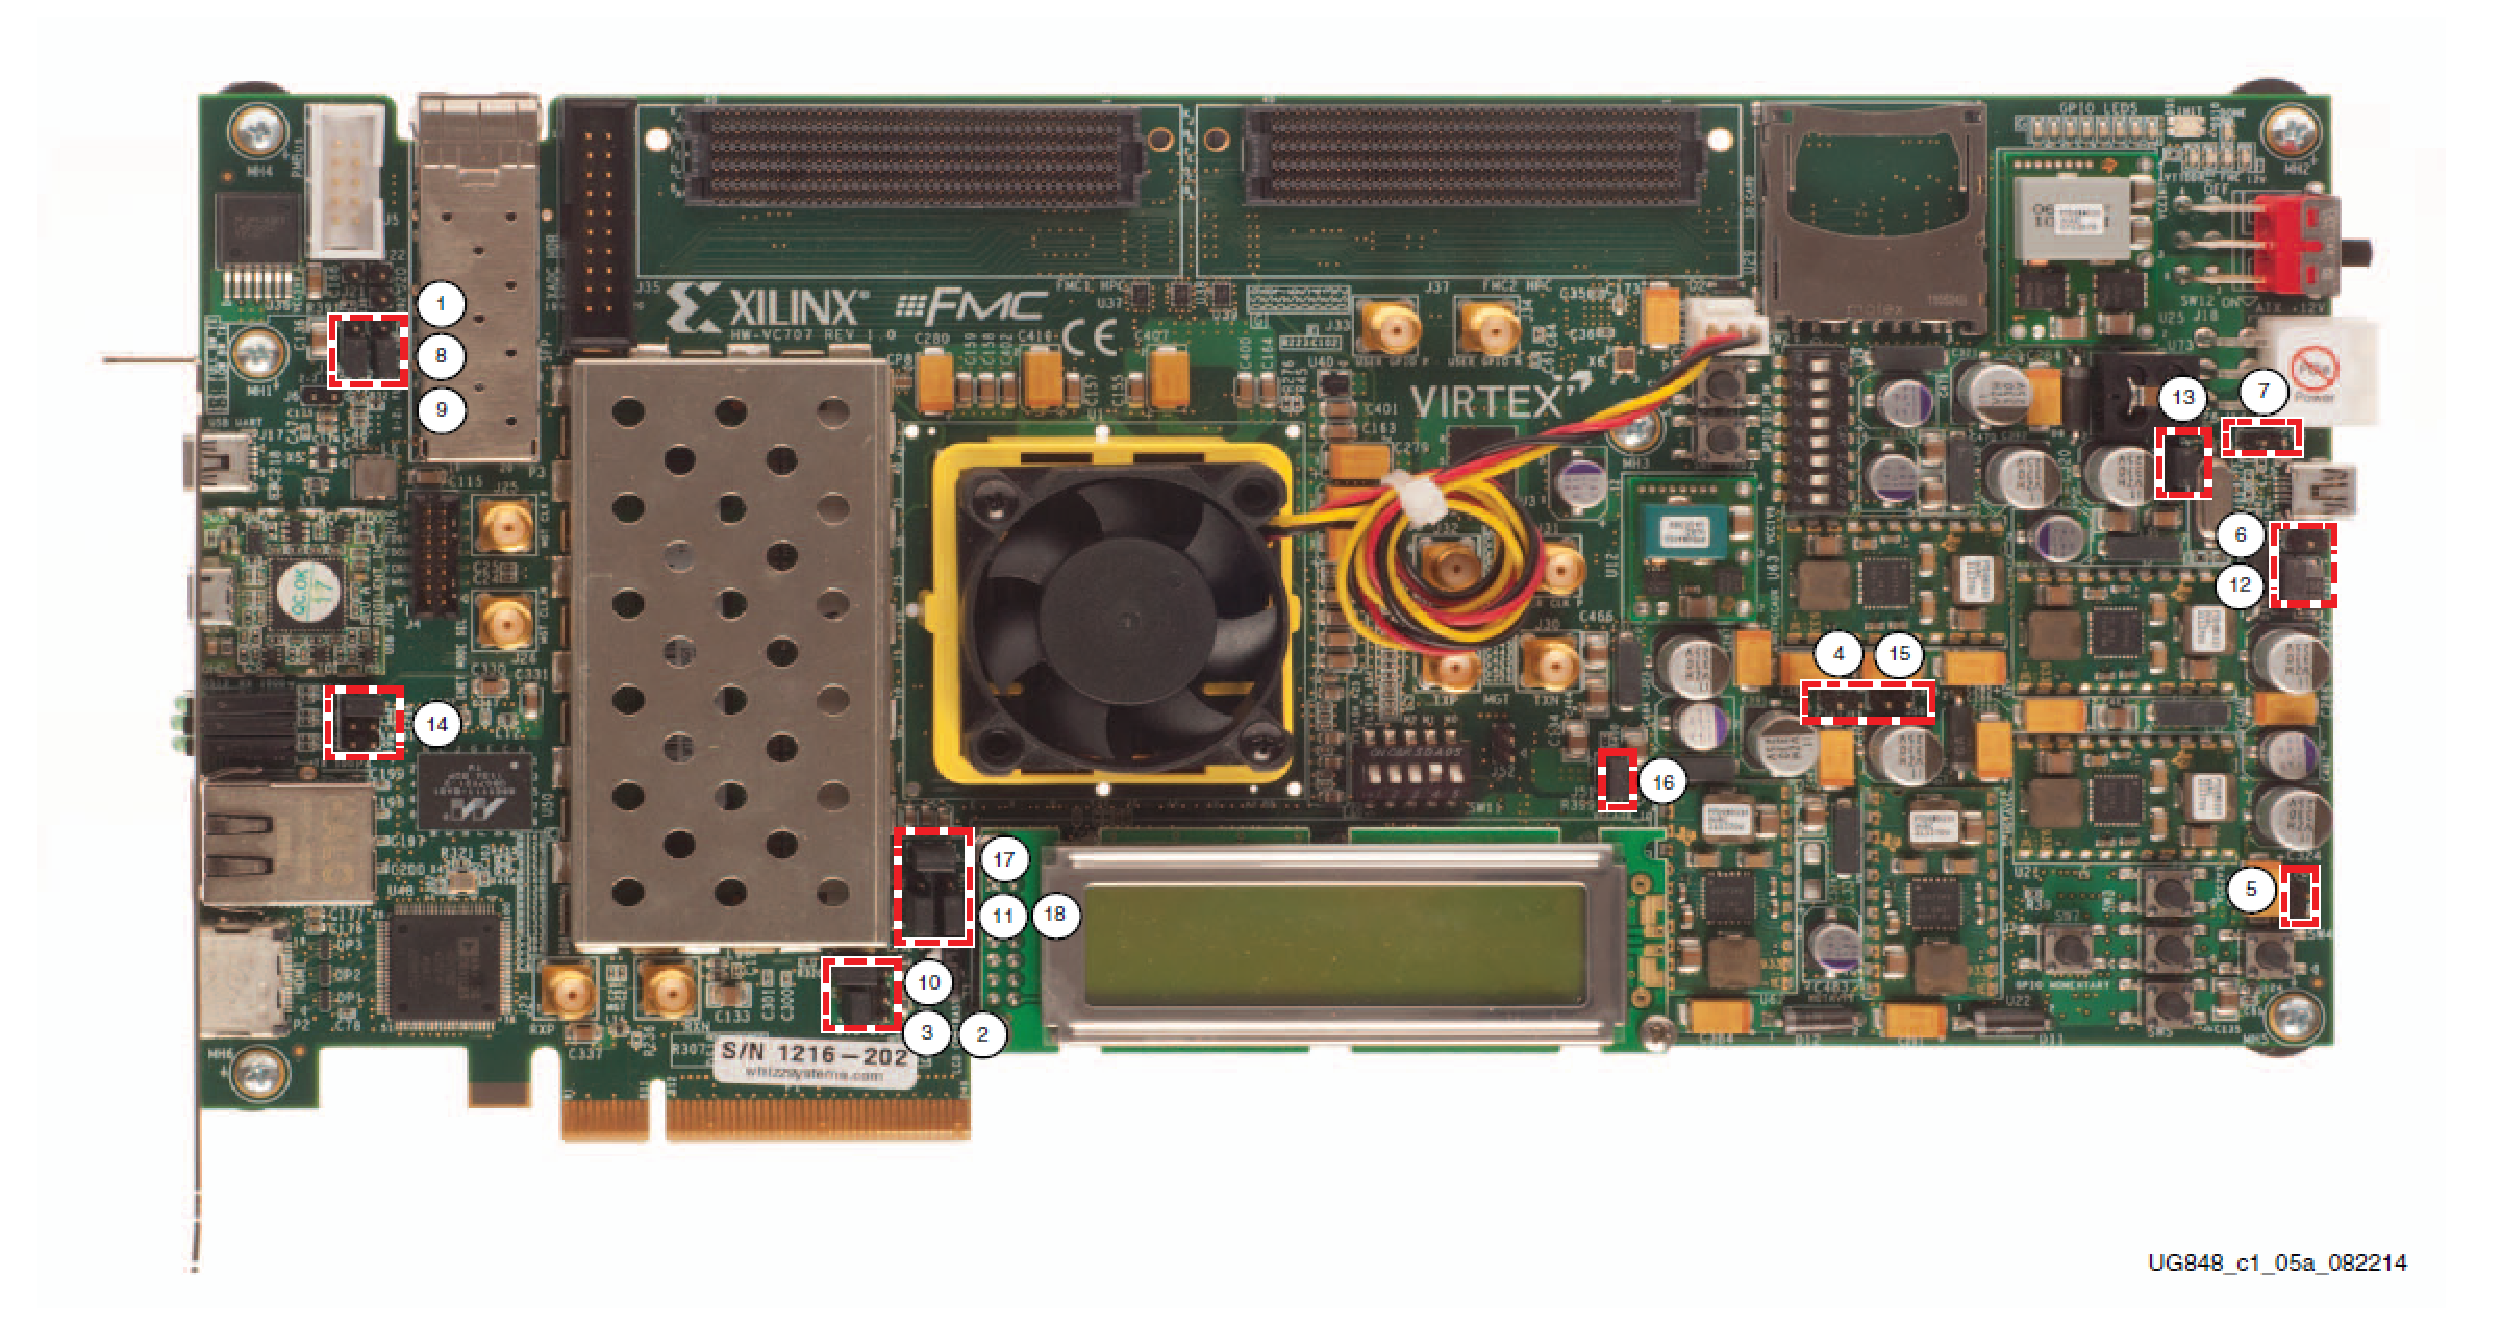
\includegraphics[width=0.65\textwidth]{./figures/vc707}
    \caption{ VC707 Development Board
    \label{fig:vc707}}
\end{figure}

%vc707 block diagram
\begin{figure}[htbp]
    \centering
    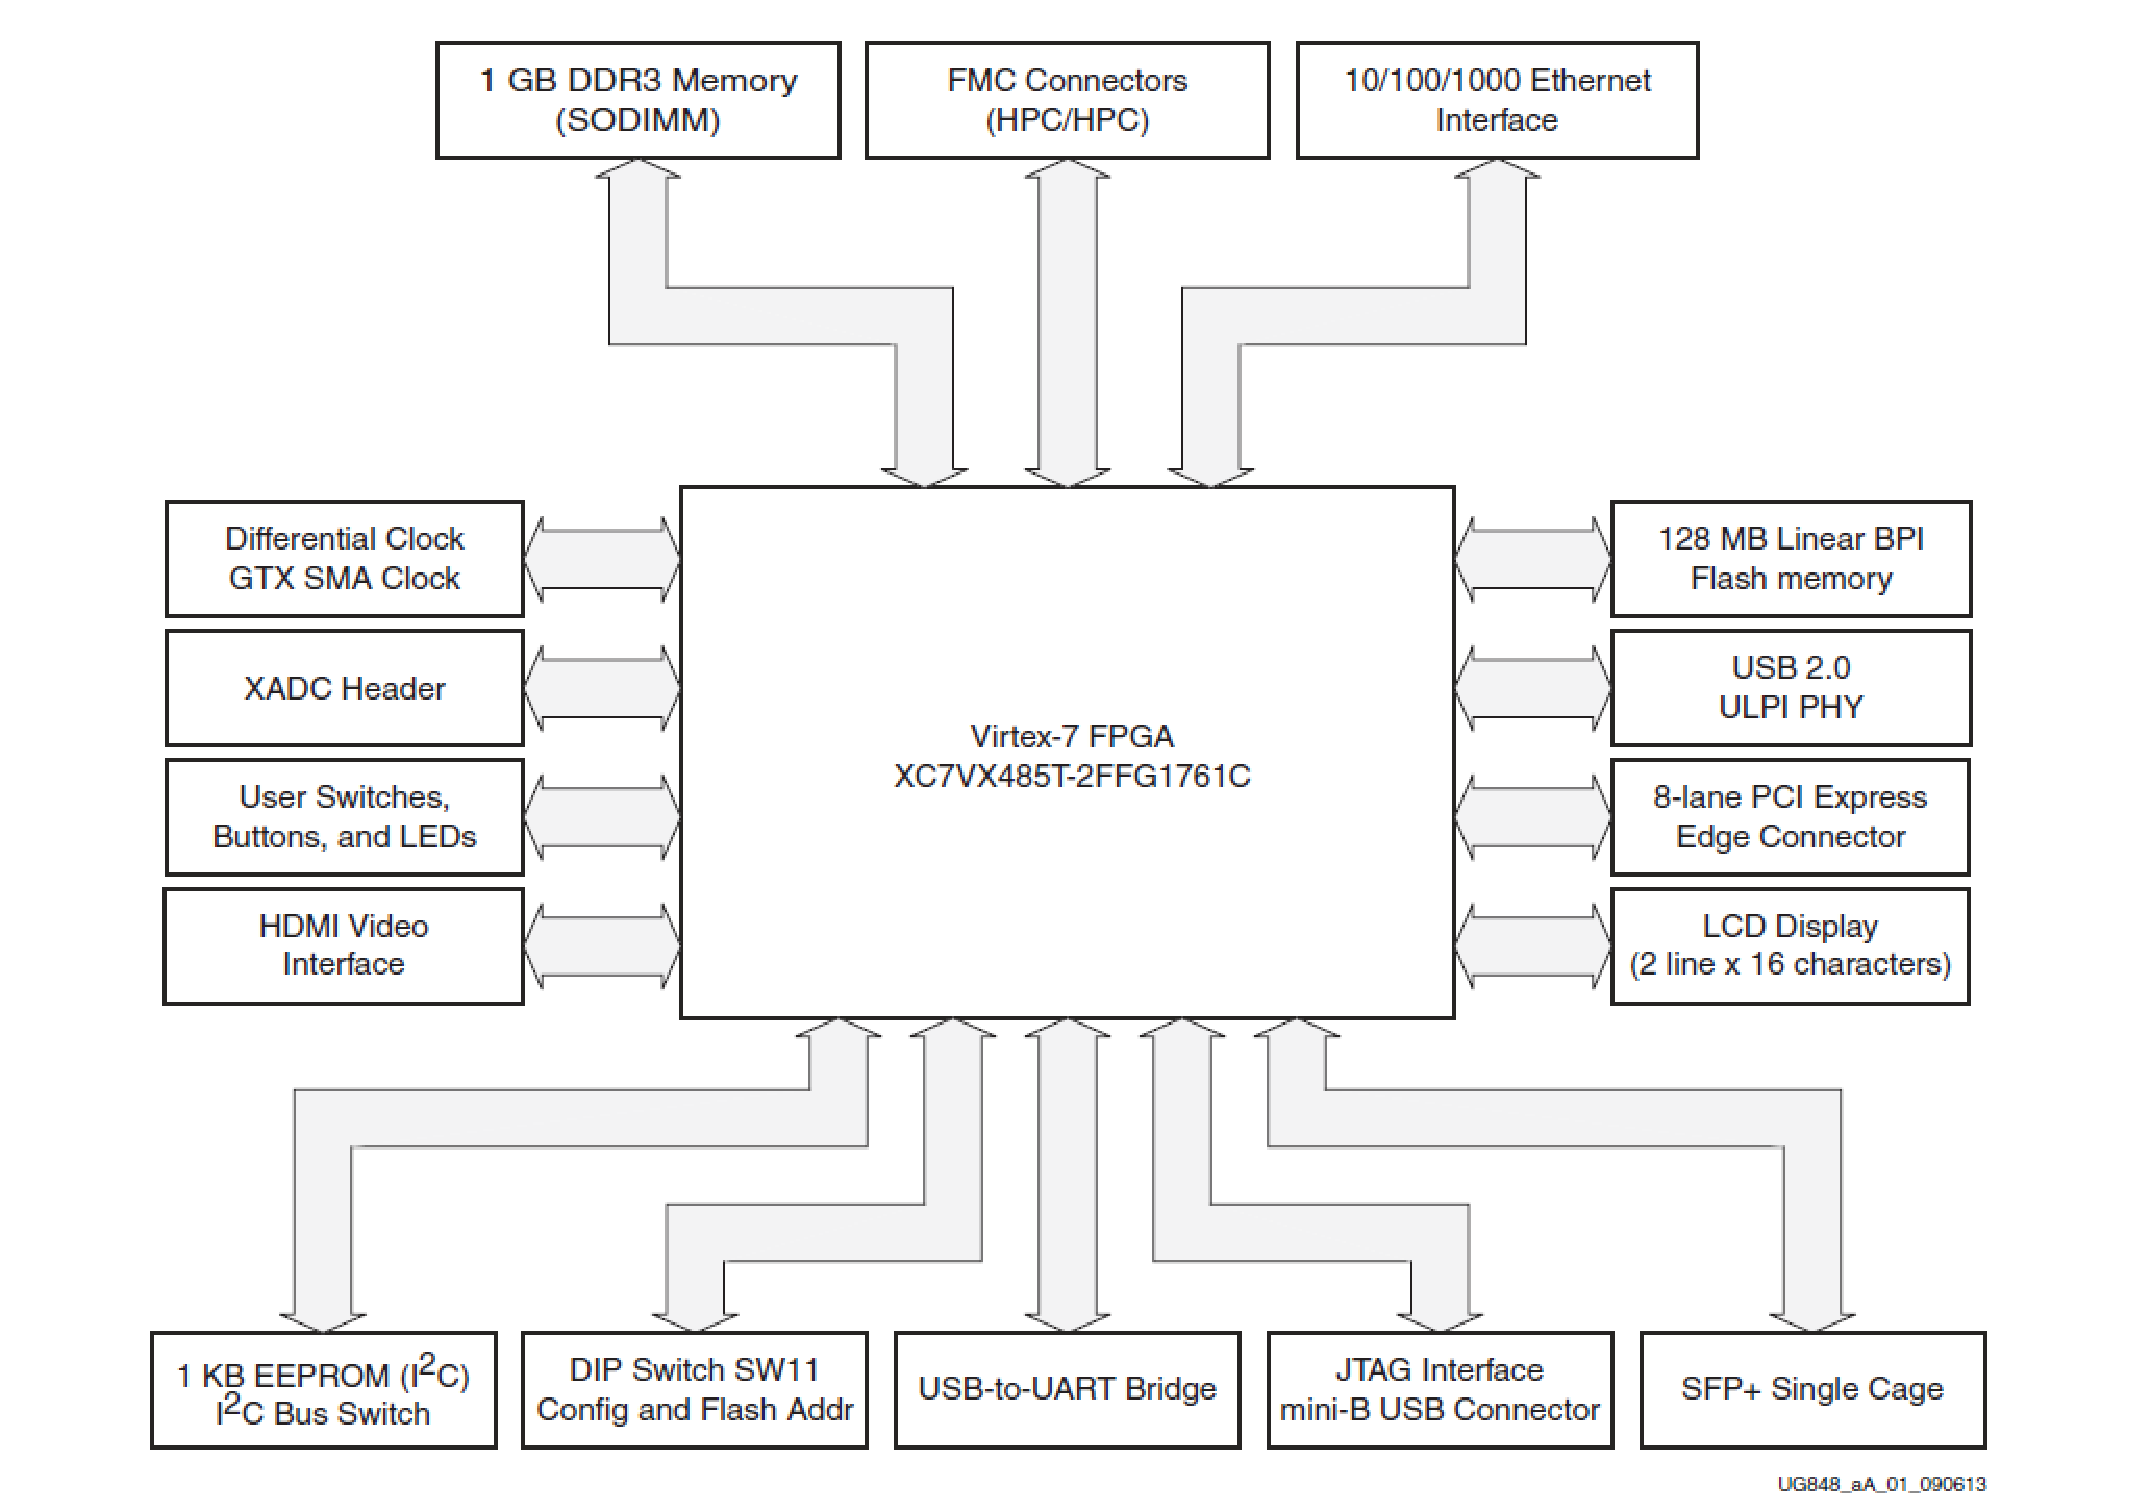
\includegraphics[width=0.65\textwidth]{./figures/vc707_bd}
    \caption{ VC707 Functional Block Diagram
    \label{fig:vc707bd}}
\end{figure}

\subsection{IP Cores}

Xilinx Design Tools have a methodology of developing by using IP blocks, IP
stands for intellectual Property, it means that, it is possible to develop some
functionality or block and sell the right to use it for other developers, fact
which makes development a lot faster and easier.

Xilinx provide IP cores for all the development boards devices and components,
thus this part aims to briefly describe the blocks used in this work. Other
companies that develop peripherals to be integrated with Xilinx FPGAs also have
to develop and provide their own IP cores, like the FMComms2 board which has its
transceiver IP.

%escrever um pouco sobre os ips usados

\begin{description}
	\item[Microblaze \cite{xilinx:ublaxe}] \hfill \\

Microblaze is a soft processor core designed for Xilinx FPGAs, MicroBlaze is
implemented entirely in the general-purpose memory and logic fabric of Xilinx
FPGAs and synthesized inside the FPGA, it has a 32 bit instruction set and runs
usually at 100 Mhz clock, and has only one interrupt input. The Microblaze function
in this system is basically to initialize all the software drivers, configure
such drivers and execute interrupt routines.

Below it is possible to see a block schematic of microblaze core:

%ublaze block diagram
\begin{figure}[htbp]
    \centering
    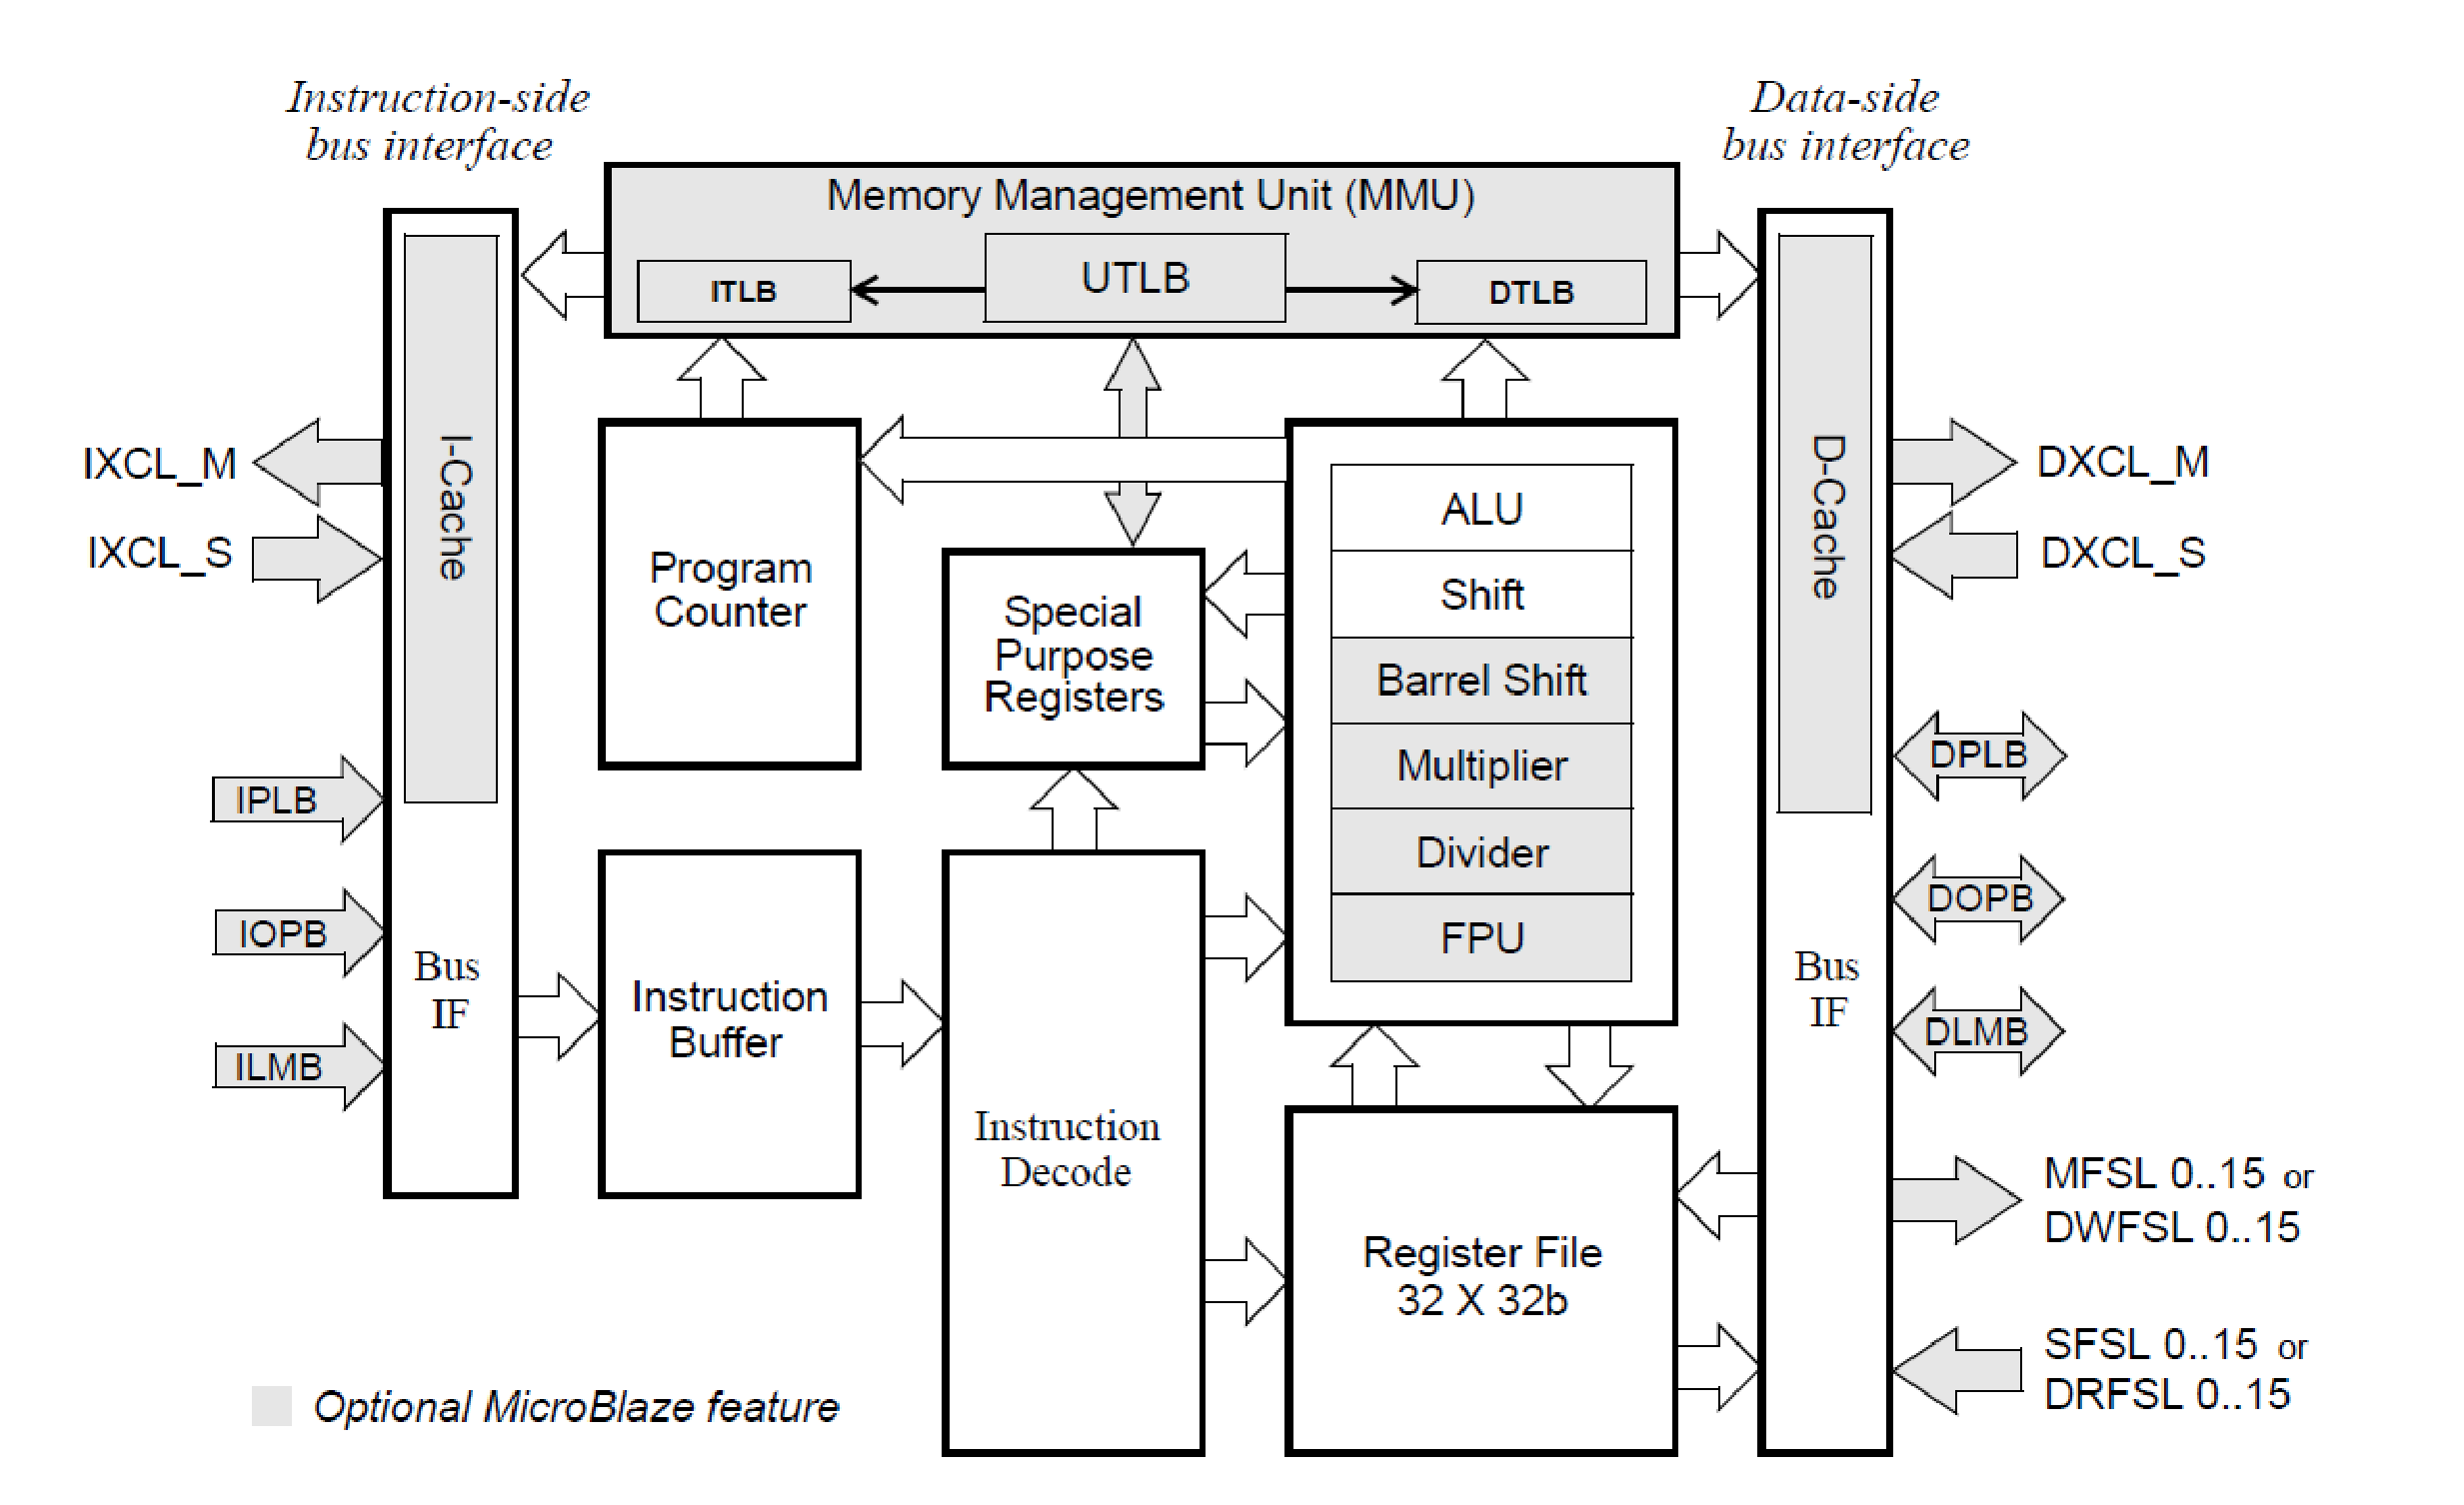
\includegraphics[width=0.65\textwidth]{./figures/mb_bd}
    \caption{ Microblaze core Block Diagram
    \label{fig:mbbd}}
\end{figure}

	\item[DMA Engine \cite{xilinx:axidma}] \hfill \\

  The DMA is the core which makes possible reading and writing from the memory in
a very fast rate. There are various modes of operation, but in this project the
Scatter gather mode is used, in this mode the reading and writing is possible in
a non-continuous memory addresses by the use of block descriptors.

%dma block diagram
\begin{figure}[htbp]
    \centering
    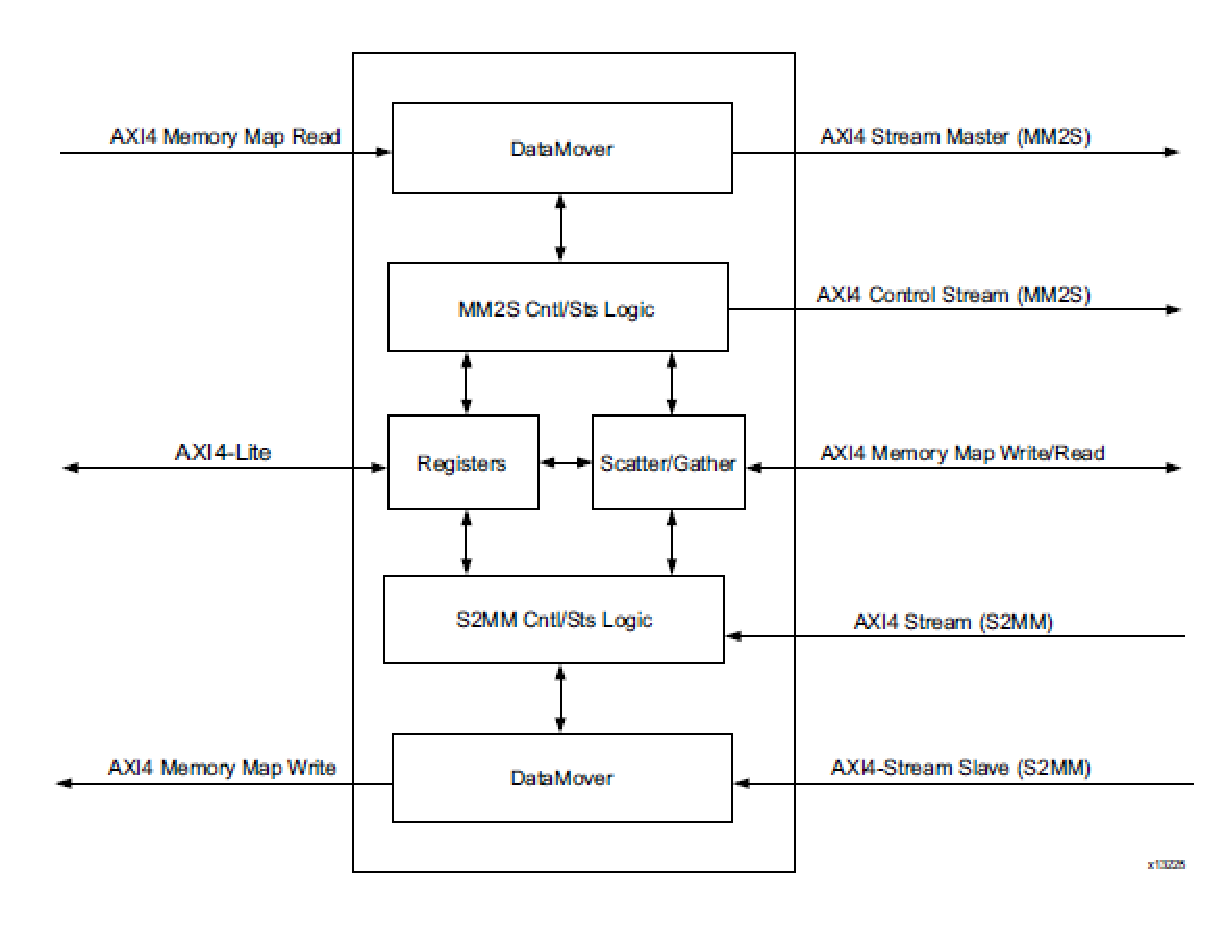
\includegraphics[width=0.65\textwidth]{./figures/dma_bd}
    \caption{ AXI DMA Block Diagram
    \label{fig:dmabd}}
\end{figure}

  \item[Memory Interface Generator \cite{xilinx:mig7}] \hfill \\

  The MIG (Memory interface generator) creates a software and hardware interface
to the DDR3 memory inside the FPGA board.

  \item[SPI \cite{xilinx:axiquadspi}] \hfill \\

  The SPI is a communication protocol, thus the SPI core  is used to write/read
registers in the FMComms2 board. It is hardware initializable and controllable.

  \item[GPIO \cite{xilinx:axigpio}] \hfill \\

  GPIO stands for General Purpose Input and Output, this core implements general
purpose pins which can be configured via software to act as an input or output pin,
or even both. For this project specifically, GPIO core is used to make real-time
operations in the AD9361 internal state-machine and for reset.

  \item[UART \cite{xilinx:axiuart}] \hfill \\
  UART is also a communication protocol and stands for universal asynchronous
receiver/transmitter and in this case it is used for debugging purposes, all the
standard I/O form the software comes from the UART and it is possible to show
error messages and status messages from the code in the terminal, like any normal
print, but such messages are comming from the FPGA elf file being executed in the
Microblaze soft processor.

\end{description}


%--------------------------------FMCOMMS2---------------------------------------
\section{Transceiver - FMComms2}
\subsection{AD9361}
\label{subsec:ad9361}

The AD9361 is a high performance RF transceiver. Its programmability and
adaptability makes it ideal for a wide range of transceiver applications. This
device combines a RF front end with a flexible and configurable mixed-signal
baseband section and frequency synthesizers, simplified configuration digital
interface to a processor. The AD9361 operates from 70 MHz to 6.0GHz range with
supported channel bandwidths from 200 KHz to 56 MHz and the AD9361 is a 2 Rx and
2 Tx device packed in a 10mm x10mm, 144 ball chip package ball grid array
(CSP\_BGA).

\subsubsection{General Description}

AD9361 is a highly integrated RF frequency transceiver capable of being
configured for a wide range of applications, including 3G and 4G frequency
applications. AD9361 and AD9364 almost the same hardware and specifications, the
difference is that AD9361 is a 2x2 MIMO and AD9364 is a 1x1
\cite{web:ad9361wiki}. The programmability allows the AD9361 to be operated in
Frequency Division Duplex (FDD) and Time Division Duplex (TDD) systems, allowing
this transceiver to operate in a variety of communication standards. Another
interesting feature is the capability of integration with a wide range of BBPs
(Baseband Processors) using a single or dual 12-bit parallel data port or a
12-bit LVDS (Low voltage Differential signaling), which uses the FMC connector
in the FMCommS2. AD9361 also provides self-calibration and automatic gain
control (AGC) systems to maintain good performance under variable conditions,
such as temperature and signal quality. The transceiver has also various modes
of test mode with the Built-in Self Test (BIST) modes which can be used for the
designers to debug designs during prototyping. This configurability and
adaptability is very attractive for Software Defined Radio (SDR) and for C-RAN
systems, indeed AD9361 is already being used in some Universal Software Radio
Peripheral (USRP) from Ettus research (National Instruments) \ref{sd:usrp}, this
alone is a proof that AD9361 can work in a wide range of systems and standards,
below there is a functional block diagram od the AD9361 chip
\ref{fig:ad9361func}.

\begin{figure}[htbp]
    \centering
    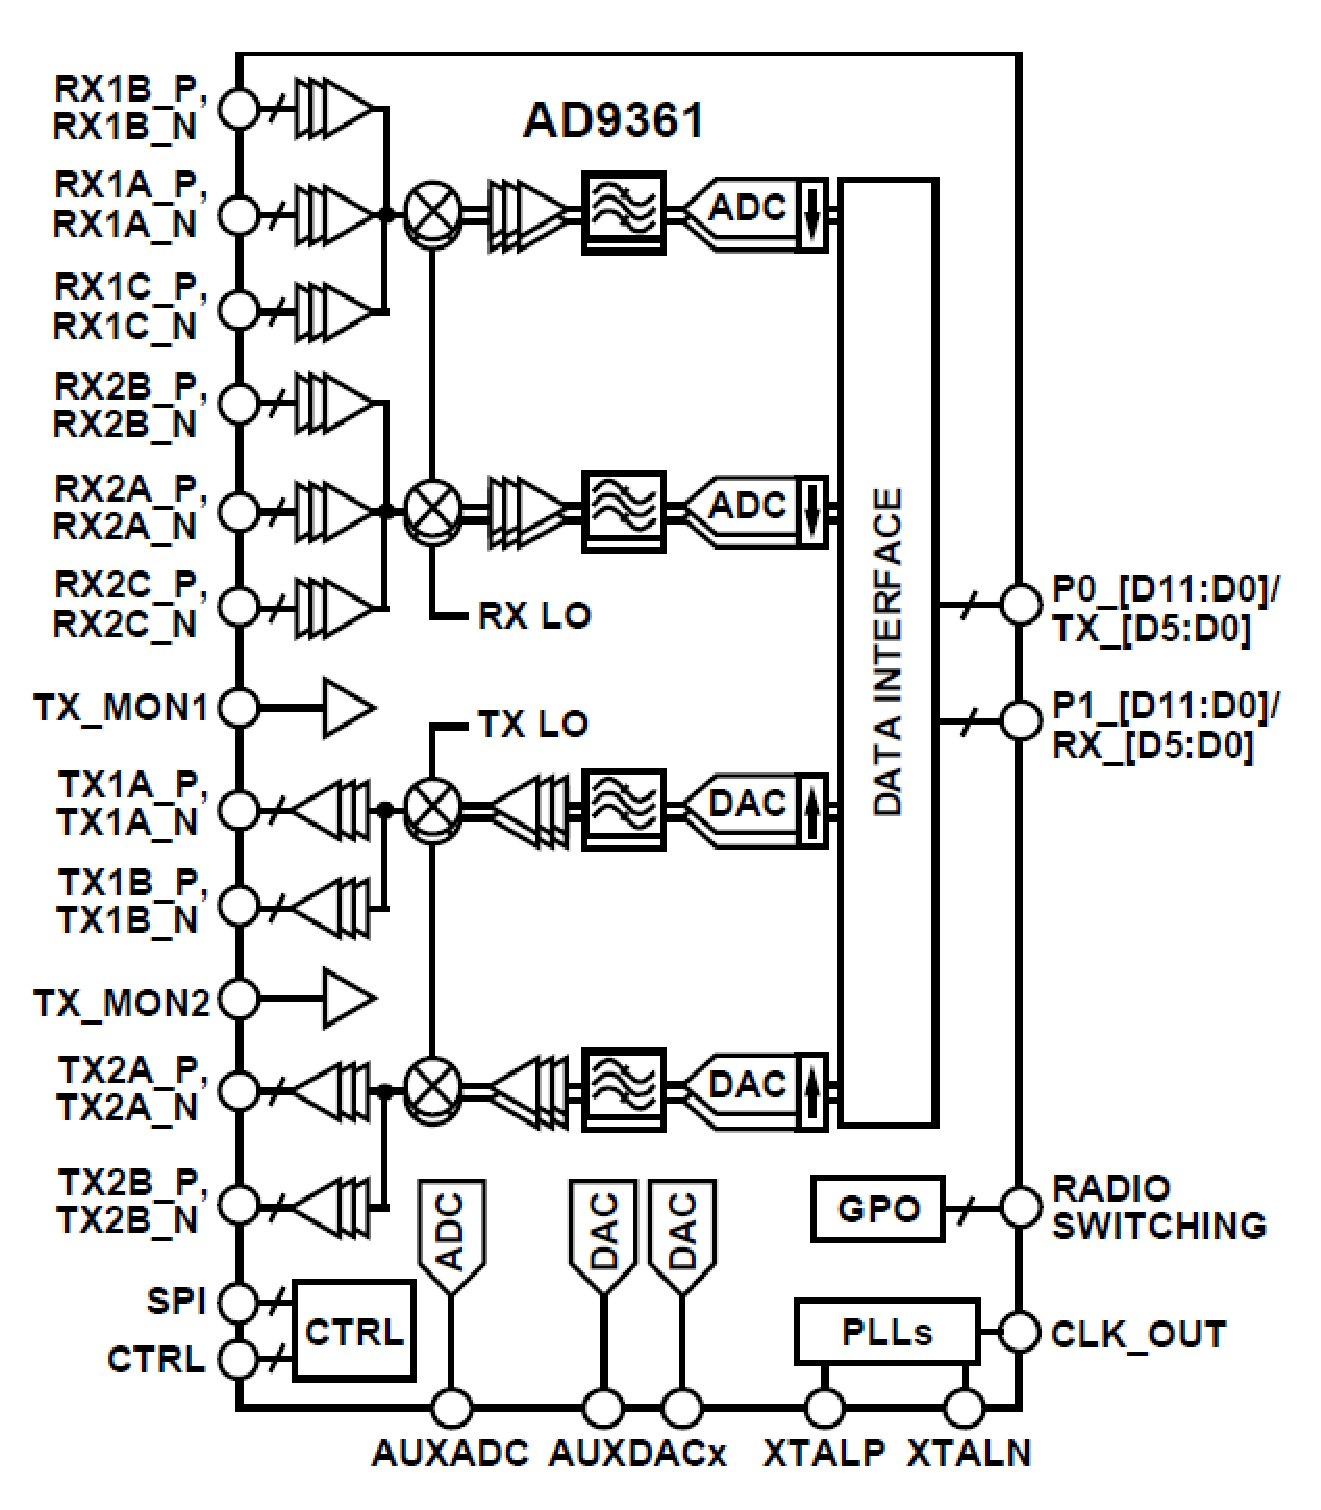
\includegraphics[width=0.45\textwidth]{./figures/ad9361_functional_diagram}
    \caption{ AD9361 Functional Block Diagram
    \label{fig:ad9361func}}
\end{figure}

\subsubsection{Receiver}

The receiver section has all the blocks necessary to receive analog RF signals
and convert them to digital data which can be used by the BBP. there are two
independently controlled channels that share same frequency synthesizer. This
characteristic makes possible to the AD9361 to operate in MIMO systems.

Each channel has 3 inputs which can be multiplexed into the signal chain, making
possible to use the AD9361 into systems with multiple antenna inputs. The
Receiver is a direct conversion system that contains a Low noise amplifier (LNA) ,
followed by a matched in-phase and quadrature amplifier, mixers, and band
shaping filters that down convert received signals to baseband for digitization.
External LNAs can also be interfaced to the AD9361 allowing more flexibility in
the design. The receiver signal path passes down-converted signals (I and Q),
which are schematically identical to each other,  to the baseband (BB) receiver
section. The BB section is composed by two programmable low-pass filters, with
programmable corner frequency for each filter, 12-bit ADC and four stages of
decimating filters, each of the four decimation filters can be bypassed. The
gain control is achieved by a preprogrammed gain index map, a lookup table for
example, this map distributes gain in order to achieve optimal performance at
each level. This optimal behavior can be achieved by enabling AGC, which can run
in two modes, fast and slow gain control. This allow for the BBP to make gain
adjustments as needed. Each channel also contains independent RSSI measurement
capability, DC offset tracking and all other circuitry needed for
self-calibration.

The receiver ADC is a 12-bit sigma-delta ($\Sigma-\Delta$) ADC which allows
adjustable sample rates. This ADC produces data streams from the received
signals and such digitalized signals can be conditioned further by a series of
decimation filters and a 128-tap FIR filter with additional decimation settings.
The sampling rate of each digital filter is adjustable through changes in the
decimation factors to produce the needed data rate.\\

In short, the Receiver chain , in figure \ref{fig:rxchain}, has:

\begin{itemize}
	\item LNA - Low noise Amplifier
	\item Matched in-phase amplifier;
	\item Quadrature Amplifier;
	\item Band Shaping Filters;
	\item Analog low pass filters;
	\item 12-bit DAC;
	\item 4 stages of decimation filters (128-tap FIR filters);
	\item Automatic gain Control;
\end{itemize}

\begin{figure}[htbp]
    \centering
    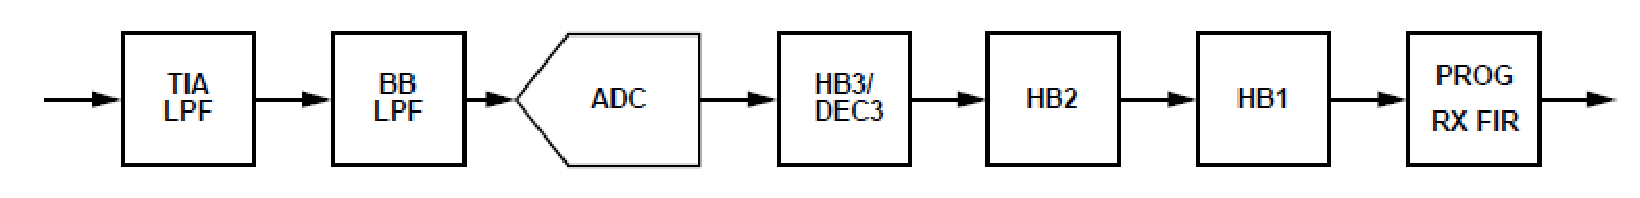
\includegraphics[width=0.65\textwidth]{./figures/rx_chain}
    \caption{ Receiver Signal Path
    \label{fig:rxchain}}
\end{figure}


\subsubsection{Transmitter}

Like the receiver section, the transmitter section contains two identical and
independently controller channels, which share the same frequency synthesizer,
that provide all digital signal processing, mixed signal and RF blocks necessary
to implement a direct conversion system from digital data to RF. The Tx signal
path receives from the BBP 12-bit 2s complement I-Q format data in the digital
interface and each channel goes through a 128-tap FIR filter with interpolation
options, which is fully programmable. Then the signal goes through a series of
additional interpolation filters that manipulates the signal with additional
filtering and data rate interpolation before reaching the 12-bit DAC, note that
all these filtering and interpolation steps can be bypassed if desired. Each
12-bit DAC has an adjustable sampling rate and its analog output passes through
to low pass filters to remove any sampling artifacts before going to the RF
mixer, these low pass filters corner frequencies can be programmable too. After
all these filtering and analog conversion steps, the I and Q signals are
recombined and modulated in the carrier frequency, which can be adjusted by
changing the synthesizer frequency. These analog combined signals passes through
additional analog filters for better band shaping and then it can be transmitted
to the output amplifier. Each Transmitting channel provides wide attenuation
adjustment range with fine granularity in order to optimize SNR.

\begin{figure}[htbp]
    \centering
    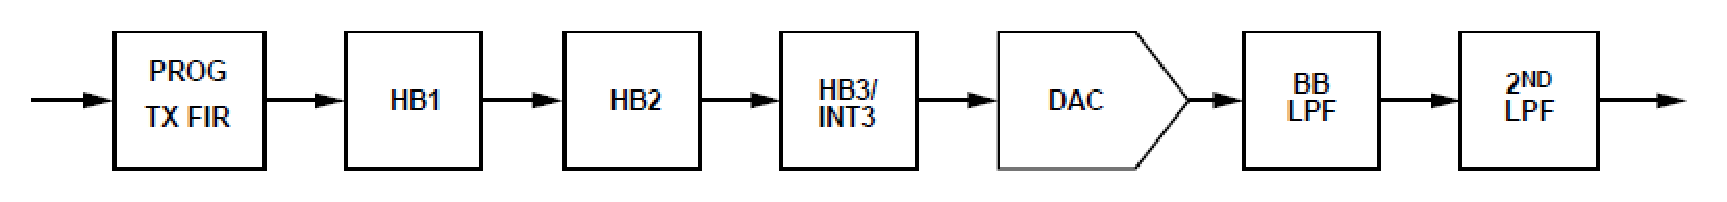
\includegraphics[width=0.65\textwidth]{./figures/tx_chain}
    \caption{ Transmitter Signal Path
    \label{fig:txchain}}
\end{figure}


Identical to the receiver chain, the transmitter chain , in figure
\ref{fig:txchain} has also built-in self-calibration circuitry into each
transmitting channel providing an automatic real-time adjustment. The
transmitter also provides a TX monitor block for each channel, this block
monitors the transmission output and routes it back through an unused receiver
channel to the BBP for signal monitoring, but these monitoring option is only
available in TDD mode operation while the receiver is idle.

In short the transmission chain has:

\begin{itemize}
	\item 128-tap FIR filters;
	\item Interpolation Filters;
	\item 12-bit DAC;
	\item Analog Low-pass Filters;
	\item Additional band shaping analog filters;
	\item Attenuation adjustment;
	\item self-calibration circuits;
	\item Tx signal Monitor.
\end{itemize}

In the figure \ref{fig:ad9361blk} below there is a full block diagram with both
\textit{receiver Chain}, \textit{Transmitting Chain} and other key components of
the AD9361 chip.

\begin{figure}[htbp]
    \centering
    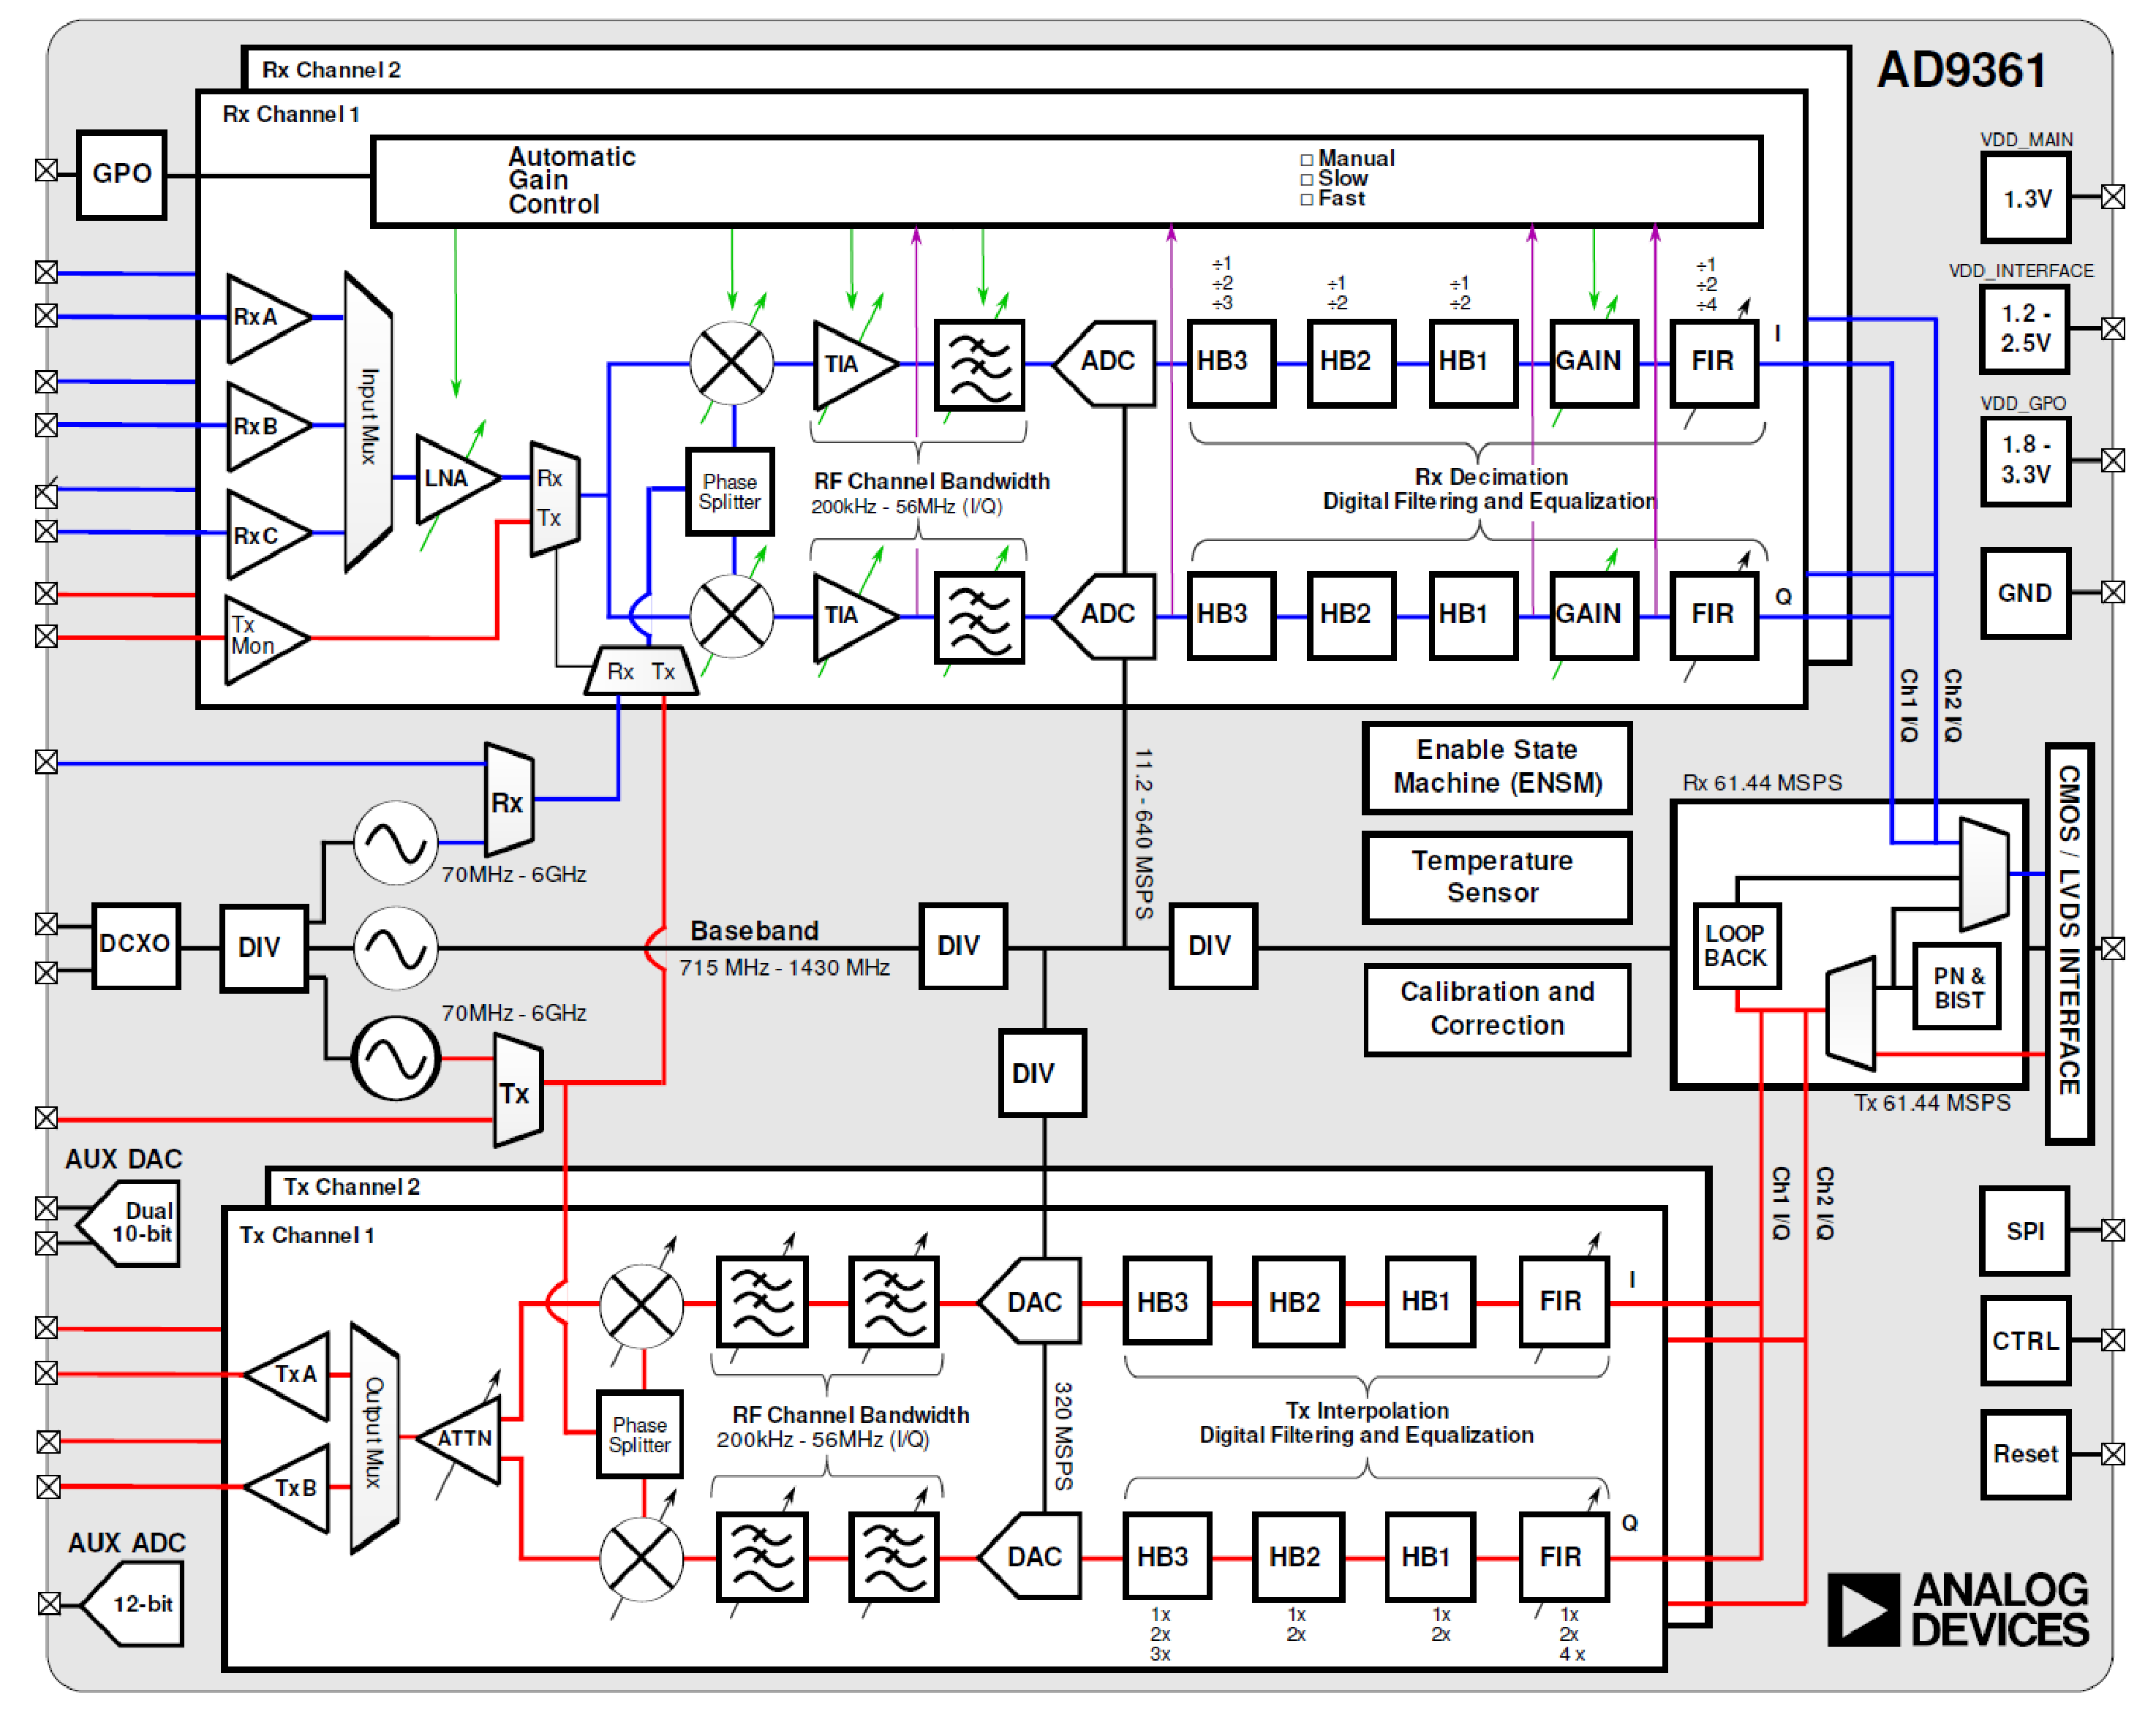
\includegraphics[width=0.65\textwidth]{./figures/ad9361_block_diagram}
    \caption{ AD9361 Block Diagram
    \label{fig:ad9361blk}}
\end{figure}

\subsubsection{Filtering}

In both receiver and transmitter there are:
\begin{description}
	\item[Receiver] \hfill \\
	\begin{itemize}
		\item Low pass filter : band shape to reduce adjacent-channel interference.
		\item Decimation Filter: up convert from the digital baseband rate (64.11MSPS max) to the actual ADC (640MSPS) rate.
	\end{itemize}
	\item[Transmitter] \hfill \\
\begin{itemize}
		\item Low pass filter : remove sampling artifacts
		\item Interpolation Filter : down convert from the digital baseband rate (64.11MSPS max) to the actual DAC (320MSPS) rate.
	\end{itemize}
\end{description}

In both digital and analog implementations these filters have impact the
magnitude and the phase in passband, such behavior must be compensated in the
system, and this compensation is usually done inside the 128-tap FIR filter. The
FIR filter is not only used for low pass filter realization but also to
compensate for magnitude and phase impacts created by the analog and digital
half band filters in the desired baseband area.

These filters depend in various other systems to work properly, such systems are
sample rates, clock, data rates which sets the half band filters, and the
desired RF bandwidth, which sets the analog filters. the process of loading a
filter and after changing anything in the system will negatively affect the
overall baseband performance.

There is a filter too created by analog devices,which designs a low-pass filter
and sets the FIR coefficients in order to ensure compensation for magnitude and
phase changes in the analog or half band filters.
\subsubsection{Clocking}

%reescrever
The AD9361 has a series of internal PLL to generate and manipulate clock
signals. There are fractional-n PLLs that generate the transmitter and receiver
LO frequencies and there are the baseband PLL (BBPLL) used for the data
converters, digital filters and I/O ports. All the frequency signals are
generated using these PLLs clock outputs.

All the PLLs require a reference clock input and for this there is the digitally
controlled oscillator (DCXO) function, which is an in-chip programmable and
variable capacitor, such capacitor can tune the crystal frequency variance
before entering the system, having a precision of +/- 6 ppm it results in a more
accurate reference clock and can be used, if needed, for synchronization
purposes. this function can also be used together with the on-chip temperature
sensor to provide temperature compensation depending enviroment in which the
chip will be used. For the reference clock there are two options:

\begin{description}
	\item[External Oscillator] \hfill \\
	In this option and external clock signal can be connected in the XTALP pin
(Leaving the XTALP pin unconnected), this external clock frequency may vary from
10 MHz to 80 MHz. Such type of setup is needed when a wireless base-station (BTS)
reference clock is locked to a master clock, and in such systems there is no or
less need for clock synchronization.

	\item[Dedicated Crystal] \hfill \\
	In this option a dedicated crystal, with frequency varying from 19 MHz to 50
MHz, is connected in the XTALP and XTALN pins. This setup is usually used in
wireless user equipment (UE), which do not need to be locked to a master clock
but they do need to adjust periodically the LO frequency in order to maintain a
connection with a BTS. The BTS periodically informs the UE of its frequency
error relative to the BTS and the BBP can make adjustments to the reference
clock and thus adjust the LO frequency if needed.

\end{description}

\begin{figure}[htbp]
    \centering
    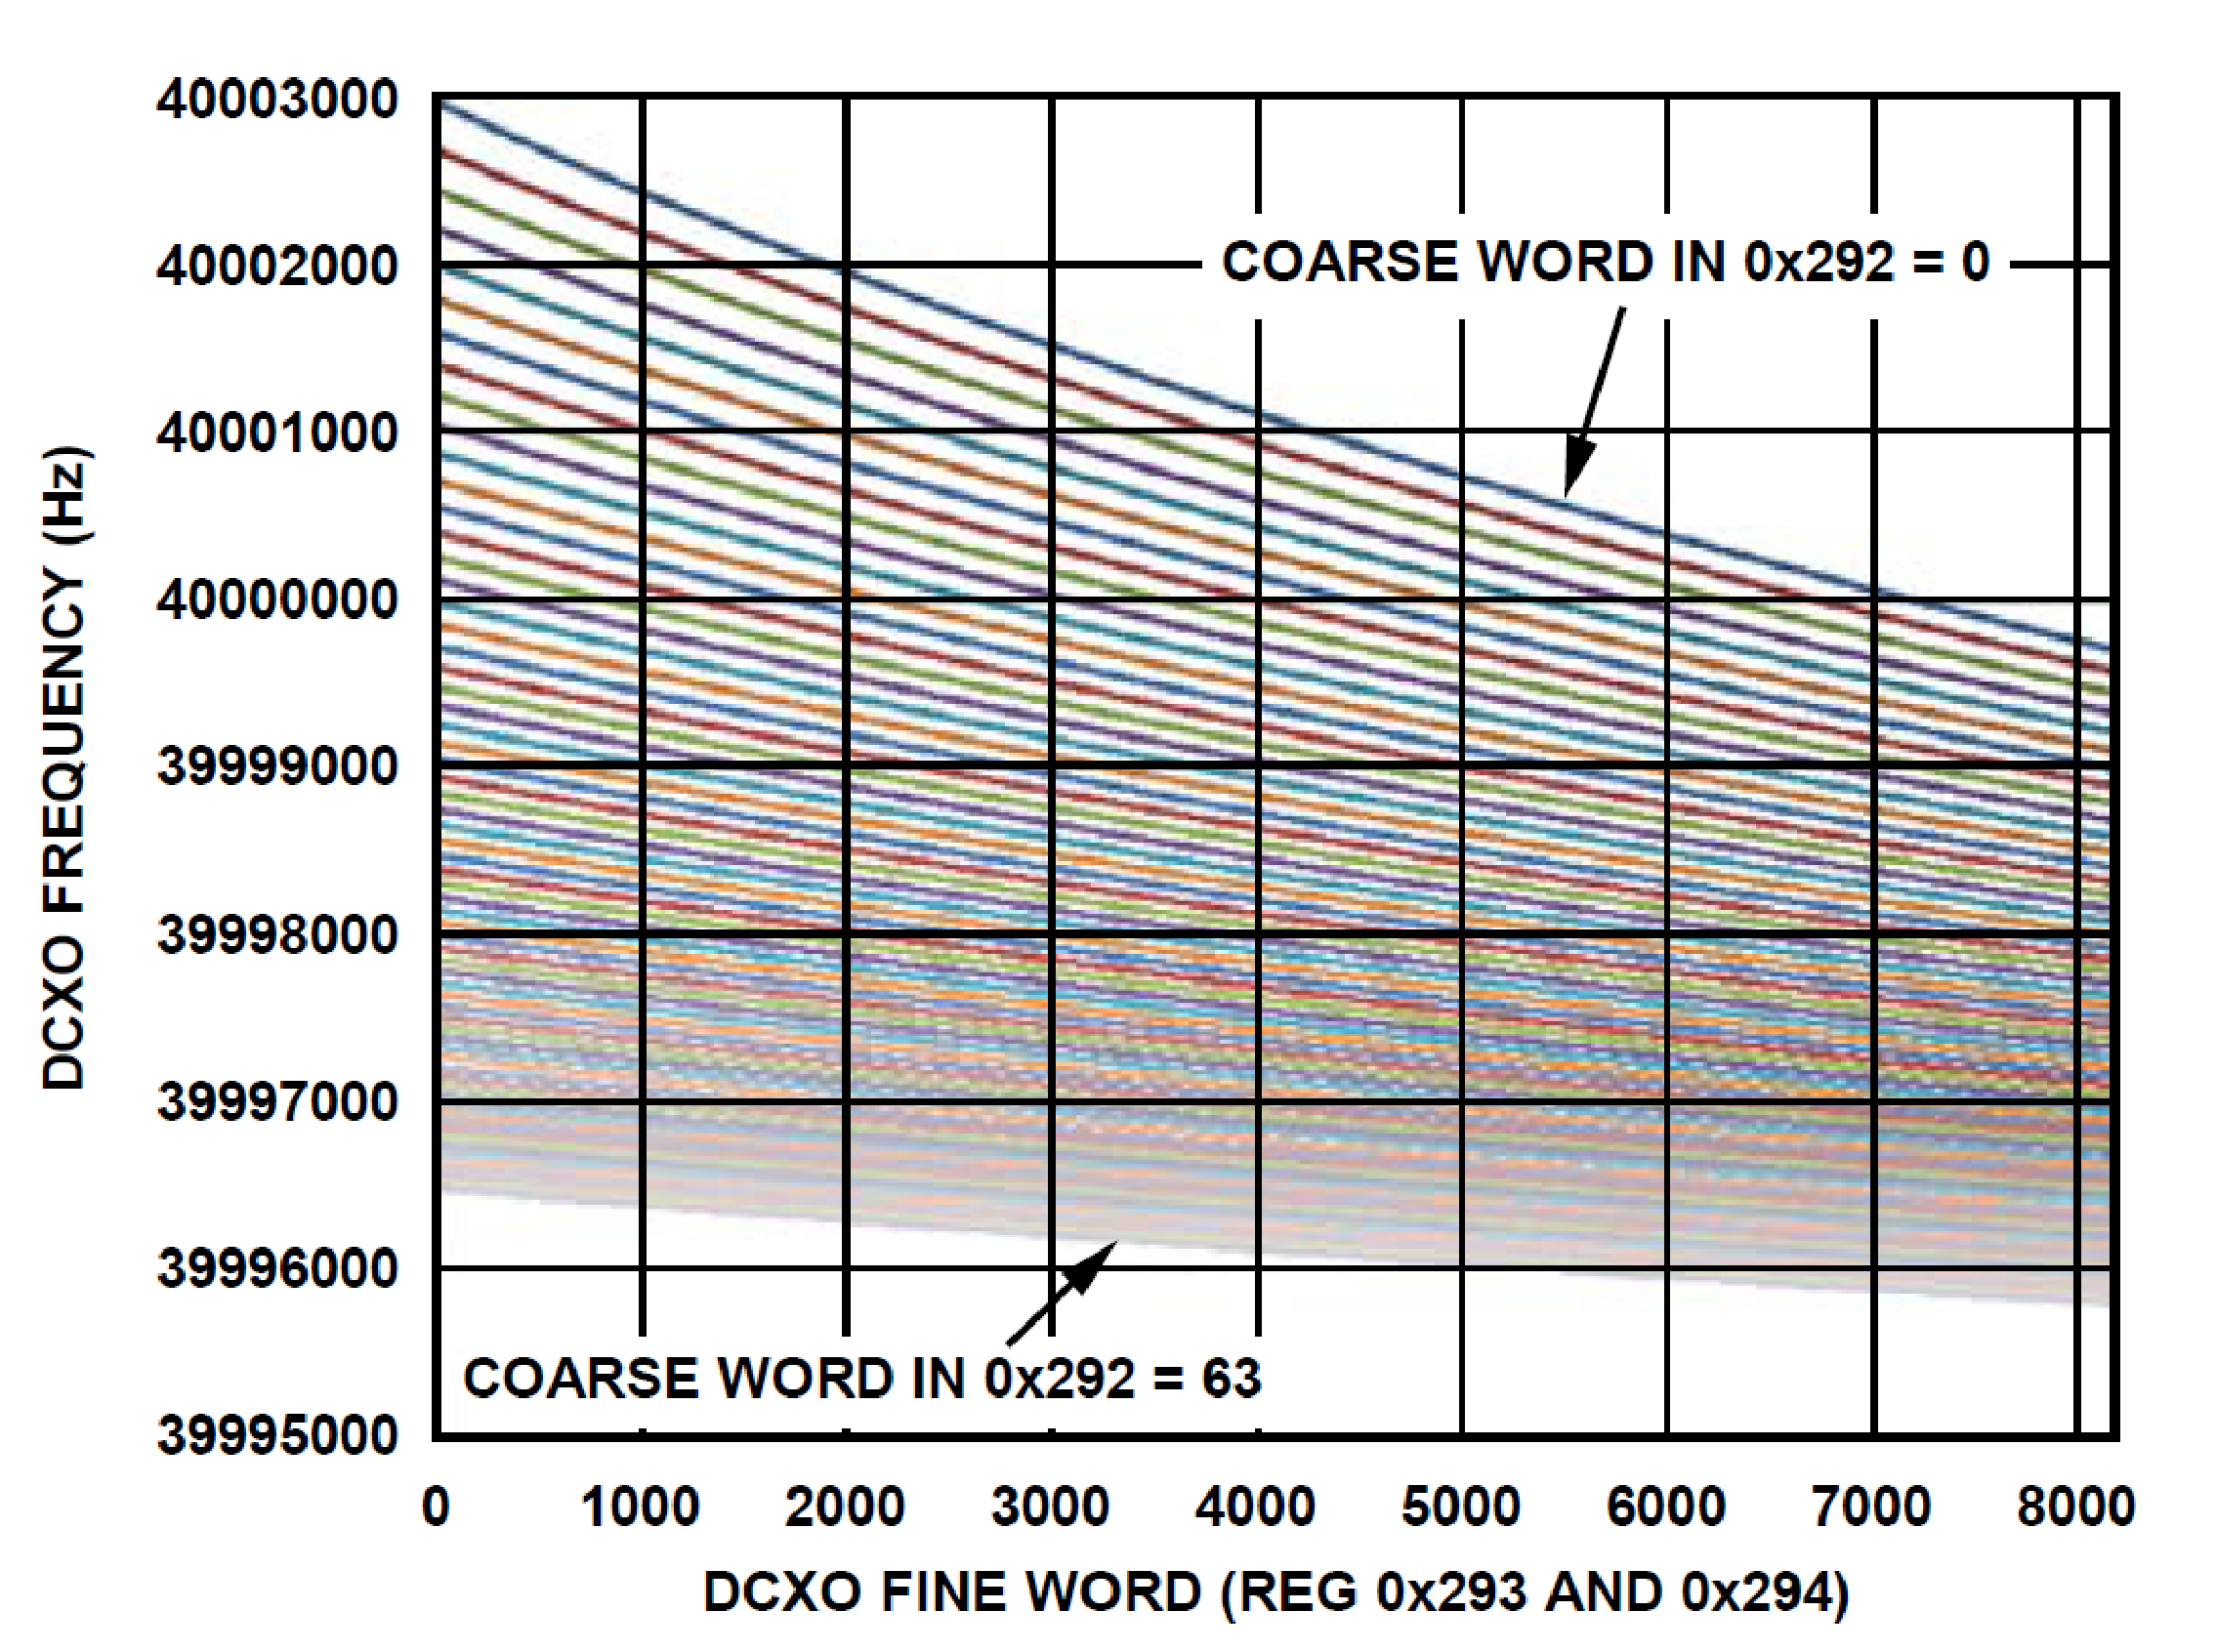
\includegraphics[width=0.45\textwidth]{./figures/dcxo_graph}
    \caption{ DCXO Behavior Graph
    \label{fig:pll}}
\end{figure}

\subsubsection{Synthesizers}

\begin{description}
	\item[RF PLLs] \hfill \\
	The AD9361 contains two identical synthesizers to generate the required LO
signals for the RF signal path, one for the receiver and one for the
transmitter. The PLL synthesizers are fractional-n PLLs with completely
integrated VCOs and loop filters, requiring no other external components. In TDD
operation mode, the synthesizers turn ON and OFF appropriate for the TX and RX
frames, however in FDD TX PLL and RX PLL are activated at the same time.

	\item[BB PLL] \hfill \\
  The AD9361 contains also a baseband PLL synthesizer,
	which generate all the baseband related clock signals. The BBPLL feeds all the
	baseband related clock signals to ADC, DAC (Sampling Clock), DATA\_CLK signal
	and all data framing signals. This PLL has a frequency range from 700 Mhz to
	1400 Mhz, and can be changed based on system requirements.

\end{description}

\begin{figure}[htbp]
    \centering
    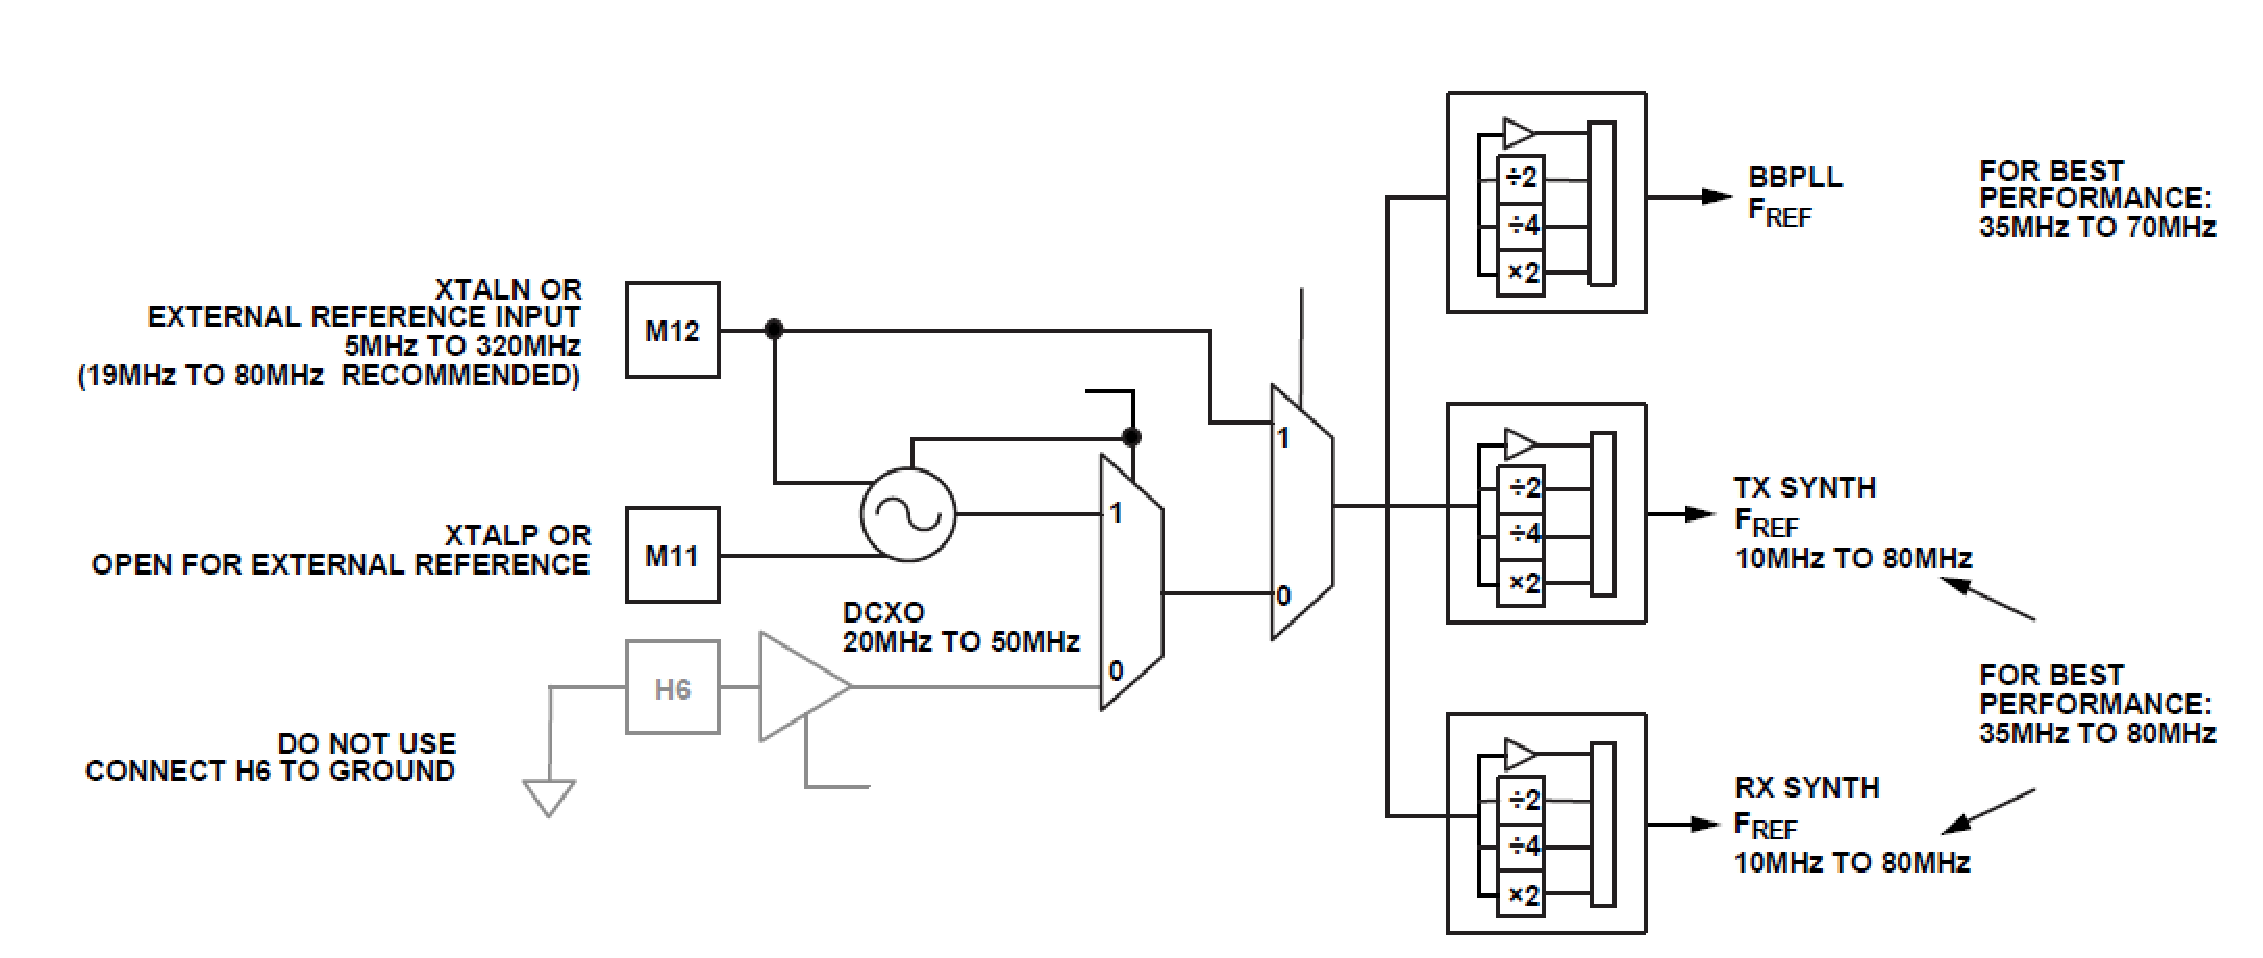
\includegraphics[width=0.65\textwidth]{./figures/pll_ref_block}
    \caption{ AD9361 PLL Reference Block Diagram
    \label{fig:pll}}
\end{figure}

\subsubsection{Digital Data Interface}

The AD9361 uses parallel data ports to transfer data between the device and the
BBP. These data ports can be configured either single-ended CMOS format or LVDS
format (used in this work). Both formats can be configured in multiple
arrangements to adequate the system requirements for data transfer and
connections. These arrangements can be of single port data bus, dual port data
bus, single data rate, double data rate and other various combinations
compatible with the device.

Bus transfers are controlled using hardware handshake signalling, these two
ports can be operated in TDD (bidirectional) or FDD (full duplex) where half of
the bits are used for transmitting and the other half is used for receiving. The
interface can also be configured to use only one of the data ports ( usually
used in applications that do not require high data rates or samples).

The communication between the BBP processor and the AD9361
rely on some signals to properly work, which are DATA\_CLK, FB\_CLK and
RX\_FRAME, its operation is detailed below:

\begin{description}
	\item[DATA\_CLK Signal] \hfill \\
	 RX sends the signal DATA\_CLK to the BBP, which can be used when receiving data.
   DATA\_CLK can be used to control data sampling time, which can be single data
   rate (data is captured on rising clock edge) or double data rate (data is
   captured on both rising and falling clock edges). This can be applied using
   single or dual data port.

	\item[FB\_CLK Signal] \hfill \\
	The FB\_CLK signal must have the same frequency and duty cycle as DATA\_CLK and
like DATA\_CLK it is used as timing reference for the interface. FB\_CLK allows
source synchronous with rising edge capture for burst control signals and can be
used like DATA\_CLK for rising edge, single data rate mode or in both edge
capture, double data rate mode for transmit signal bursts.

	\item[RF\_FRAME Signal] \hfill \\
	The RF\_FRAME signal is generated by the device whenever the receiver outputs
valid data. RF\_FRAME has two modes:
	\begin{itemize}
		\item \textbf{Level Mode:} RF\_FRAME stays high as long as the data is valid.
		\item \textbf{Pulse Mode:} RF\_FRAME pulses with 30\% duty cycle.
	\end{itemize}
	The BBP must provide a TX\_FRAME that indicates beginning of a valid data
transmission with a rising edge. The TX\_FRAME operates similarly as the
RF\_FRAME, on Level Mode or Pulse Mode.

\end{description}

\begin{figure}[htbp]
    \centering
    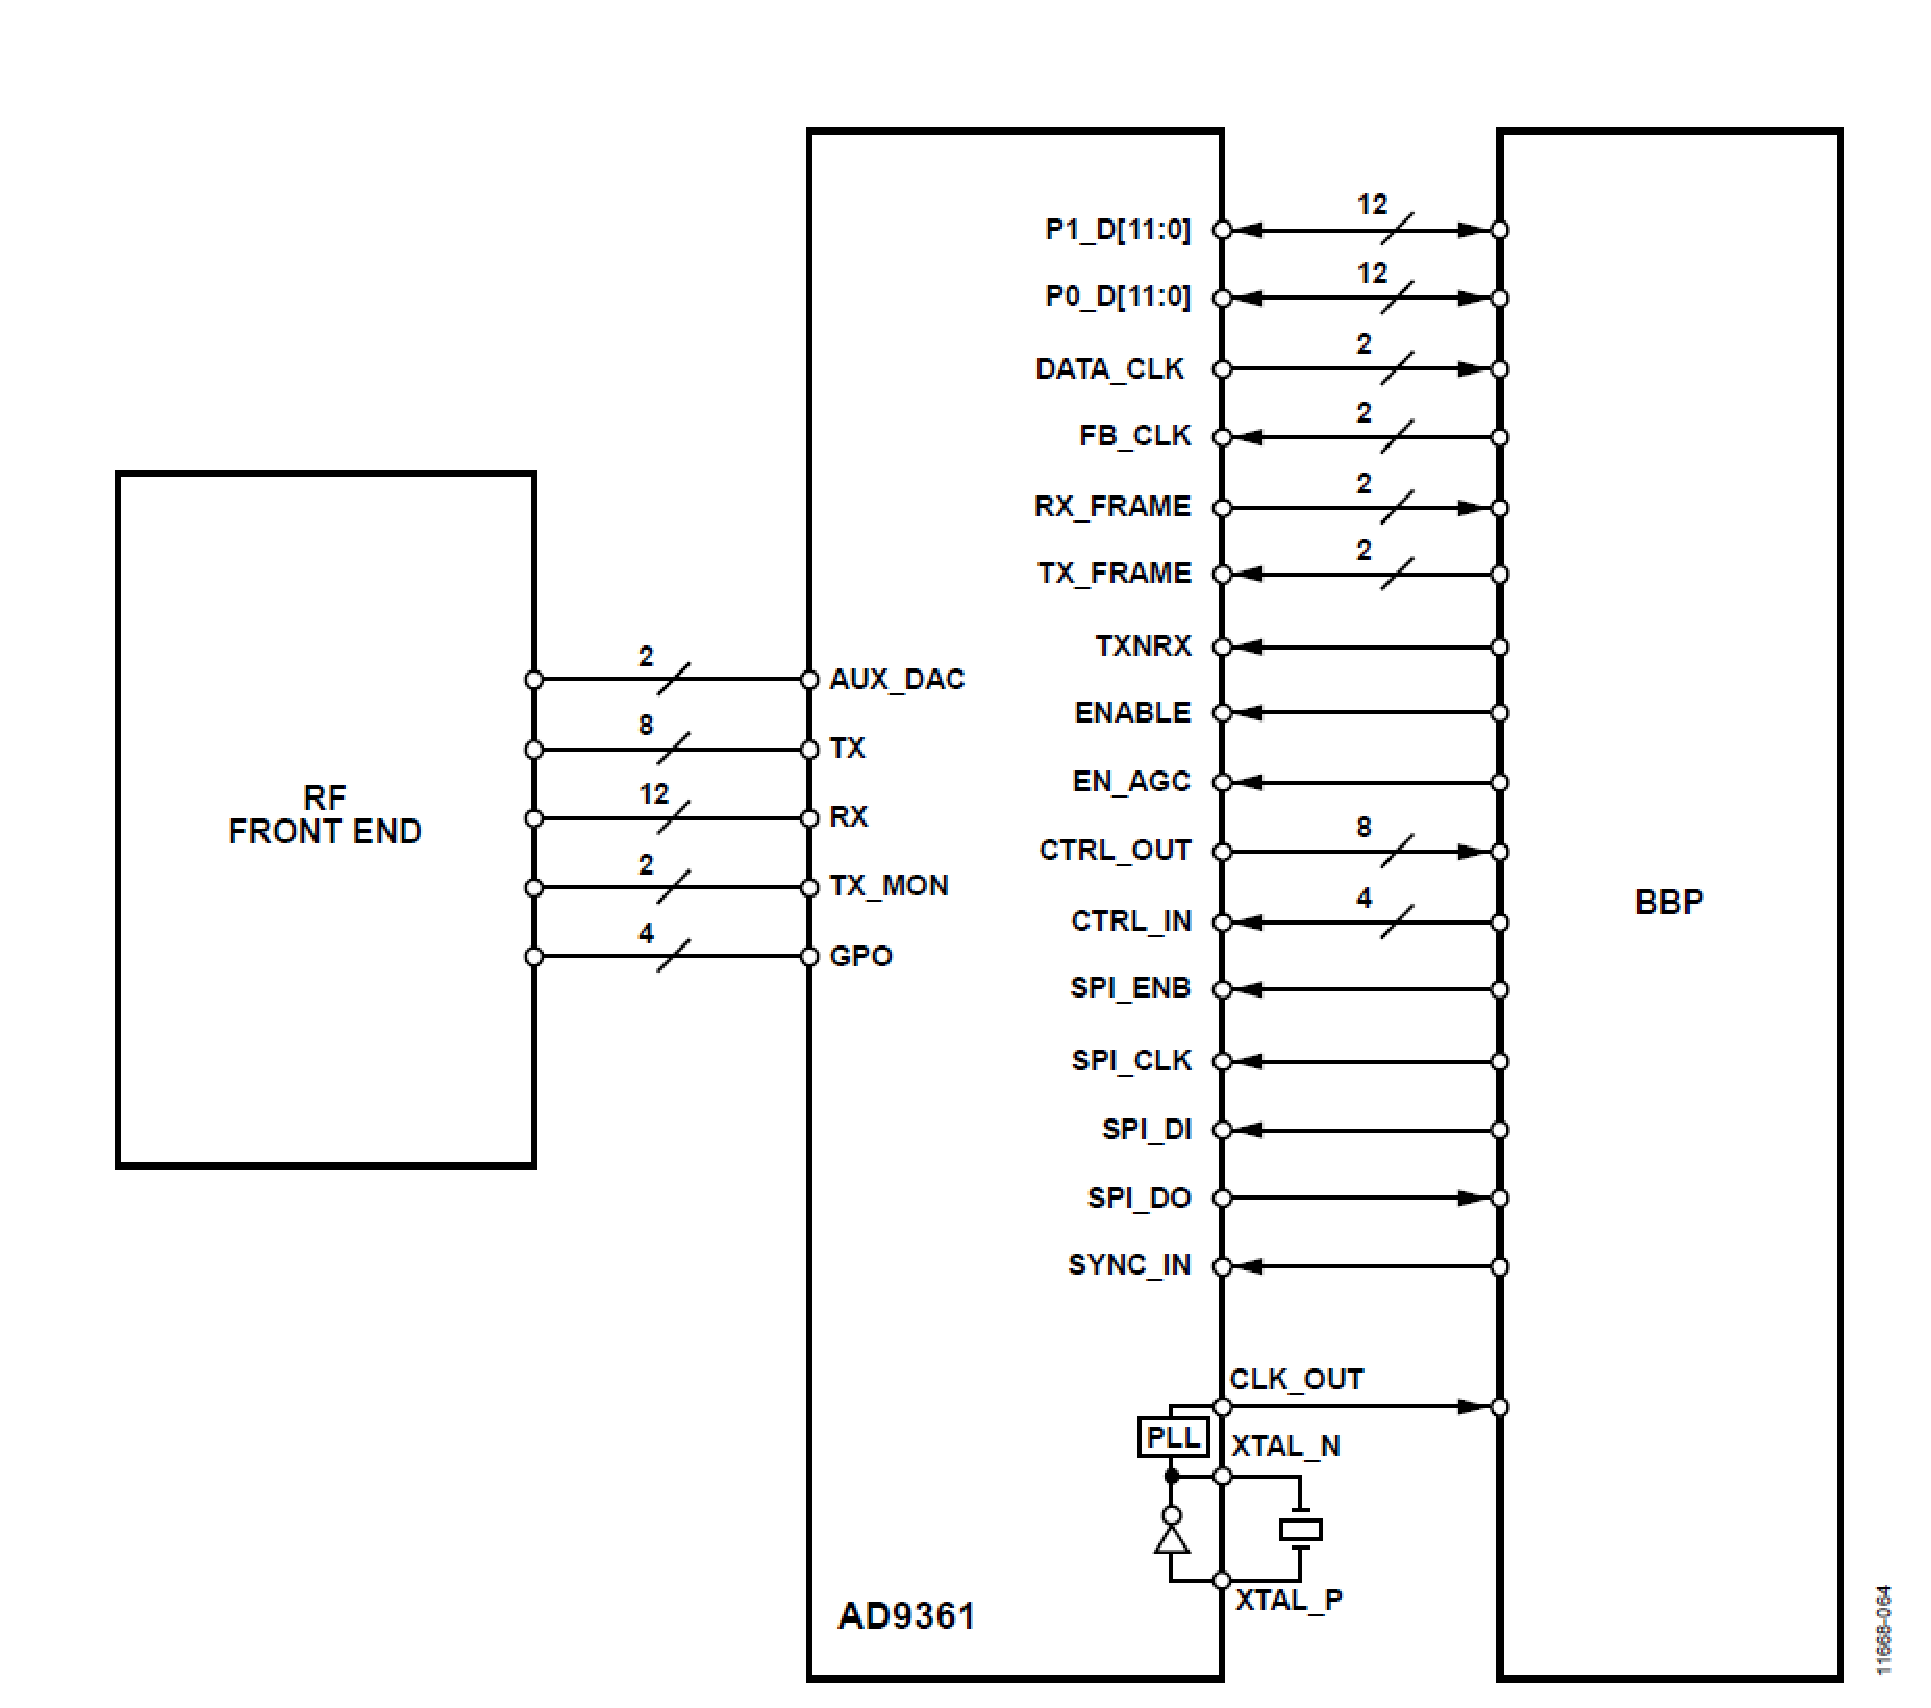
\includegraphics[width=0.45\textwidth]{./figures/ad9361_digital_interface}
    \caption{ AD9361 Digital Data Interface
    \label{fig:ad9361diginterface}}
\end{figure}


\subsubsection{Enable State Machine}

The AD9361 has an Enable State Machine (ENSM) which allows real-time control
over the current state of the device. The device can be place in several states
like:

\begin{itemize}
		\item \textbf{Wait:} Power save, synthesizers disabled.
		\item \textbf{Sleep:} Wait with all clocks and BBPLLs disabled.
		\item \textbf{TX:} TX chain enabled.
		\item \textbf{RX:} RX chain enabled.
		\item \textbf{FDD:}TX and RX chains enabled.
		\item \textbf{Alert:} Synthesizers enabled.
	\end{itemize}
	This ENSM can be controlled either by SPI or PIN (GPIO for example), where the
SPI control mode is for a non real-time operation and the PIN control mode is
for a much faster and real-time control.


\begin{description}
	\item[SPI Control Mode] \hfill \\
	In SPI control mode, the BBP writes registers asynchronously by using SPI
protocol to access the addresses, and by writing these registers the state
machine advances the current state to the next state. SPI communication is
considerece asynchronous to the DATA\_CLK because the SPI\_CLK can be derived
from another clock source, where BBP and the device does not share the same
clock source. This control method is recommended when there is no need for a
real-time control.
	\item[Pin Control Mode] \hfill \\
	In Pin control mode, there are pins dedicated to activate some states of the
ENSM, like ENABLE pin and TXNRX pin, this mode allows a real-time control of the
current state. This method is recommended in a system where the BBIC has extra
pins to spare with the real-time control outputs, this 2-wire interface can
control the state of the device. To advance the current state to the next state
of the ENSM, the enable function of the ENABLE pin can be driven by either pulse
or level,if the pulse is used the minimum width of the pulse needs to be equal
as the FB\_CLK cycle. In FDD mode, the ENABLE and TXNRX pins can be remapped to
be used as real-time control of the TX and RX data transfers. In this mode
ENABLE enables or disables the receive signal and TXNRX enables or disables the
transmit signal, using such mode  causes the ENSM to be removed from the system
for data flow control and is replaced by these pins.
\end{description}

\begin{figure}[htbp]
    \centering
    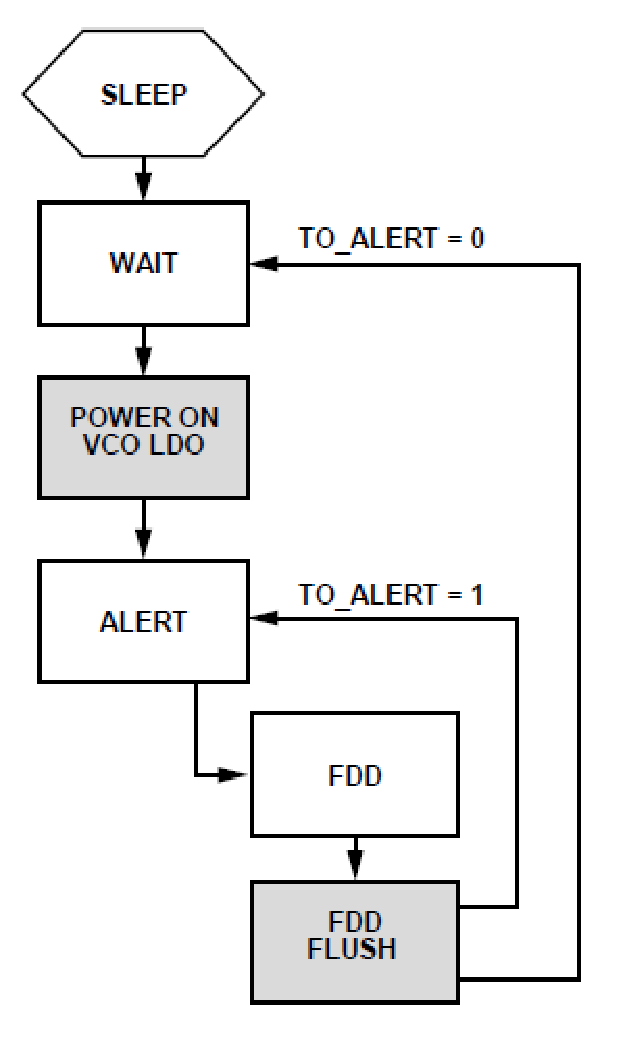
\includegraphics[width=0.25\textwidth]{./figures/fdd_ensm}
    \caption{ FDD Enable State Machine
    \label{fig:pll}}
\end{figure}

\begin{figure}[htbp]
    \centering
    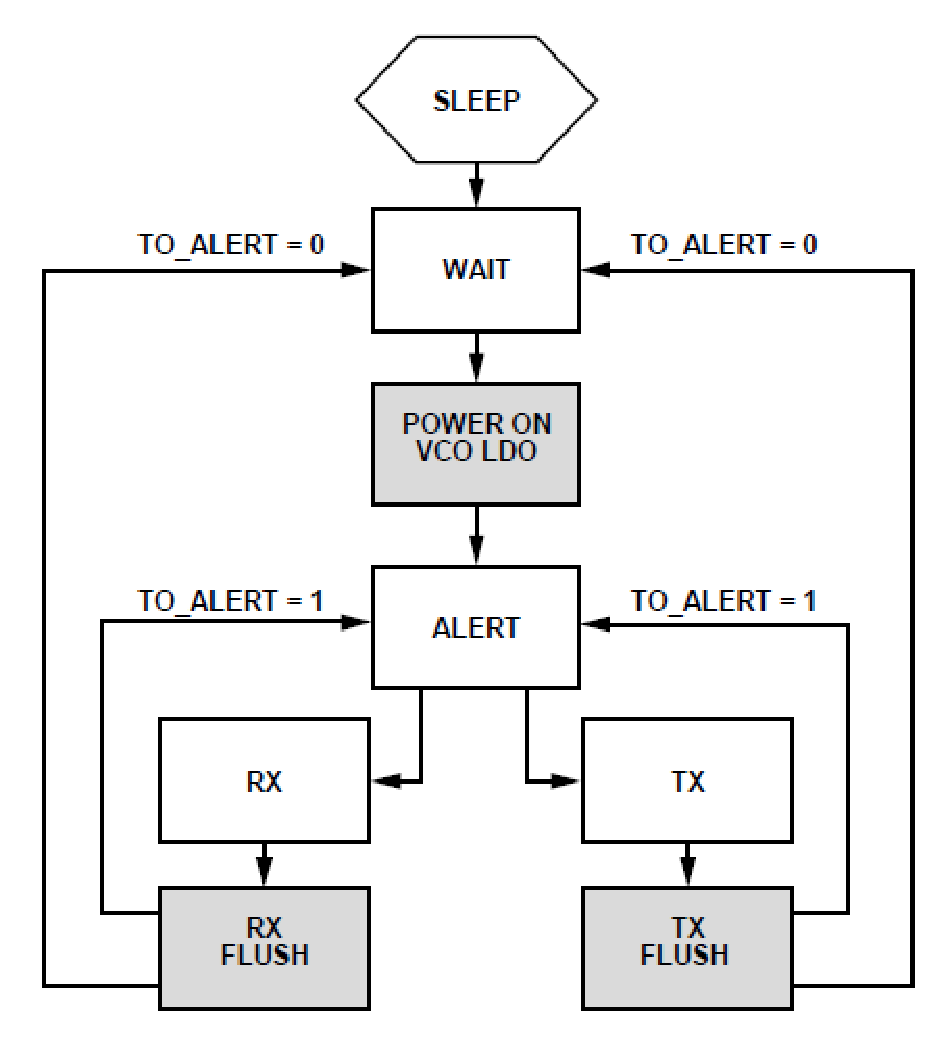
\includegraphics[width=0.35\textwidth]{./figures/tdd_ensm}
    \caption{ TDD Enable State Machine
    \label{fig:pll}}
\end{figure}


\subsubsection{SPI Interface}

The AD9361 uses a SPI interface for communication with the BBP. Throught SPI is
possible to access all the device registers. The PSI interface can be configured
as a 4-wire interface with dedicated transmit and receive pins, duplex, or as
3-wire interface with bidirectional data port. Write commands have a 24-bit
format where the first six bits are for setting the bus direction and number of
bytes to transfer, the next 10 bits set the address where the data is to be
written and the final eight bits are the data to be transferred to the specific
register address (MSB to LSB), a LSB-first format is also supported. Read
commands follow a similar format, the difference is that the first 16 bits are
transferred on the SPI\_DI pin and the final eight are read from the AD9361,
either using SPI\_DO (4-wire interface) or SPI\_DI (3-wire interface).

\subsubsection{Auxiliary Converters}

\begin{description}

	\item[AUXADC] \hfill \\
	The AD(361 contains an auxiliary ADC that can be used to monitor some system
functions such as temperature or power output, it is a 12-bit converter and has
an input range of 0V to 1.25V. The SPI can read the last value latched at the
output of the ADC when it is enabled for use, there is also a multiplexer that
permits to select between AUXADC and built-in temperature sensor.

	\item[AUXDAC1 and AUXDAC2] \hfill \\
	The AD9361 also has two identical auxiliary DACs which can be used to provide
power amplifier (PA) bias or other system functionality. Both the DACs are
10-bit wide and have an output range of 0.5 V to 0.3V and have a current drive
of 10mA. The DACs can be directly controlled by the ENSM.
\end{description}

\subsubsection{Applications}


\subsection{FMCommS2}
\label{subsec:fmcomms2}

FMCommS2 is basically evaluation board for the AD9361 that has a FPGA Mezzanine
Card (FMC) connector for interfacing with the BBP (Usually FPGA). The FMComms2
has 5 SMA connectors, 2 for Rx, 2 for Tx and one for external reference clock
input. The FMComms2 provides a 2x2 RF configuration, extended from the AD9361,
and has  a narrow tuning range balun, which is performance optimized for 2.4GHz.

The FMComms2 is a transceiver intended for use in RF applications such 3G or 4G
BTS or SDR. Its programmability and wideband capability make it ideal for broad
range of transceiver applications and make it very attractive for the new C-RAN
paradigm.

\begin{figure}[htbp]
    \centering
    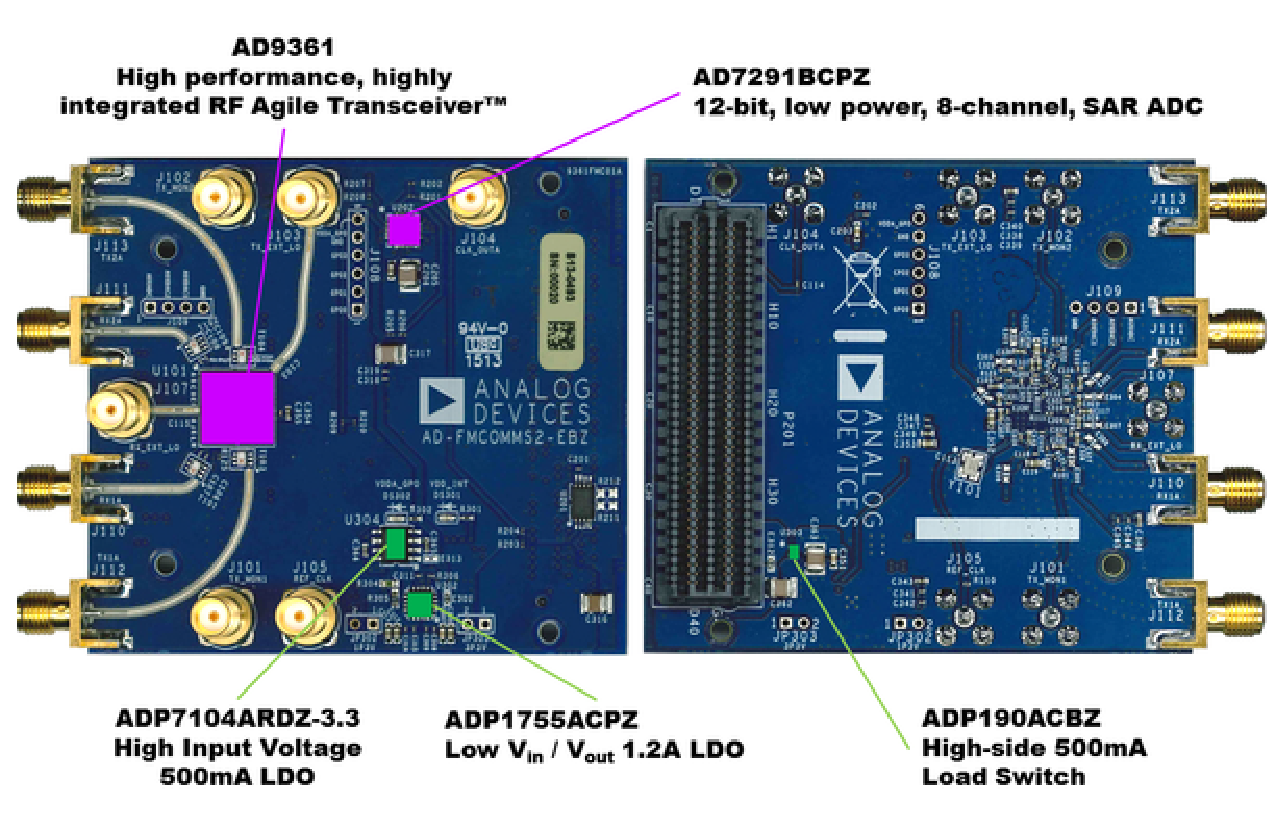
\includegraphics[width=0.65\textwidth]{./figures/fmcomms2_pic}
    \caption{ FMComms2 and its components
    \label{fig:fmcomm}}
\end{figure}


\subsubsection{Functional Overview}

The Block diagram show that there are 4 main functional partitions - receiver
path, transmit path, clocking and power supply. Since the FMComms2 incorporates
and extends the basic functionalities of the AD9361, thus the data path is fully
integrated into the AD9361.

\begin{figure}[htbp]
    \centering
    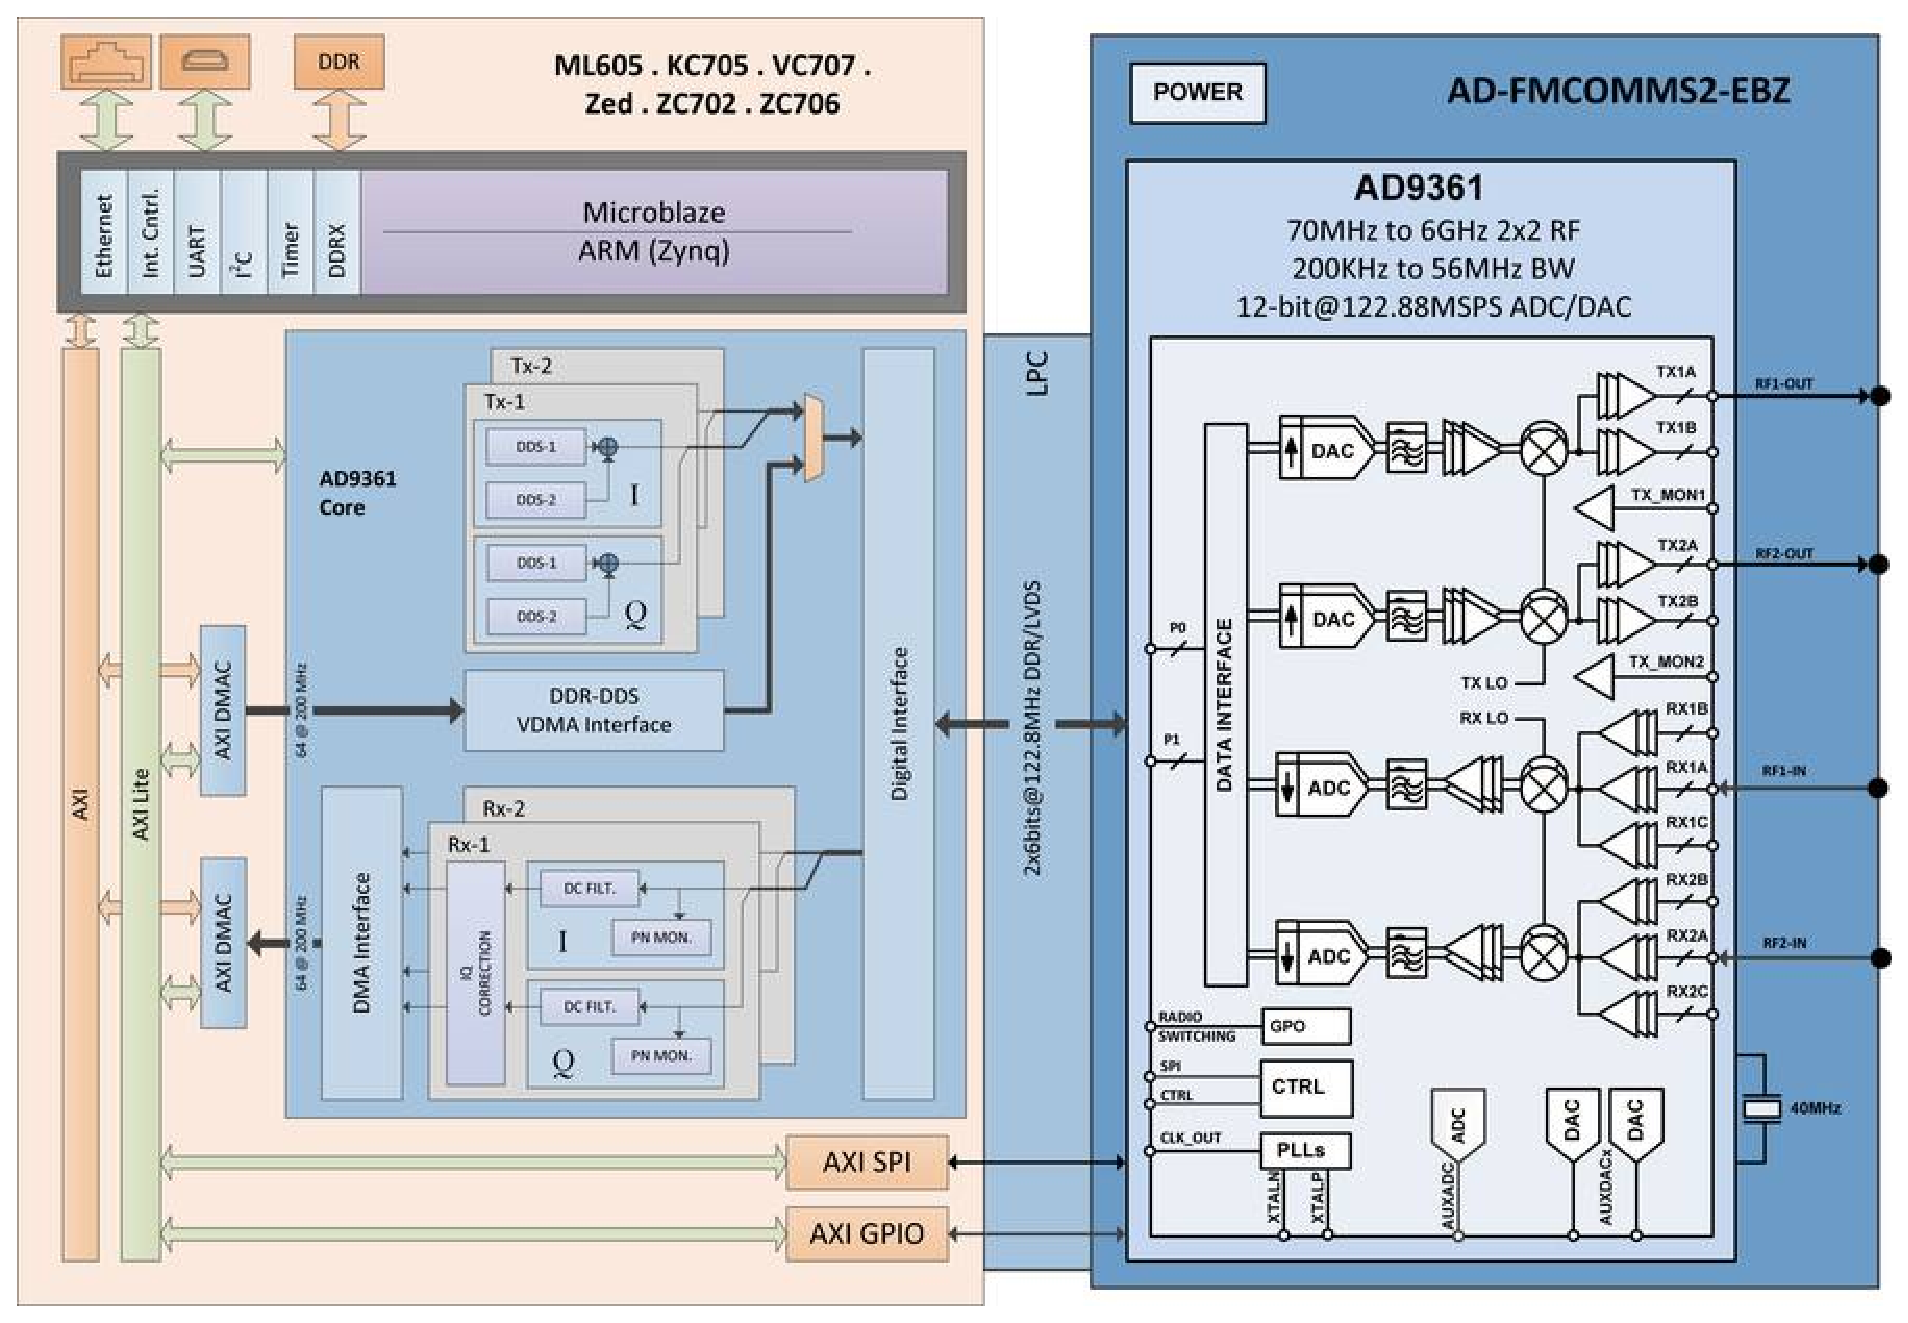
\includegraphics[width=0.65\textwidth]{./figures/fmcomms2_bd}
    \caption{ FMComms2 and FPGA Block Diagram
    \label{fig:fmcommbd}}
\end{figure}



\begin{description}
	\item[Receive] \hfill \\
	\begin{itemize}
		\item Support up to 2 direct conversion RF receiver channels.
		\item Fully integrated frequency synthesizers (including loop filter).
		\item Data path consists in LNA, Demodulator, LPF, ADC and digital filters.
		\item \textit{AGC:} quadrature calibration and DC offset calibration.
		\item \textit{NF:} 2.5 dB at 1Ghz.
		\item \textit{ADC:} Continuous time sigma-delta ( $\Sigma - \Delta$), 640 MSPS.
		\item \textit{Digital Filter:} 128 COmplex taps with decimation between 2 and 48.
		\item \textit{Gain:} 1dB step size, 80 dB analog Range, 30 db digital range (post ADC scaling).
		\item On-chip sensor for temperature corrected RSSI.
	\end{itemize}

	\item[Transmit] \hfill \\
\begin{itemize}
		\item Supports up to 2 direct conversion RF transmit channels.
		\item Fully integrated frequency synthesizers (including loop filter).
\item Data path consists of digital filters, DAC and modulators.
		\item \textit{Digital Filter:} 128 complex taps with interpolation between 2 and 48.
		\item \textit{Gain:} 0.5 dB step size, 86 dB range.
		\item \textit{ADC:} 340 MSPS.
	\end{itemize}

	\item[Clocking] \hfill \\
		The FMComms2 board has a integrated crystal oscillator of 40 Mhz and has a SMA
input for external clock input.

	\item[Control/Monitor] \hfill \\
		The board allows real time control and monitoring via dedicated pins, such pins
functionality are programmable. The control and monitor programming
configuration is specified in the ad9361 section \ref{subsec:ad9361}.

\end{description}

\subsection{Basic Mathematical Background}

\subsubsection{Complex Modulation}

\begin{eqnarray}
	I = sin(\omega \times t)\\
	Q = cos(\omega \times t)
\end{eqnarray}

\begin{equation}
	cos(\omega \times t) = sin(\frac{\pi}{2} - (\omega \times t))
\end{equation}

then:

\begin{eqnarray}
	I = sin(\omega \times t)\\
	Q = sin(\frac{\pi}{2} - (\omega \times t))
\end{eqnarray}

These are the two signals coming out of the DAC, two sine waves, phase offset from each other, wich is called IQ.

\subsubsection{Basic Modulation Mathematics}

Start to modulating signal from a amplitude perspective:

\begin{eqnarray}
LO_I = A_x cos(k)\\
LO_Q = B_x sin(k)
\end{eqnarray}

We still have the carrier:

\begin{equation}
LO_I = cos(\omega) ; LO_Q = sin(\omega)
\end{equation}

Will result:

\begin{eqnarray}
LO_I \times I = A_x cos(k) \times sin(\omega)\\
LO_Q \times I = B_x sin(k) \times cos(\omega)
\end{eqnarray}


That gives the output:

\begin{equation}
x(t)=A_x cos(k)\times sin(\omega)+ B_x sin(k)\times cos(\omega)
\end{equation}

This does not match with any trigonometrical identities and it is easier to use Euler\'s formula:

\begin{eqnarray}
sin(x)=(\frac{1}{2}e^{-jx} - \frac{1}{2}e^{jx})\\
cos(x)=(\frac{1}{2}e^{-jx} + \frac{1}{2}e^{jx})
\end{eqnarray}

Therefore:

\begin{equation}
x(t)=A_x (\frac{1}{2}e^{-jk} + \frac{1}{2}e^{jk})\times (\frac{1}{2}e^{-j\omega} - \frac{1}{2}e^{j\omega})+ B_x (\frac{1}{2}e^{-jk} - \frac{1}{2}e^{jk})\times (\frac{1}{2}e^{-j\omega} + \frac{1}{2}e^{j\omega})
\end{equation}

\begin{equation}
x(t)=\frac{A}{2} (e^{-jk} + e^{jk})\times (e^{-j\omega} - e^{j\omega})+ \frac{B}{2} (e^{-jk} - e^{jk})\times (e^{-j\omega} + e^{j\omega})
\end{equation}

If we expand we get:

\begin{equation}
x(t)=\frac{1}{2} ((Ae^{-jk-j\omega} + Ae^{jk-j\omega} - Ae^{-jk+j\omega} - Ae^{jk+j\omega}) + (Be^{-jk-j\omega} - Be^{jk-j\omega} - Be^{-jk+j\omega} + Be^{jk+j\omega}))
\end{equation}


And then:

\begin{equation}
x(t)=\frac{1}{2} ((A+B)e^{-jk-j\omega} + (A-B)e^{jk-j\omega} - (A-B)e^{-jk+j\omega} - (A+B)e^{jk+j\omega})
\end{equation}

It is possible to rearrange as:

\begin{equation}
x(t)=\frac{1}{2} \times ((A+B)(e^{-jk-j\omega} - e^{jk+j\omega}) + (A-B)(e^{jk-j\omega} - e^{-jk+j\omega}))
\end{equation}

And then:

\begin{equation}
x(t)=(\frac{A+B}{2} )(sin(k+\omega)) + (\frac{A-B}{2} )(sin(k-\omega))
\end{equation}

If this due to amplitude mismatch, this creates an image on the other side of
the local oscillator.

\section{Setup}
\label{impl:setup}

\subsection{Overview}

As stated before, C-RAN is still in development and it is not already a solid
standard, so exploring setups and their feasibility is very interesting to
increase the ways to implement this new standard in countries which does not
have a very good infrastructure.

The first setup thought was using the ML605 FMC LPC connector and the FMComms2,
this setup was very important because in it I could understand how to integrate
the board design with the need of the project. Then the device was moved to the
FMC HPC connector and the design with the ML605 was finished.

After getting the experience with ML605 and ISE design tools, it was time to use
a more updated board and design tool, thus the idea of porting the initial
design from ML605 to the VC707 board came. Since ISE has no support for VC707
and is a software with its development halted, going to the most updated tool
from Xilinx is natural, so the second setup is using vivado design tools and
VC707 with FMC HPC connector and FMComms2.

Another thing to give attention is that with ISE the design flow was more manual
and if there was the need to rebuild a project almost from the scratch, just
with the HDL source files, the other necessary ips should be created and
configured again, which took a lot of time, but with Vivado the block diagram
design flow and the .tcl scripts became more popular, they existed in ISE
however they were not popular. With the TCL scripts it is possible to create
project, import files, instantiate and configure both user and default IPs, as
well as run synthesis, implementation and generate bitstream steps, which saves
a lot of time in development.

%figura do setup com diagrama de blocos
\begin{figure}[htbp]
    \centering
    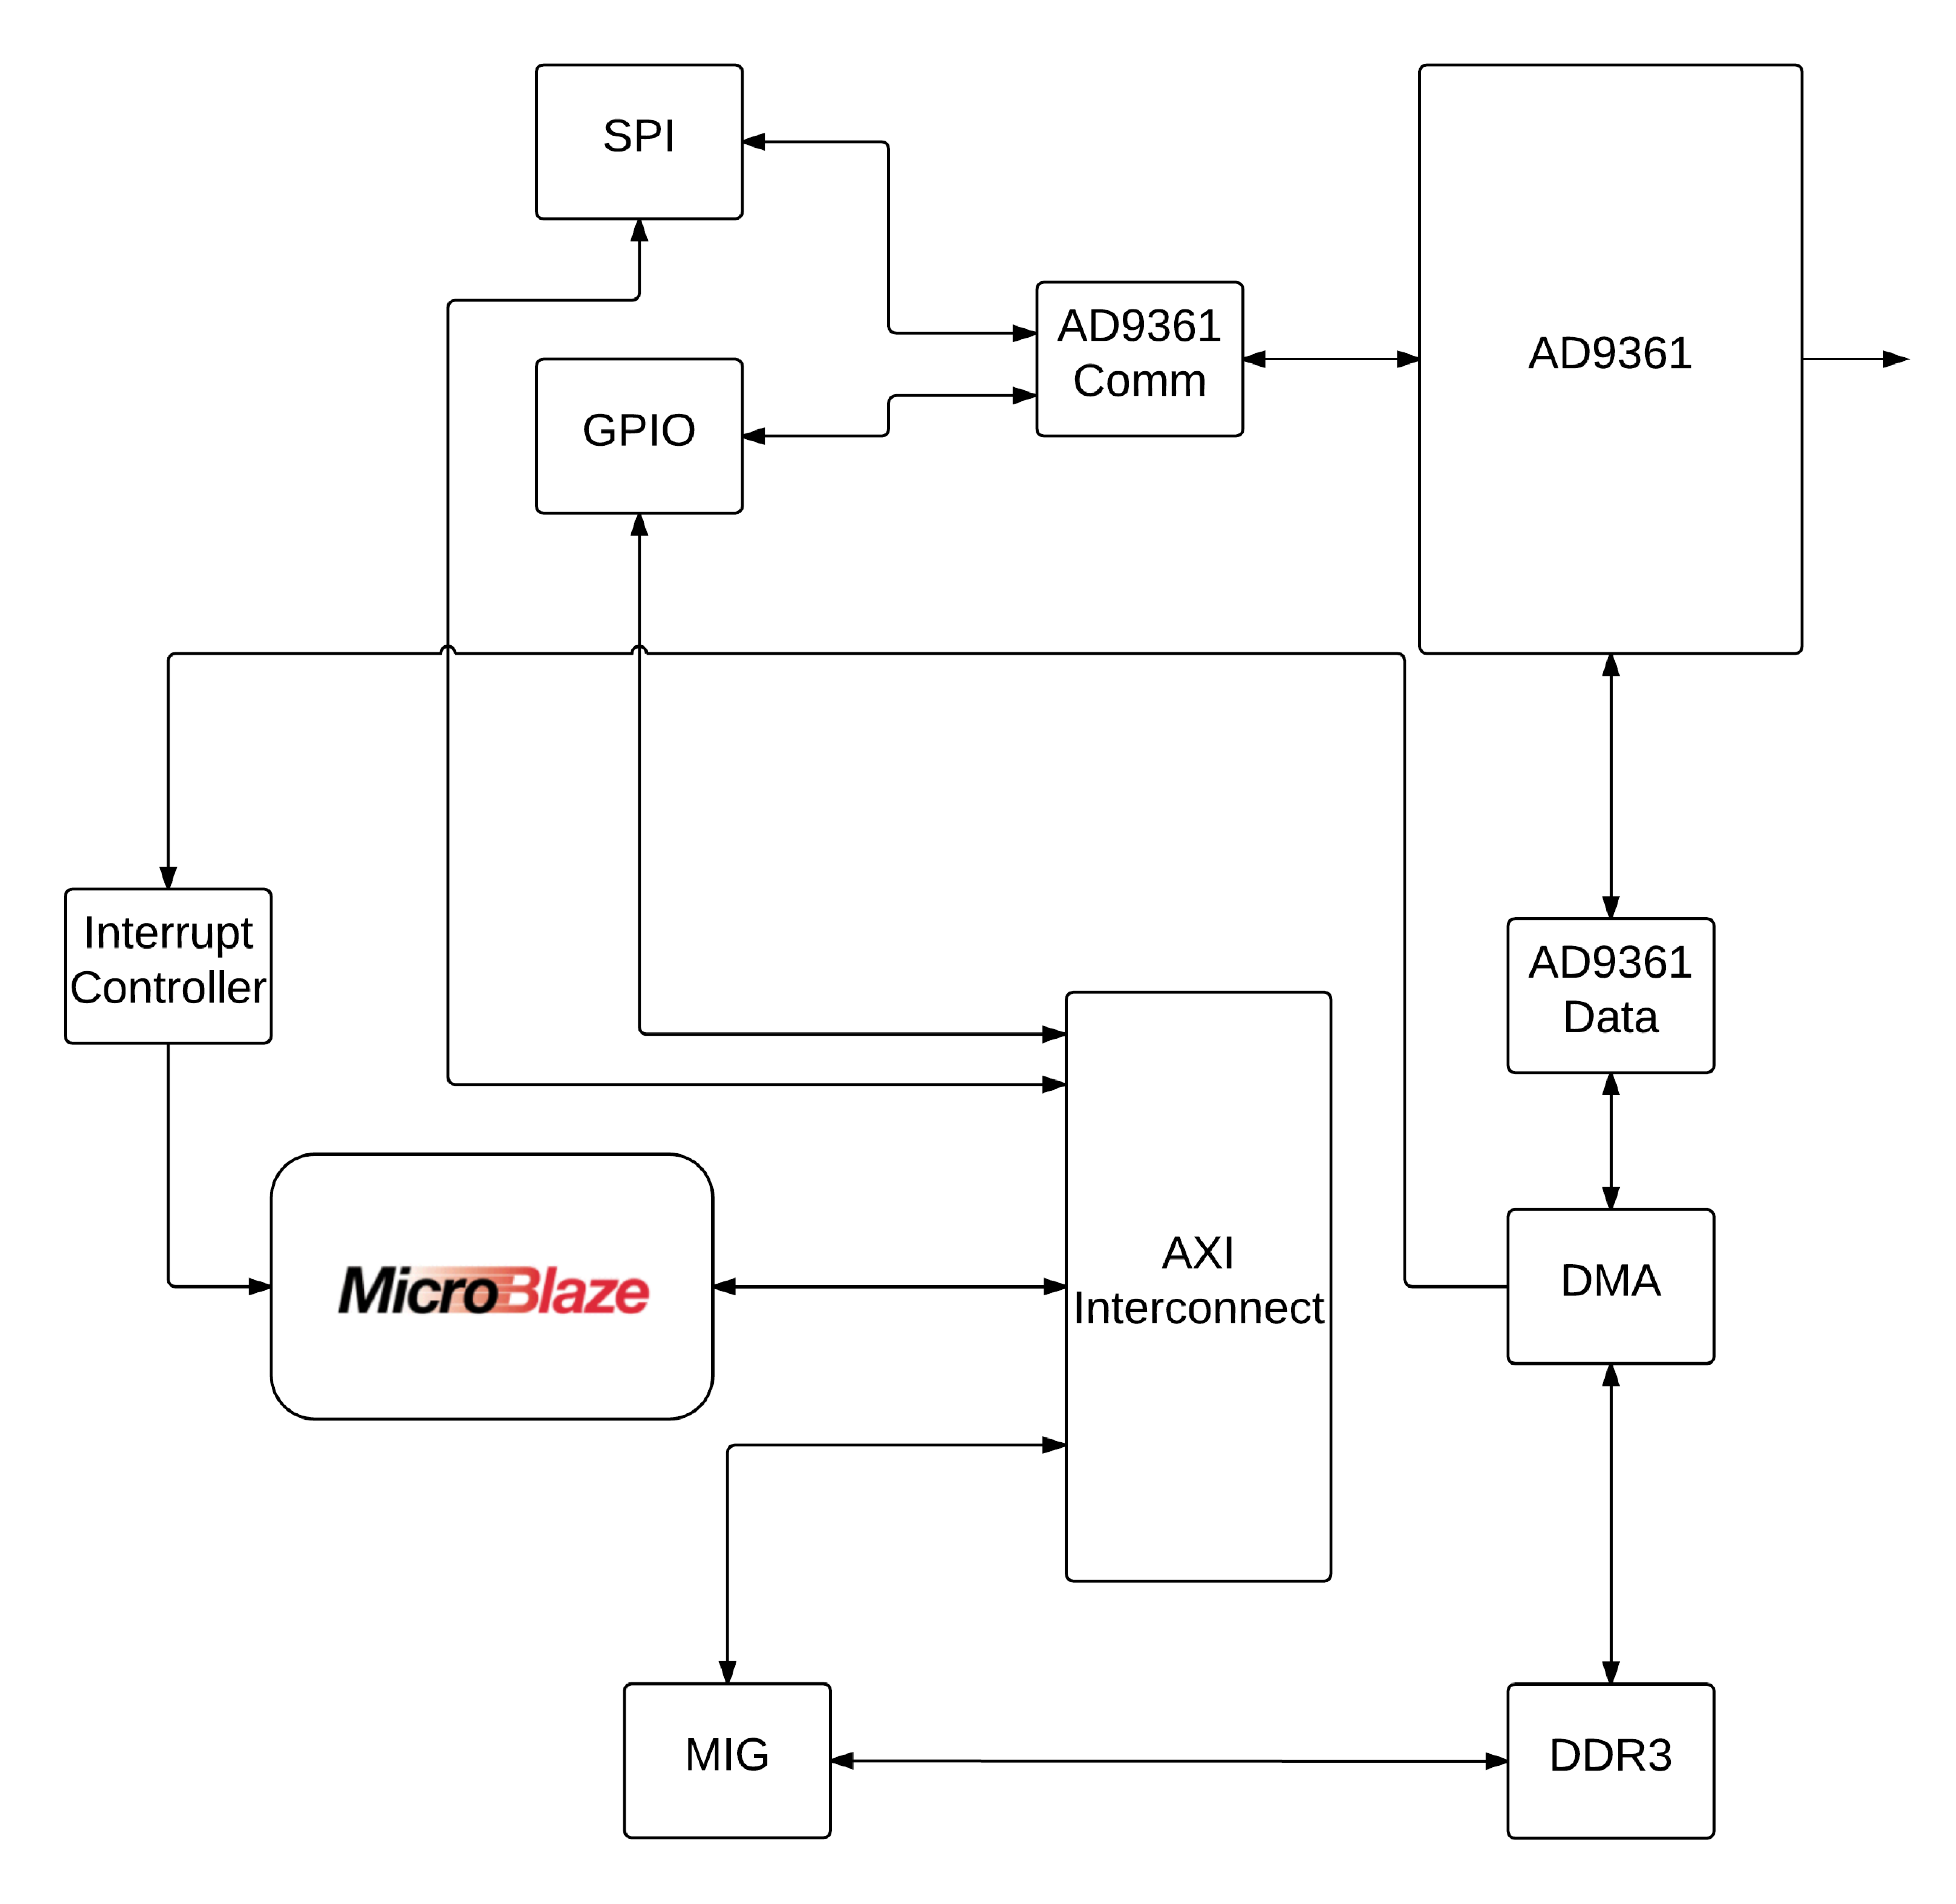
\includegraphics[width=0.65\textwidth]{./figures/setup_ipbd}
    \caption{ Setup Components block diagram
    \label{fig:setupip}}
\end{figure}

\subsection{Integration between FPGA and FMComms2}

The first problem encountered in the development was the integration, since the
company make a example project available and the IP cores for download it appear
to be an easy job, however, for study purposes and for a simpler design it is
better to begin a bottom up approach and so it was did.

This approach was used in both ML605 and VC707 and it consists in basic steps:

\begin{enumerate}
    \item Analyse which ports have to be connected
    \item Analyse which Communications protocols are needed to communicate with the device;
    \item Analyse the clock inputs and give the device the clocks it need to properly work;
    \item Study both the HDL sources and the Driver to understand how the device works.
\end{enumerate}

This analyze work took around 3 weeks and the the integration became to work
properly. In the ML605 the version of the IP and driver was one of the first
ones, then it was needed only the SPI for registers read and write and one
GPIO pin to reset the device.

By default the AD9361 driver has a DDS which generates the carrier wave at 2.4Ghz,
so if the initialization work it is possible to watch in the oscilloscope or
spectrum analyzer a sinusoidal (Carrier) wave at 2.4 Ghz after all initialization
procedures have been done.

\subsection{Control Interface}
\label{subs:controlif}

As stated in the previous subsection the FMComms2 control and communication
interface is implemented through GPIO pins and SPI protocol, basically SPI is
used to write and read registers in the board while GPIO is used for real-time
control, like reset or change states in the ENSM.

While the development was in its beginning the minimum pins for communication
and reset work were assigned, however when the development wen to Vivado with
the VC707 there was the need to build something more automated in order to be
easily rebuild, so the \emph{ad9361\_comm} IP was created to route the respective
pins from SPI and GPIO interfaces to the ad9361 control and communication interface.

Below it is possible to see in a simple schematic what is the \emph{ad9361\_comm}
IP and how it routes the respective ports to the ad9361 interface.

%diagrama de blocos control interface
\begin{figure}[htbp]
    \centering
    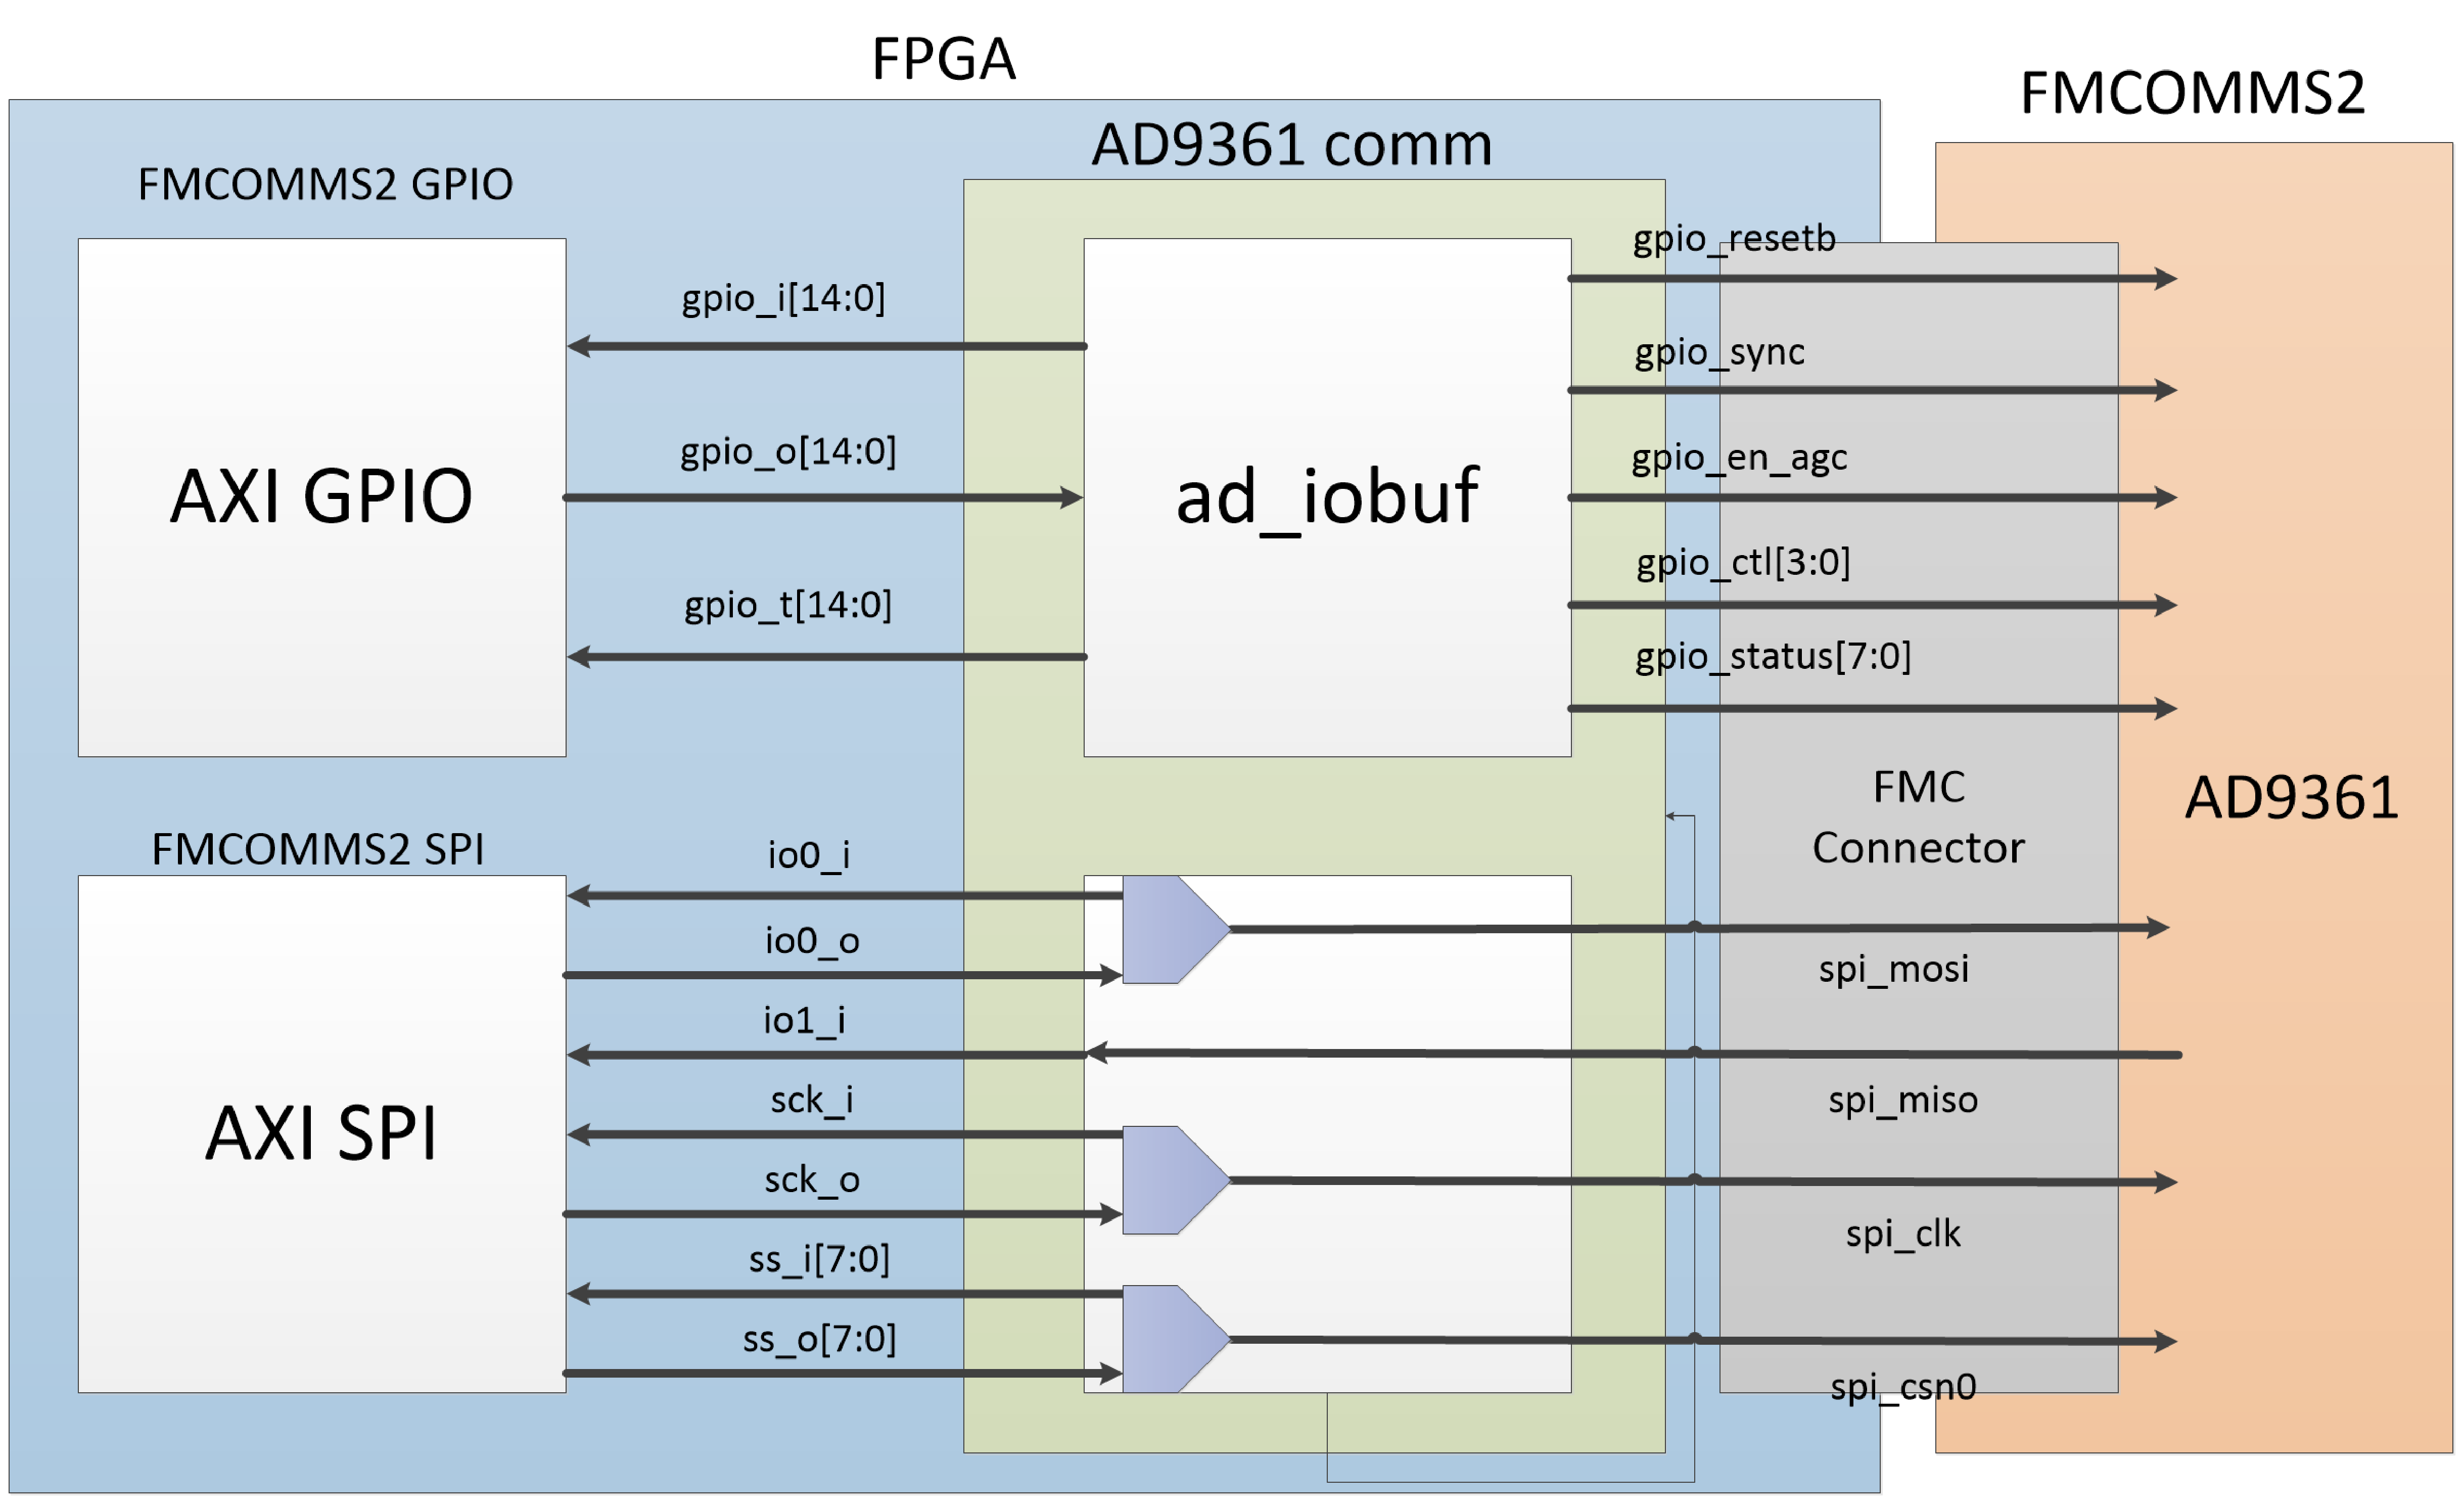
\includegraphics[width=0.65\textwidth]{./figures/comm_if}
    \caption{ Control Interface Block Diagram
    \label{fig:commif}}
\end{figure}

\subsection{Transmitting custom data}

After having the communication and initialization between FPGA and FMComms2
board working properly, the next step was to input custom data into the device
and efficiently transmit modulated information in the carrier wave.

There is two basic ways to input data into the AD9361, to do so it is necessary to understand
its communication interface, which is similar to the axi-stream interface with
3 ports, one for data, one for enable and one for valid. The first approach for
input data into the transceiver was use a FIFO with a DDS IP in the FPGA, which
is not so fast and reliable, but it was enough for test purposes.

%inserir figura do IP ad9361 highlight TX interface pins
\begin{figure}[htbp]
    \centering
    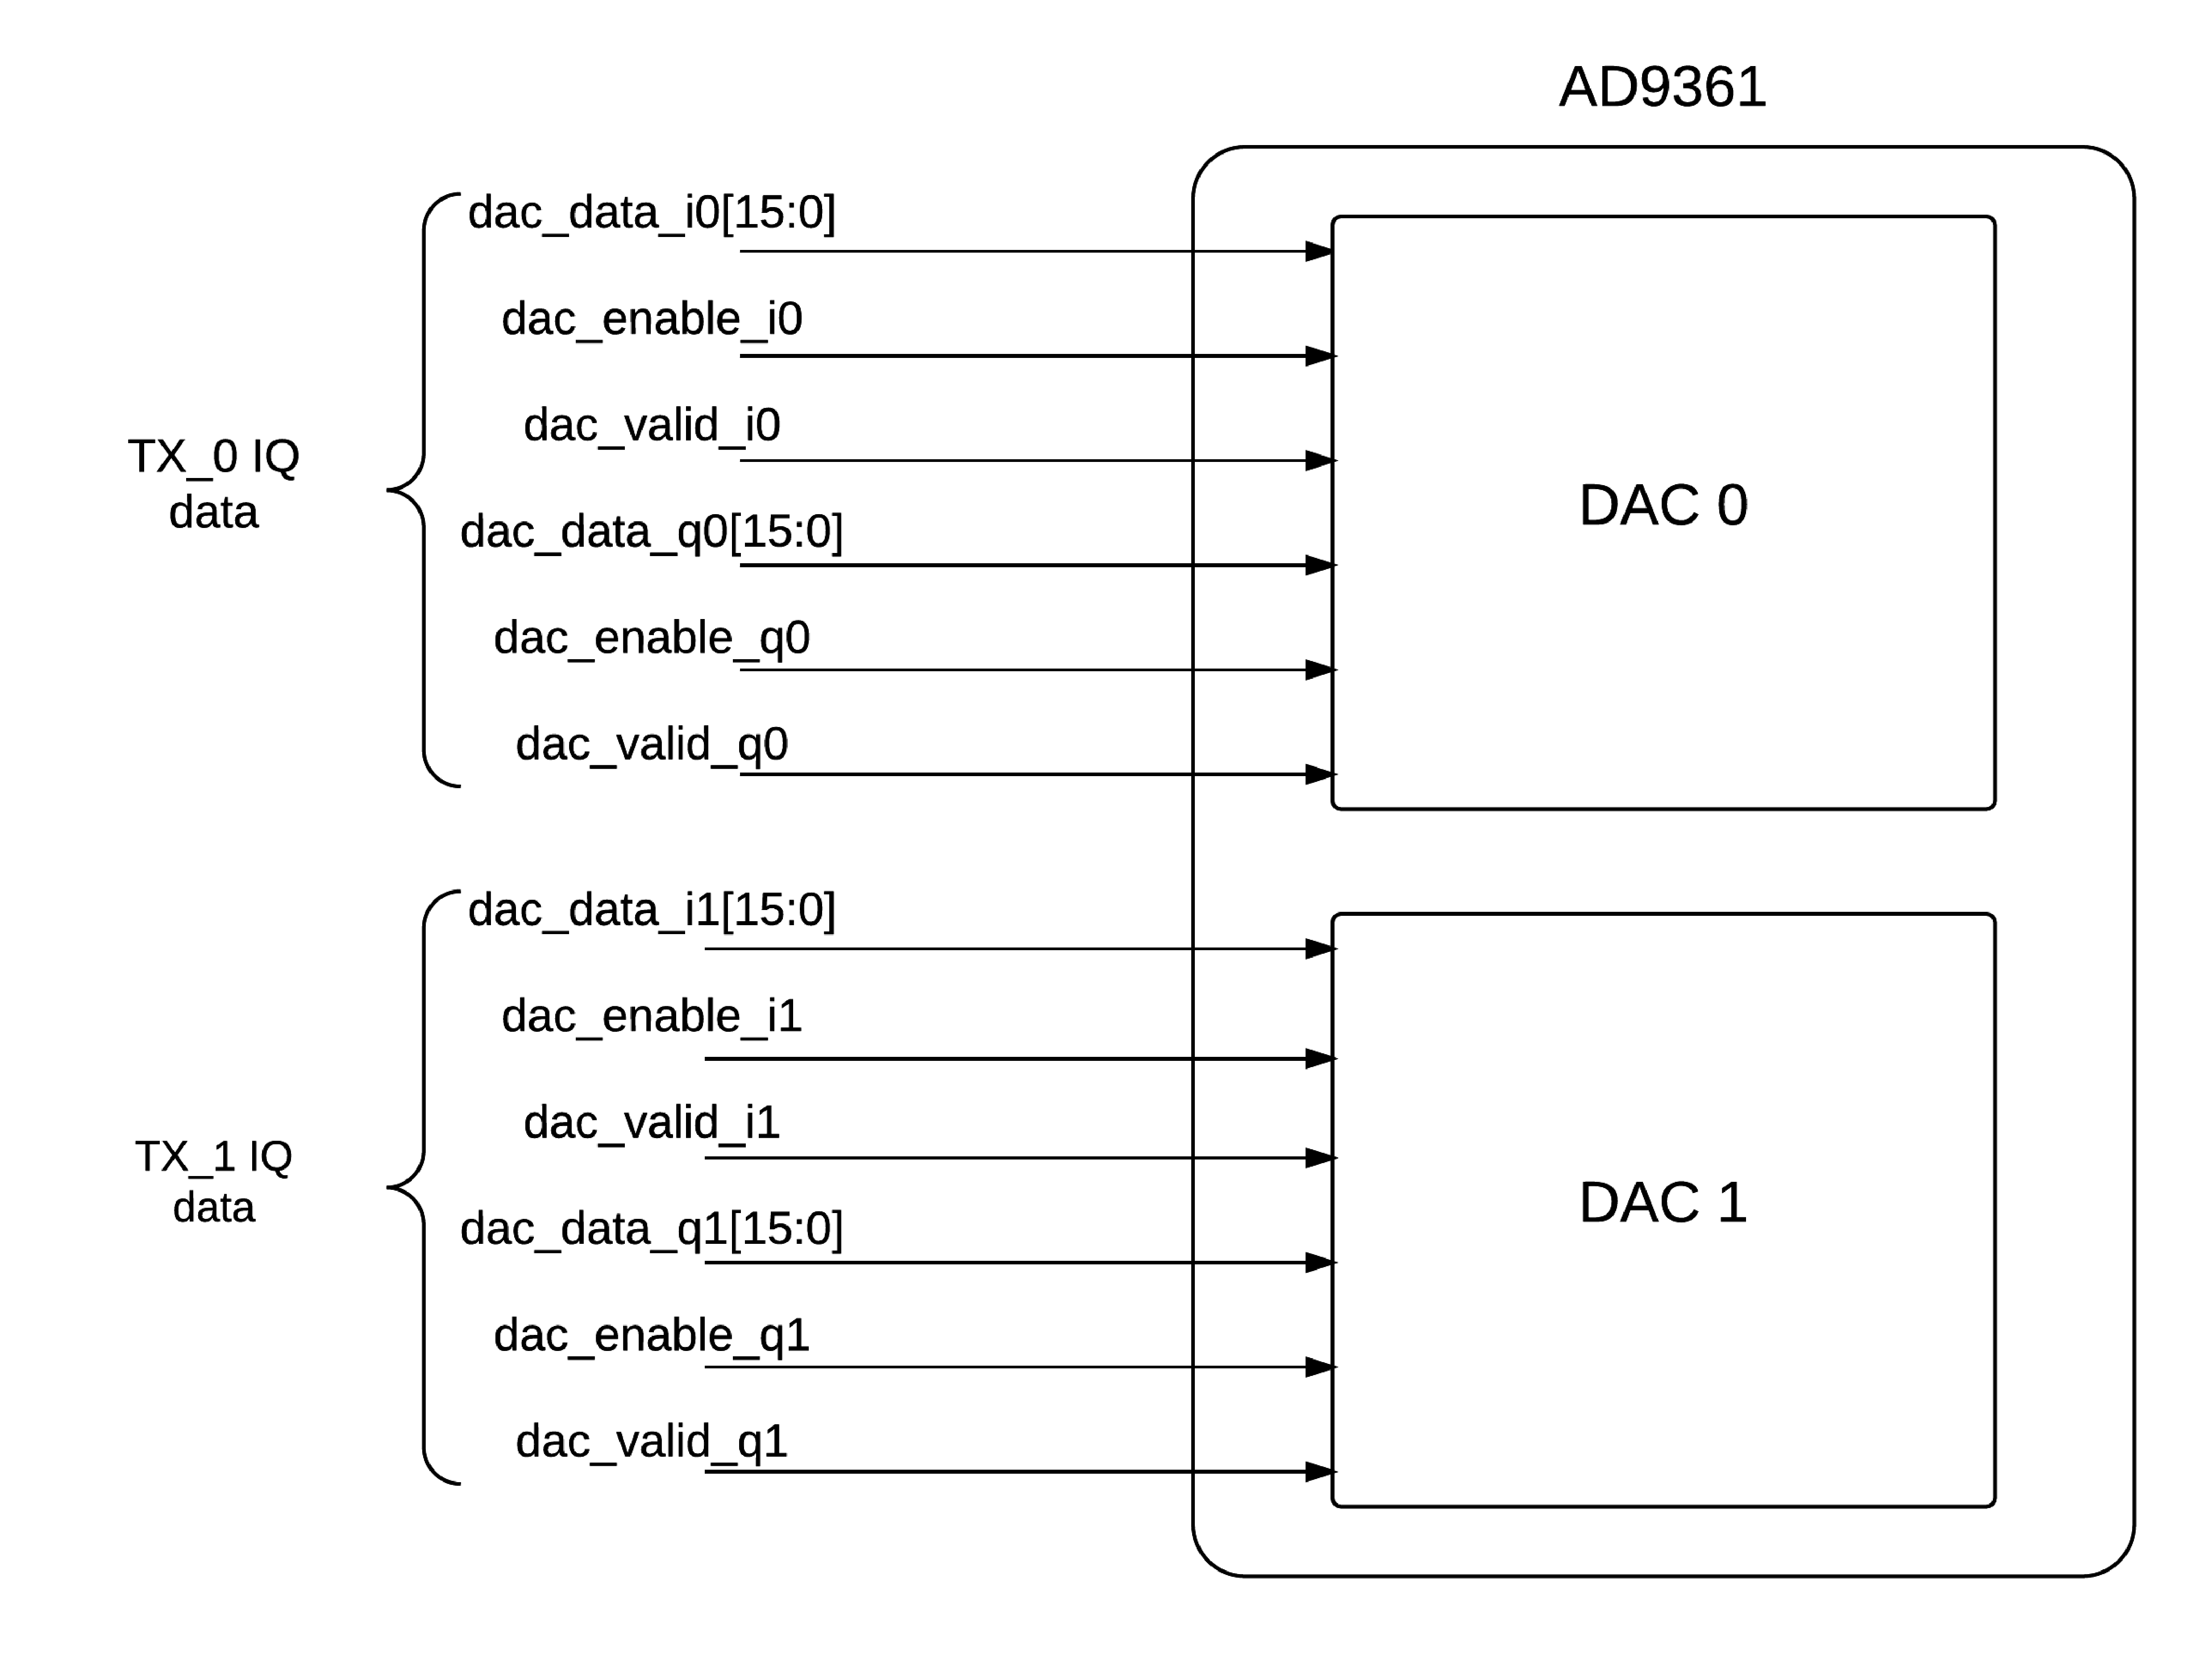
\includegraphics[width=0.65\textwidth]{./figures/ad9361tx_pins}
    \caption{ AD9361 Transmitter (DAC) interface pins
    \label{fig:txpins}}
\end{figure}

%inserir diagrama de blocos de entrada DDS>FIFO>AD9361

\begin{figure}[htbp]
    \centering
    
\includegraphics[width=0.65\textwidth]{./figures/dac_fifo}
    \caption{ ad9361 DAC interface with FIFO
    \label{fig:ad9361txfifo}}
\end{figure}

After some time, the need for a faster interface rose, then the use of DMA came
naturally, because it is faster and more reliable than the common FIFO.

%inserir figura da interface DMA>AD9361
\begin{figure}[htbp]
    \centering
    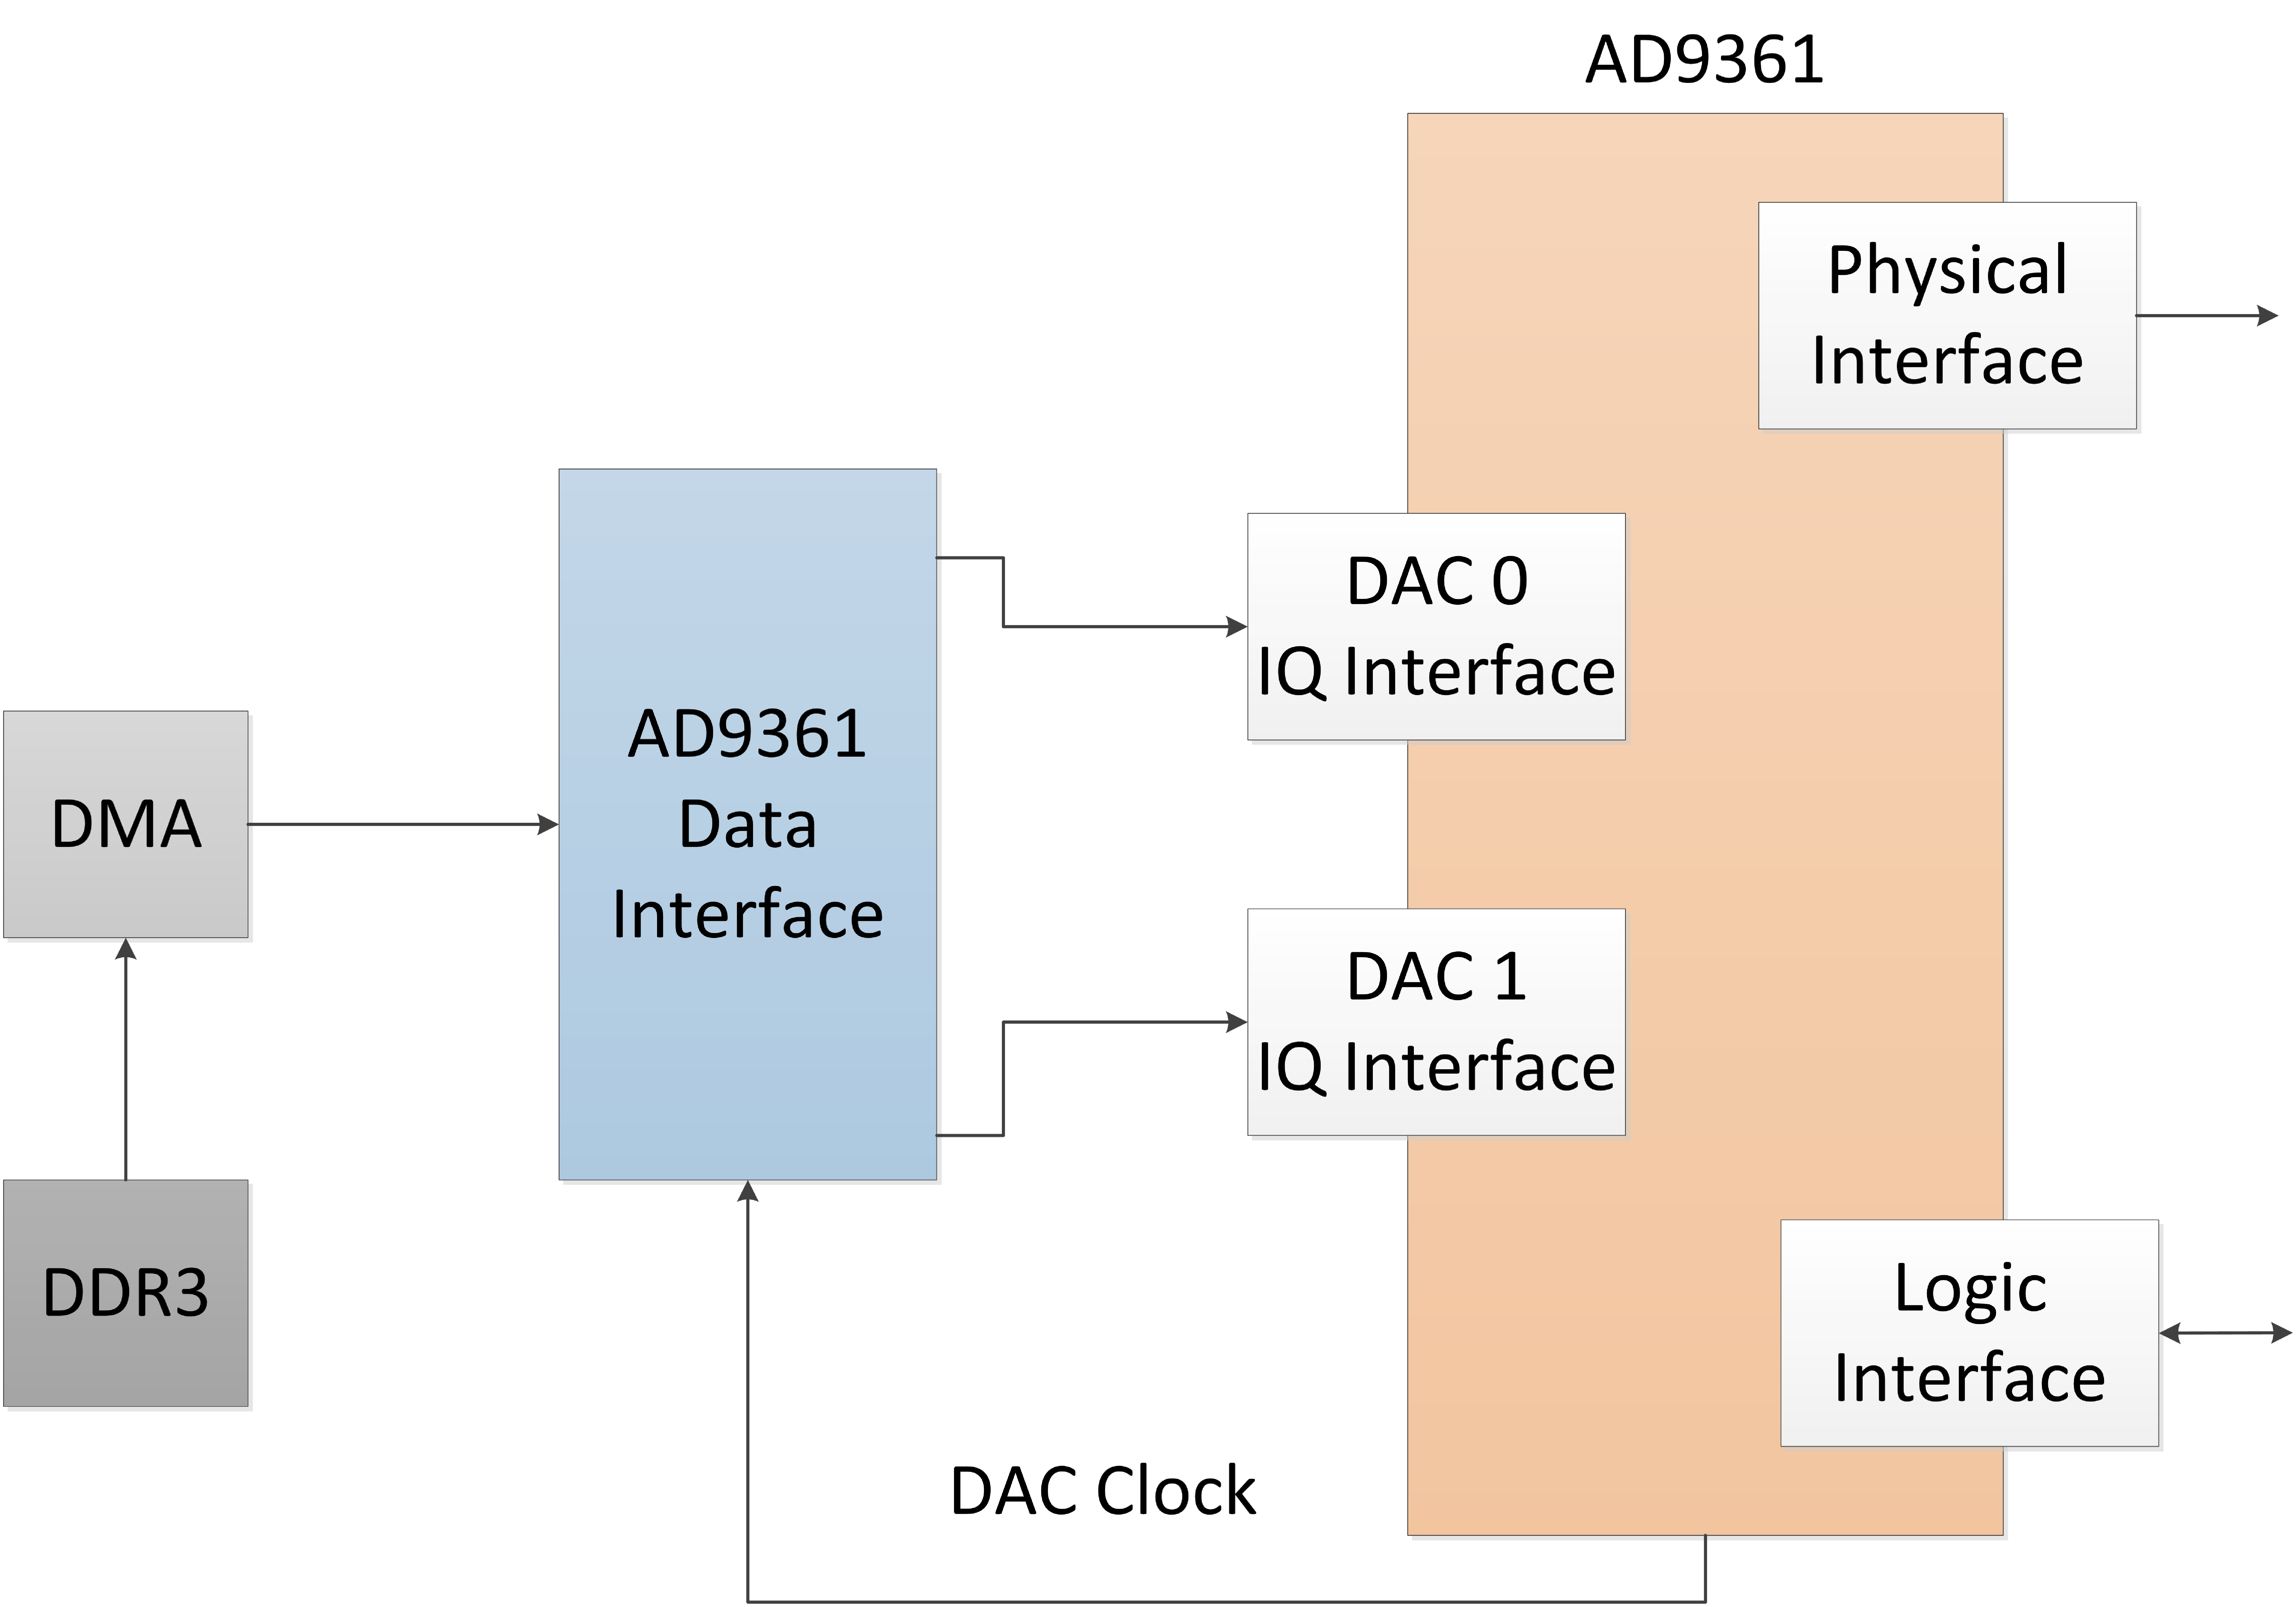
\includegraphics[width=0.65\textwidth]{./figures/dac_dma}
    \caption{ ad9361 DAC interface with DMA
    \label{fig:ad9361txdma}}
\end{figure}

\subsection{Receiving Custom data}

Receiving is the exact opposite of transmitting custom data, in the beginning of
the setup implementation using a DDS IP and a fifo to input IQ data into the
AD9361 was intuitively the easier way for transmission, and indeed was the same
thing for receiving.

%inserir figura do IP ad9361 Highlight RX interface pins
\begin{figure}[htbp]
    \centering
    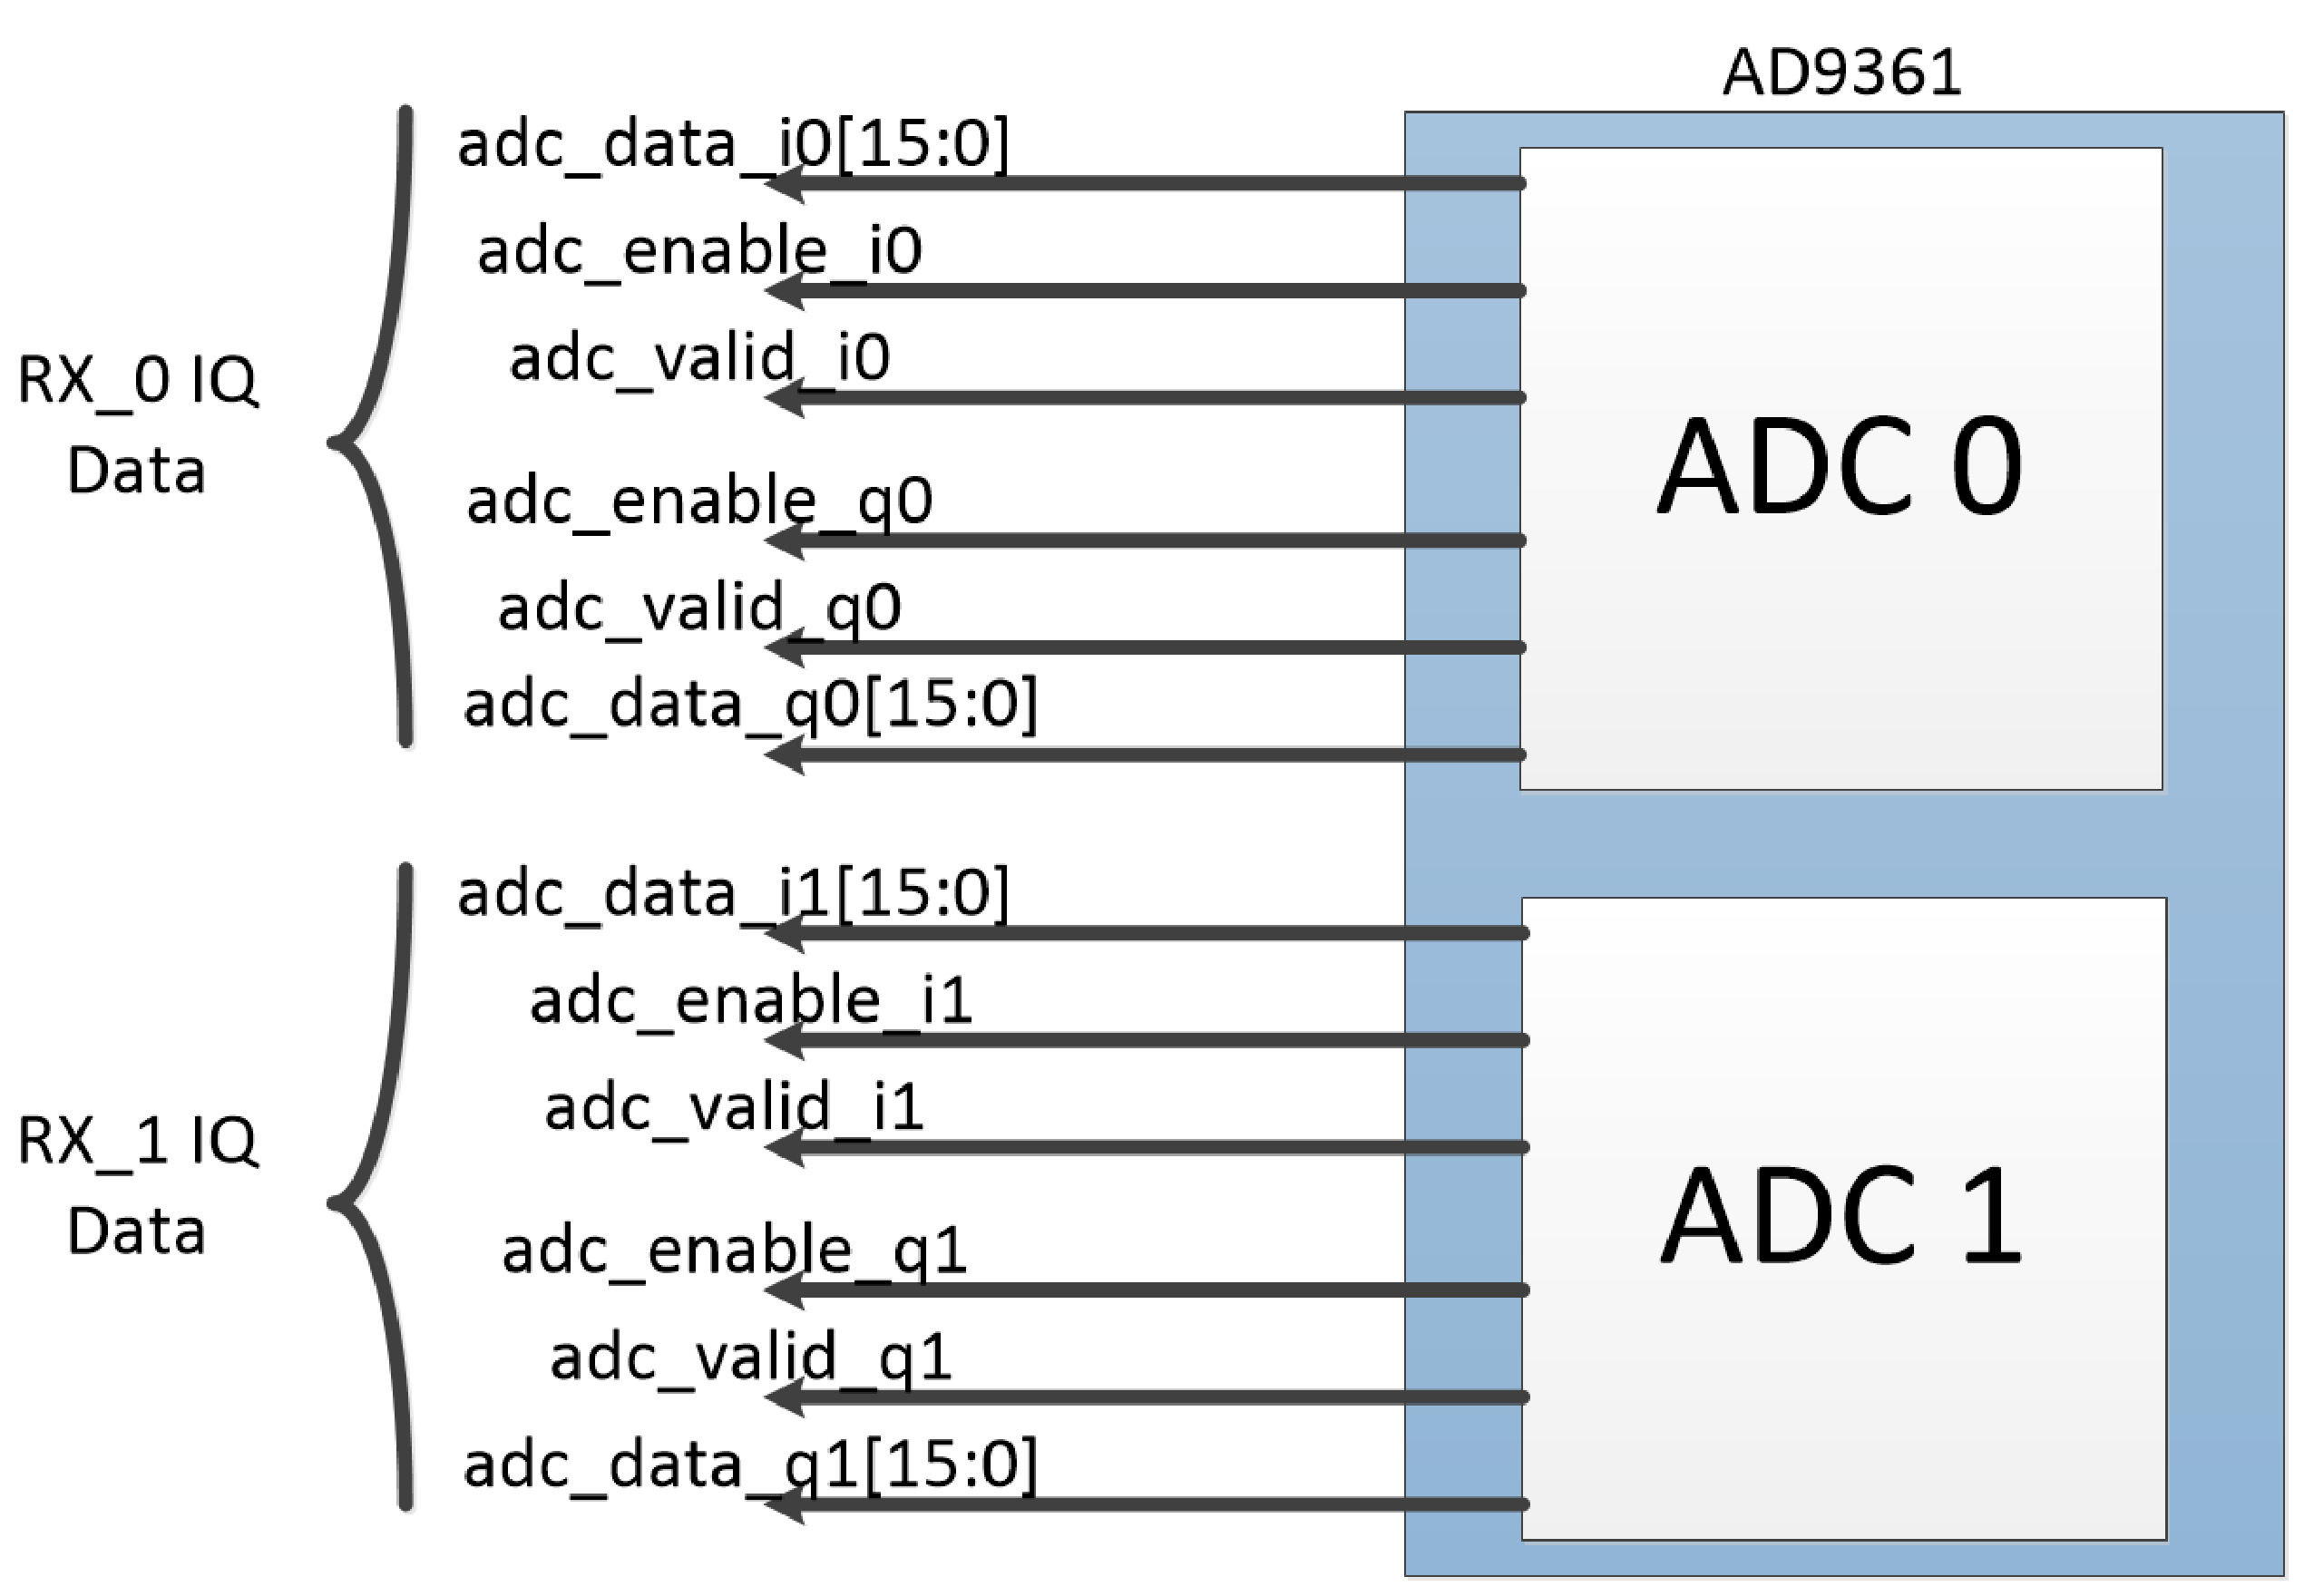
\includegraphics[width=0.65\textwidth]{./figures/ad9361rx_pins}
    \caption{ AD9361 Receiver (ADC) interface pins
    \label{fig:rxpins}}
\end{figure}

%inserir diagrama de blocos de entrada AD9361>FIFO>ILA
\begin{figure}[htbp]
    \centering
    
\includegraphics[width=0.65\textwidth]{./figures/adc_fifo}
    \caption{ ad9361 ADC interface with FIFO
    \label{fig:ad9361rxfifo}}
\end{figure}

The same idea used in transmission when the VC707 development began was applied
to the receiver, use DMA.

%inserir figura da interface AD9361>DMA
\begin{figure}[htbp]
    \centering
    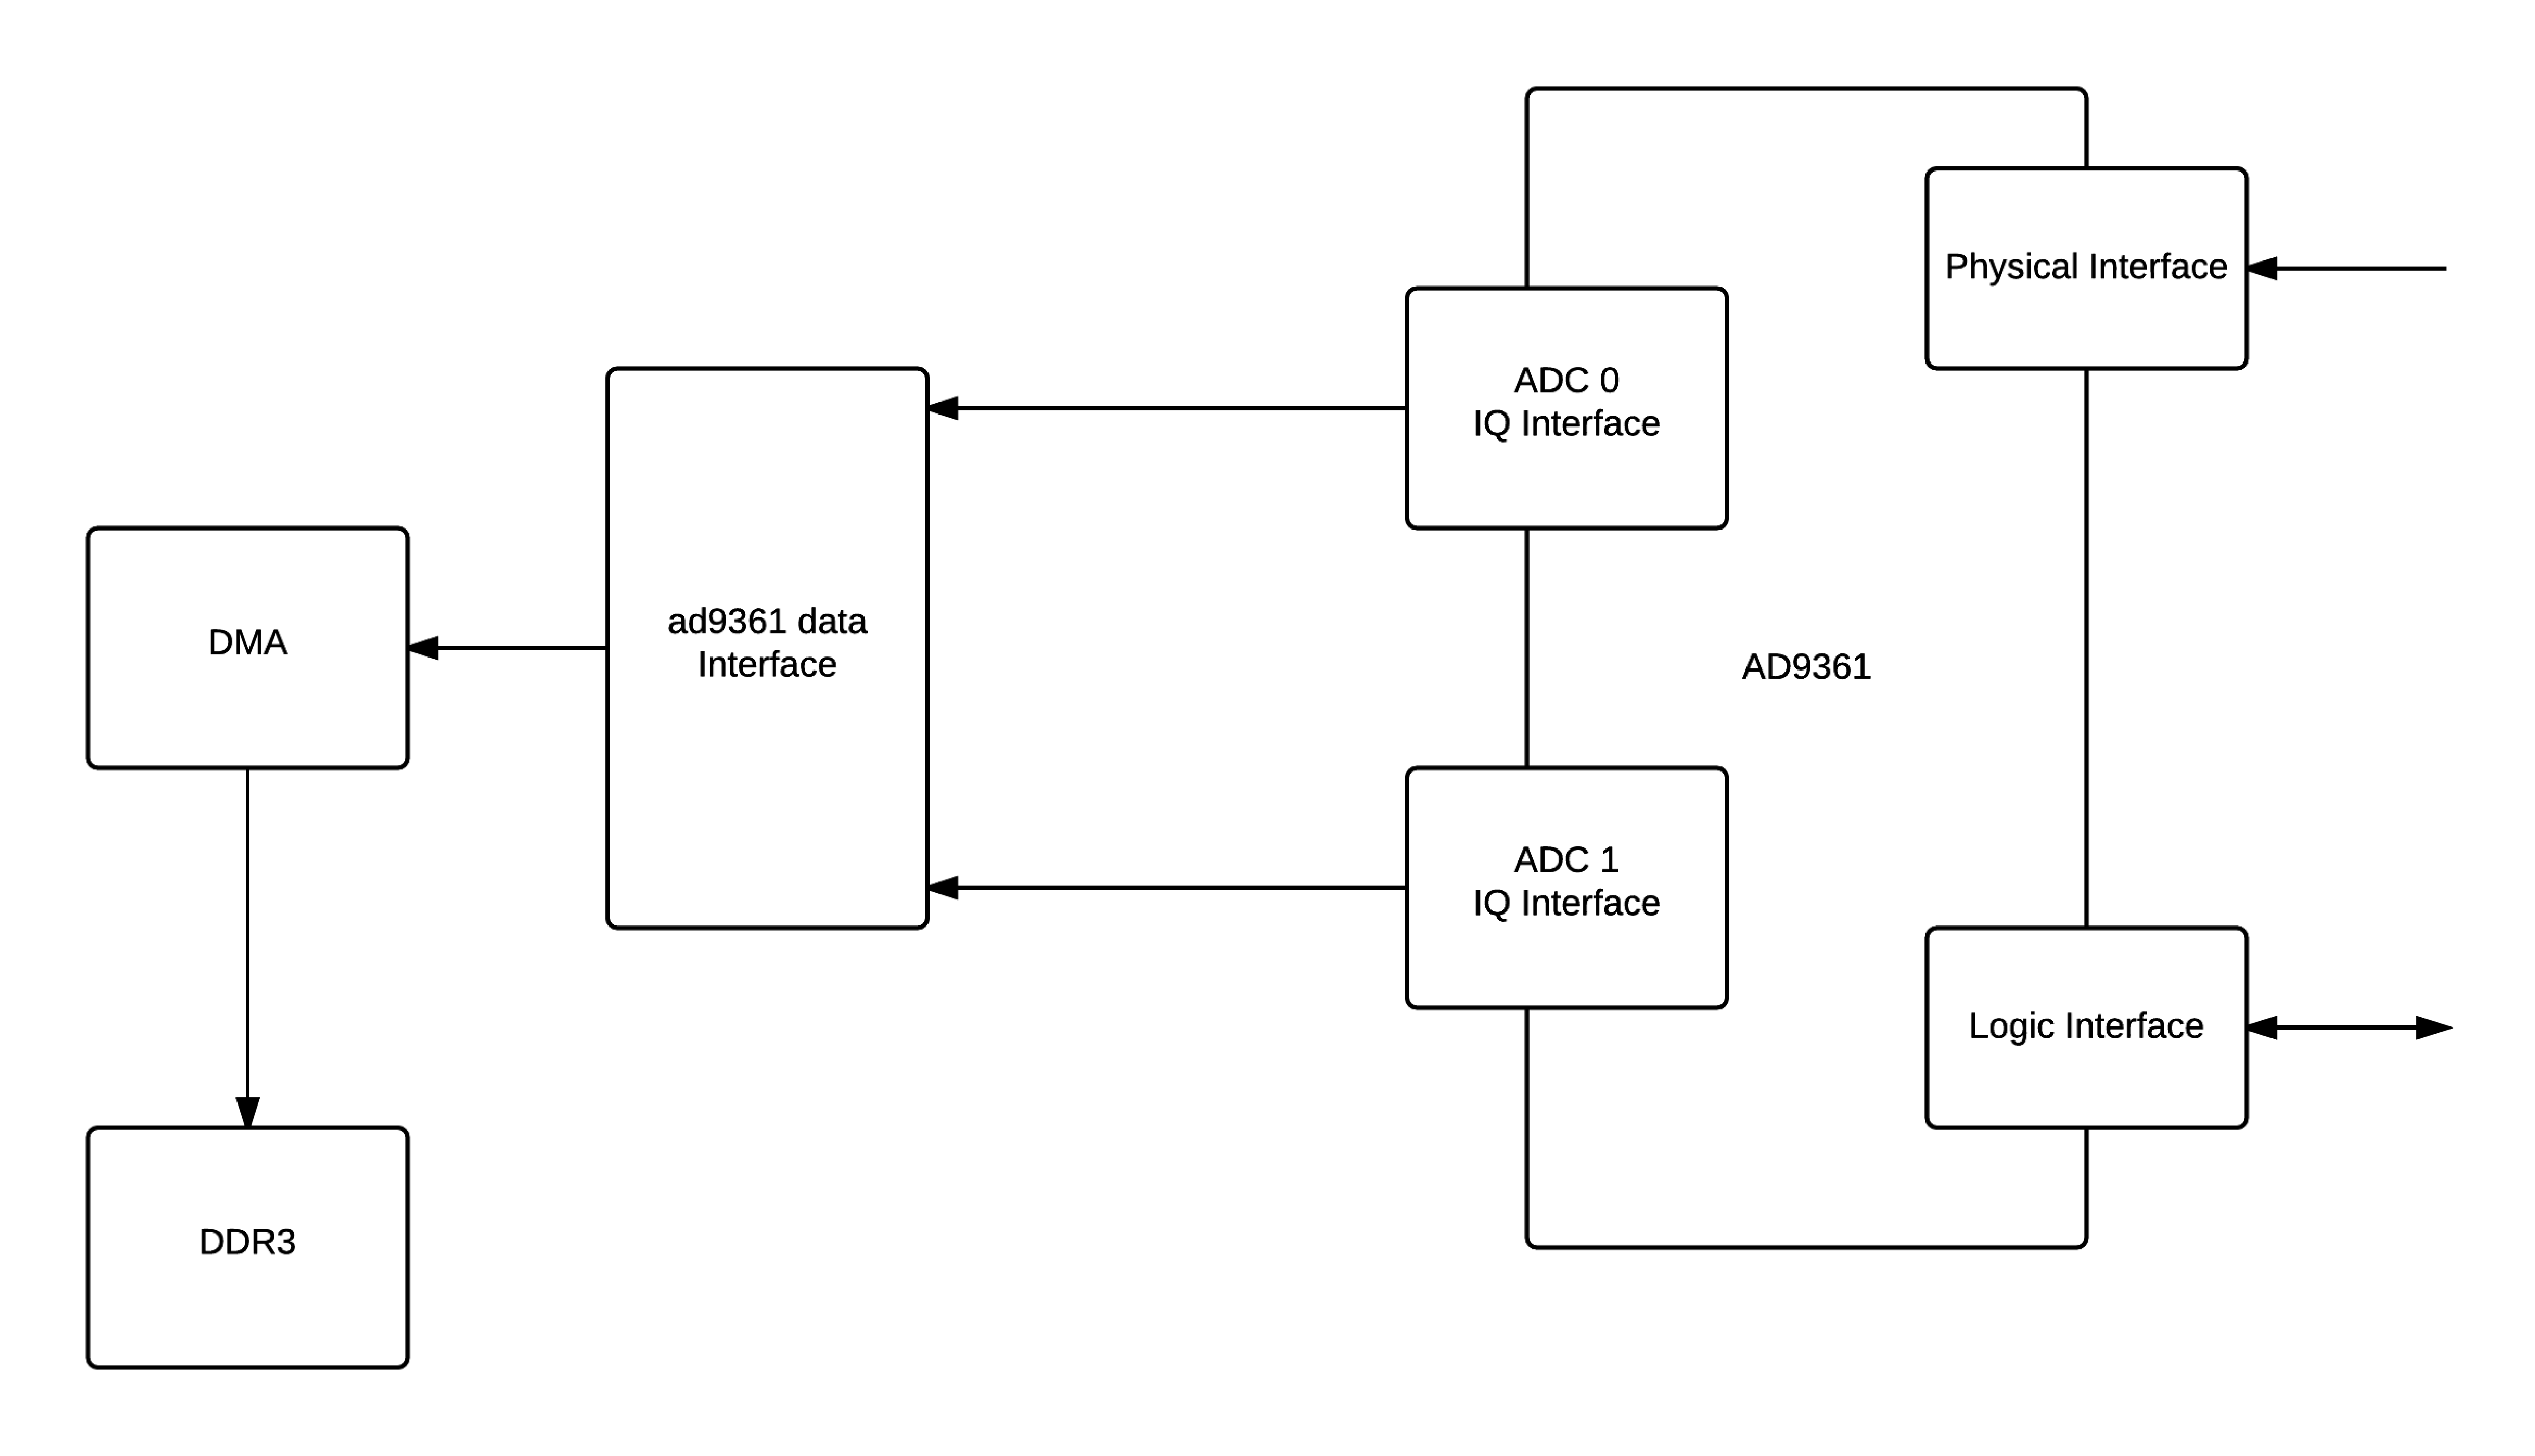
\includegraphics[width=0.65\textwidth]{./figures/adc_dma}
    \caption{ ad9361 ADC interface with DMA
    \label{fig:ad9361rxdma}}
\end{figure}


\subsection{Data Interface}

The data interface from the ad9361 to the FPGA logic is implemented as an IP in
the FPGA design and is composed by two parts, a transmitting interface and a
receiving interface. The transmitting interface connects the DMA, which is
reading data from the main memory, with the DAC interface and the receiving
interface connects the ADC output with the DMA that writes on the main memory,
in the subsections below the two interface will be more explored.

%ad9361_data interface image
\begin{figure}[htbp]
    \centering
    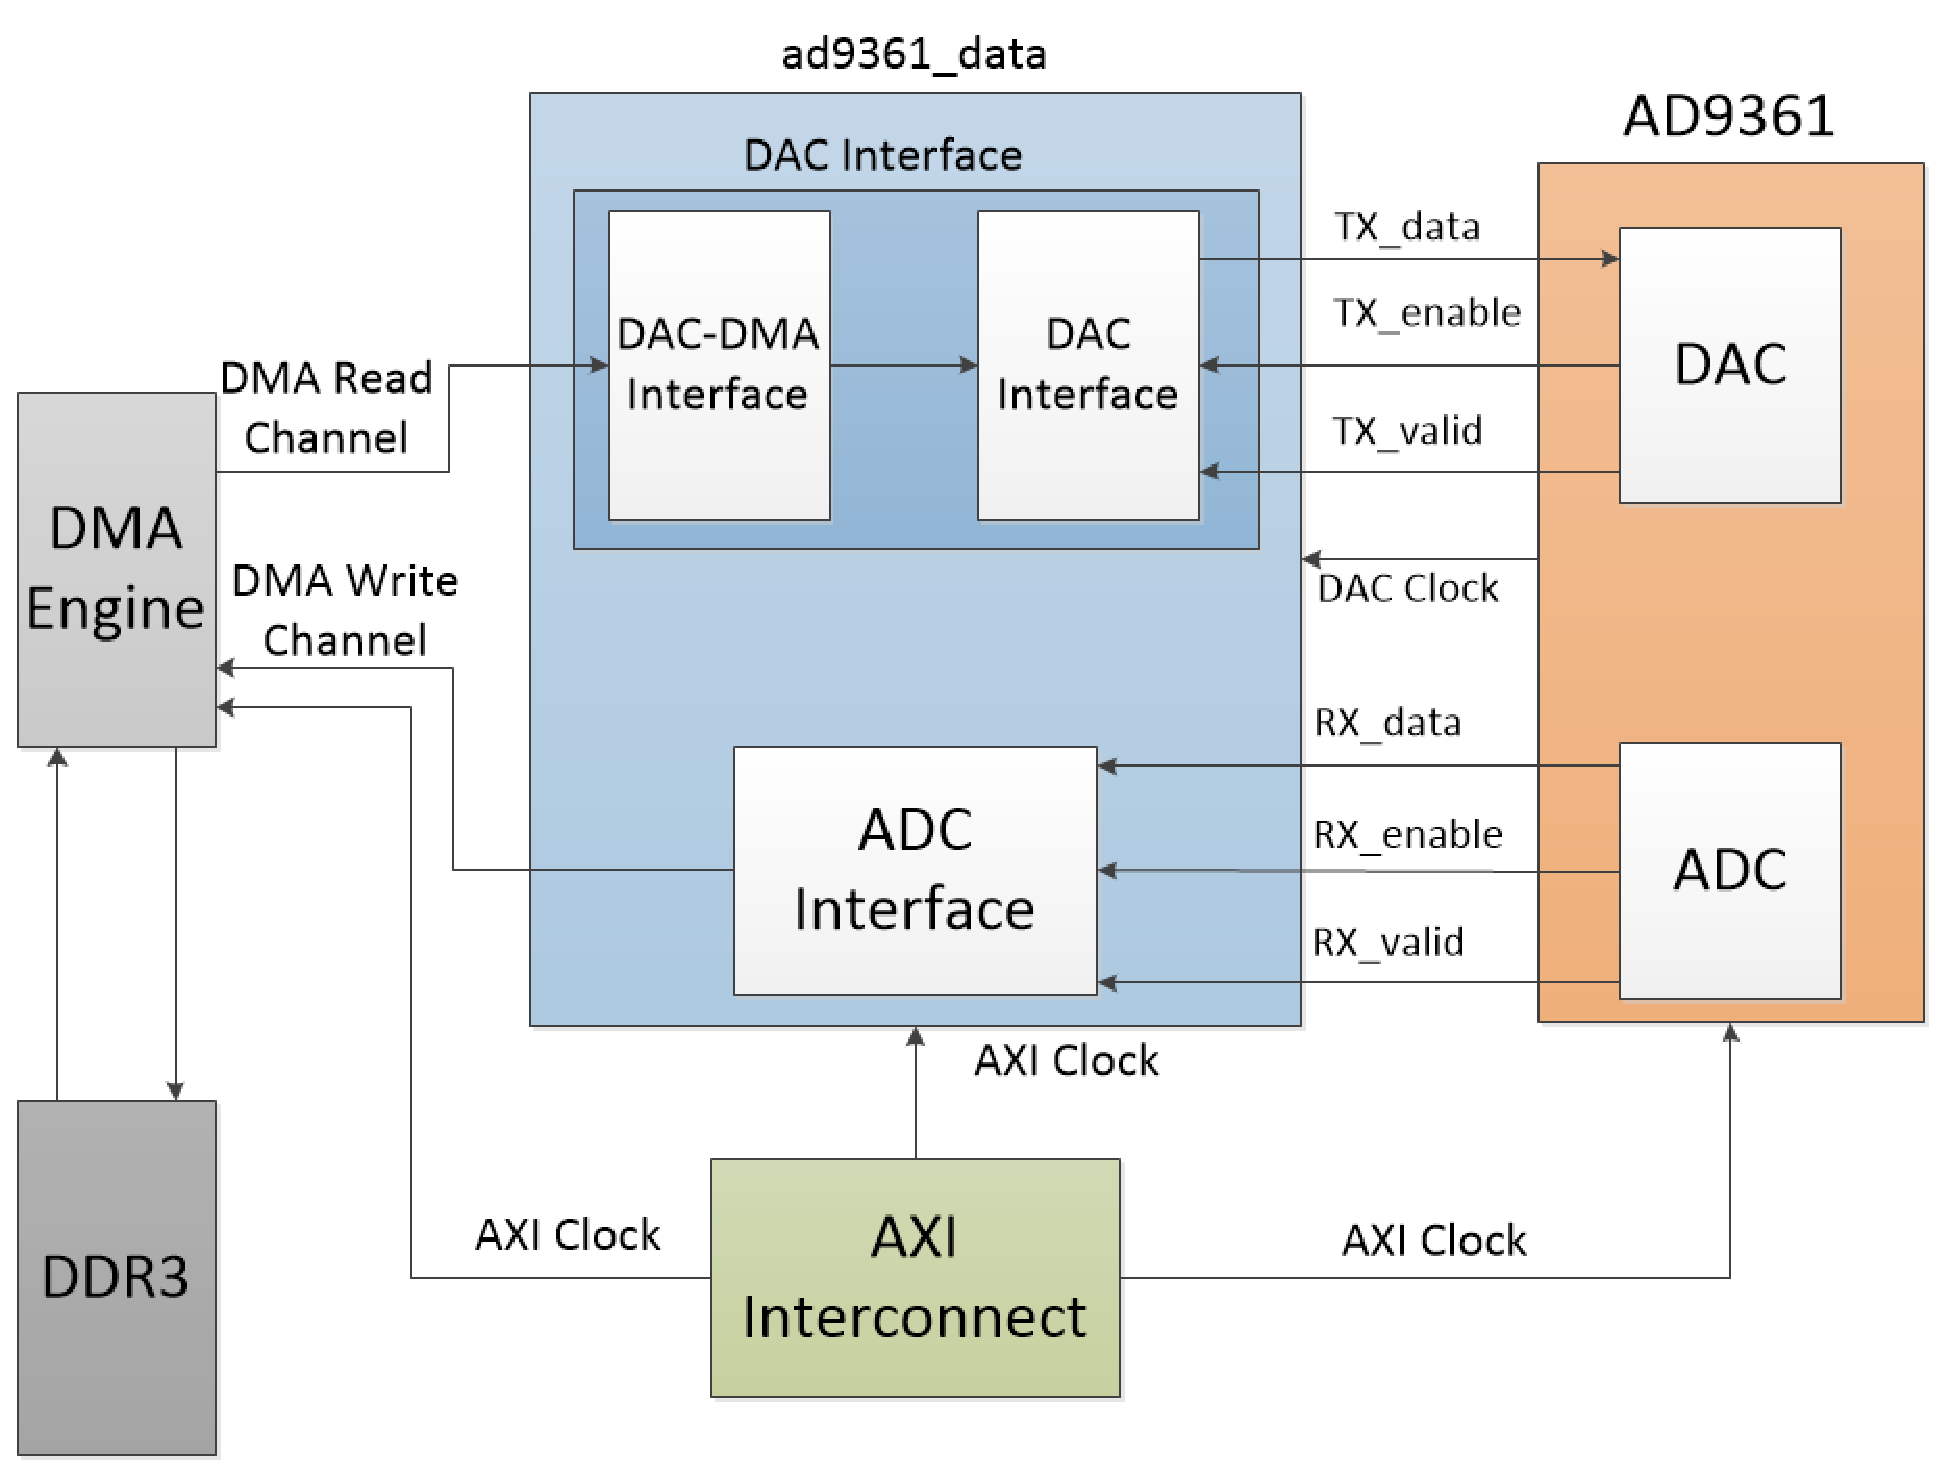
\includegraphics[width=0.65\textwidth]{./figures/data_if}
    \caption{ AD9361 Data Interface Block Diagram
    \label{fig:databd}}
\end{figure}

\subsubsection{Transmitting Interface (Tx)}

The receiving interface itself is divided in two main blocks, one block being the
DAC-DMA interface and the other is the DAC interface. The DAC-DMA interface controls
the reading channel of the DMA block, creating a “bottleneck” based on the reading
clock, thus the DMA reading is limited by the reading clock, which is a way of
synchronizing the DMA reading by the DAC clock, it does not work in perfectly but
is a better solution than simply use FIFOs.

The DAC-DMA is implemented using a commuter controlling a demultiplexer block,
this means that the data read from the memory by the DMA is loaded one into the
demultiplexer and it feeds one channel at the time, both channels are enabled
for use

Below it is possible to see a block diagram of the interface:

\begin{figure}[htbp]
    \centering
    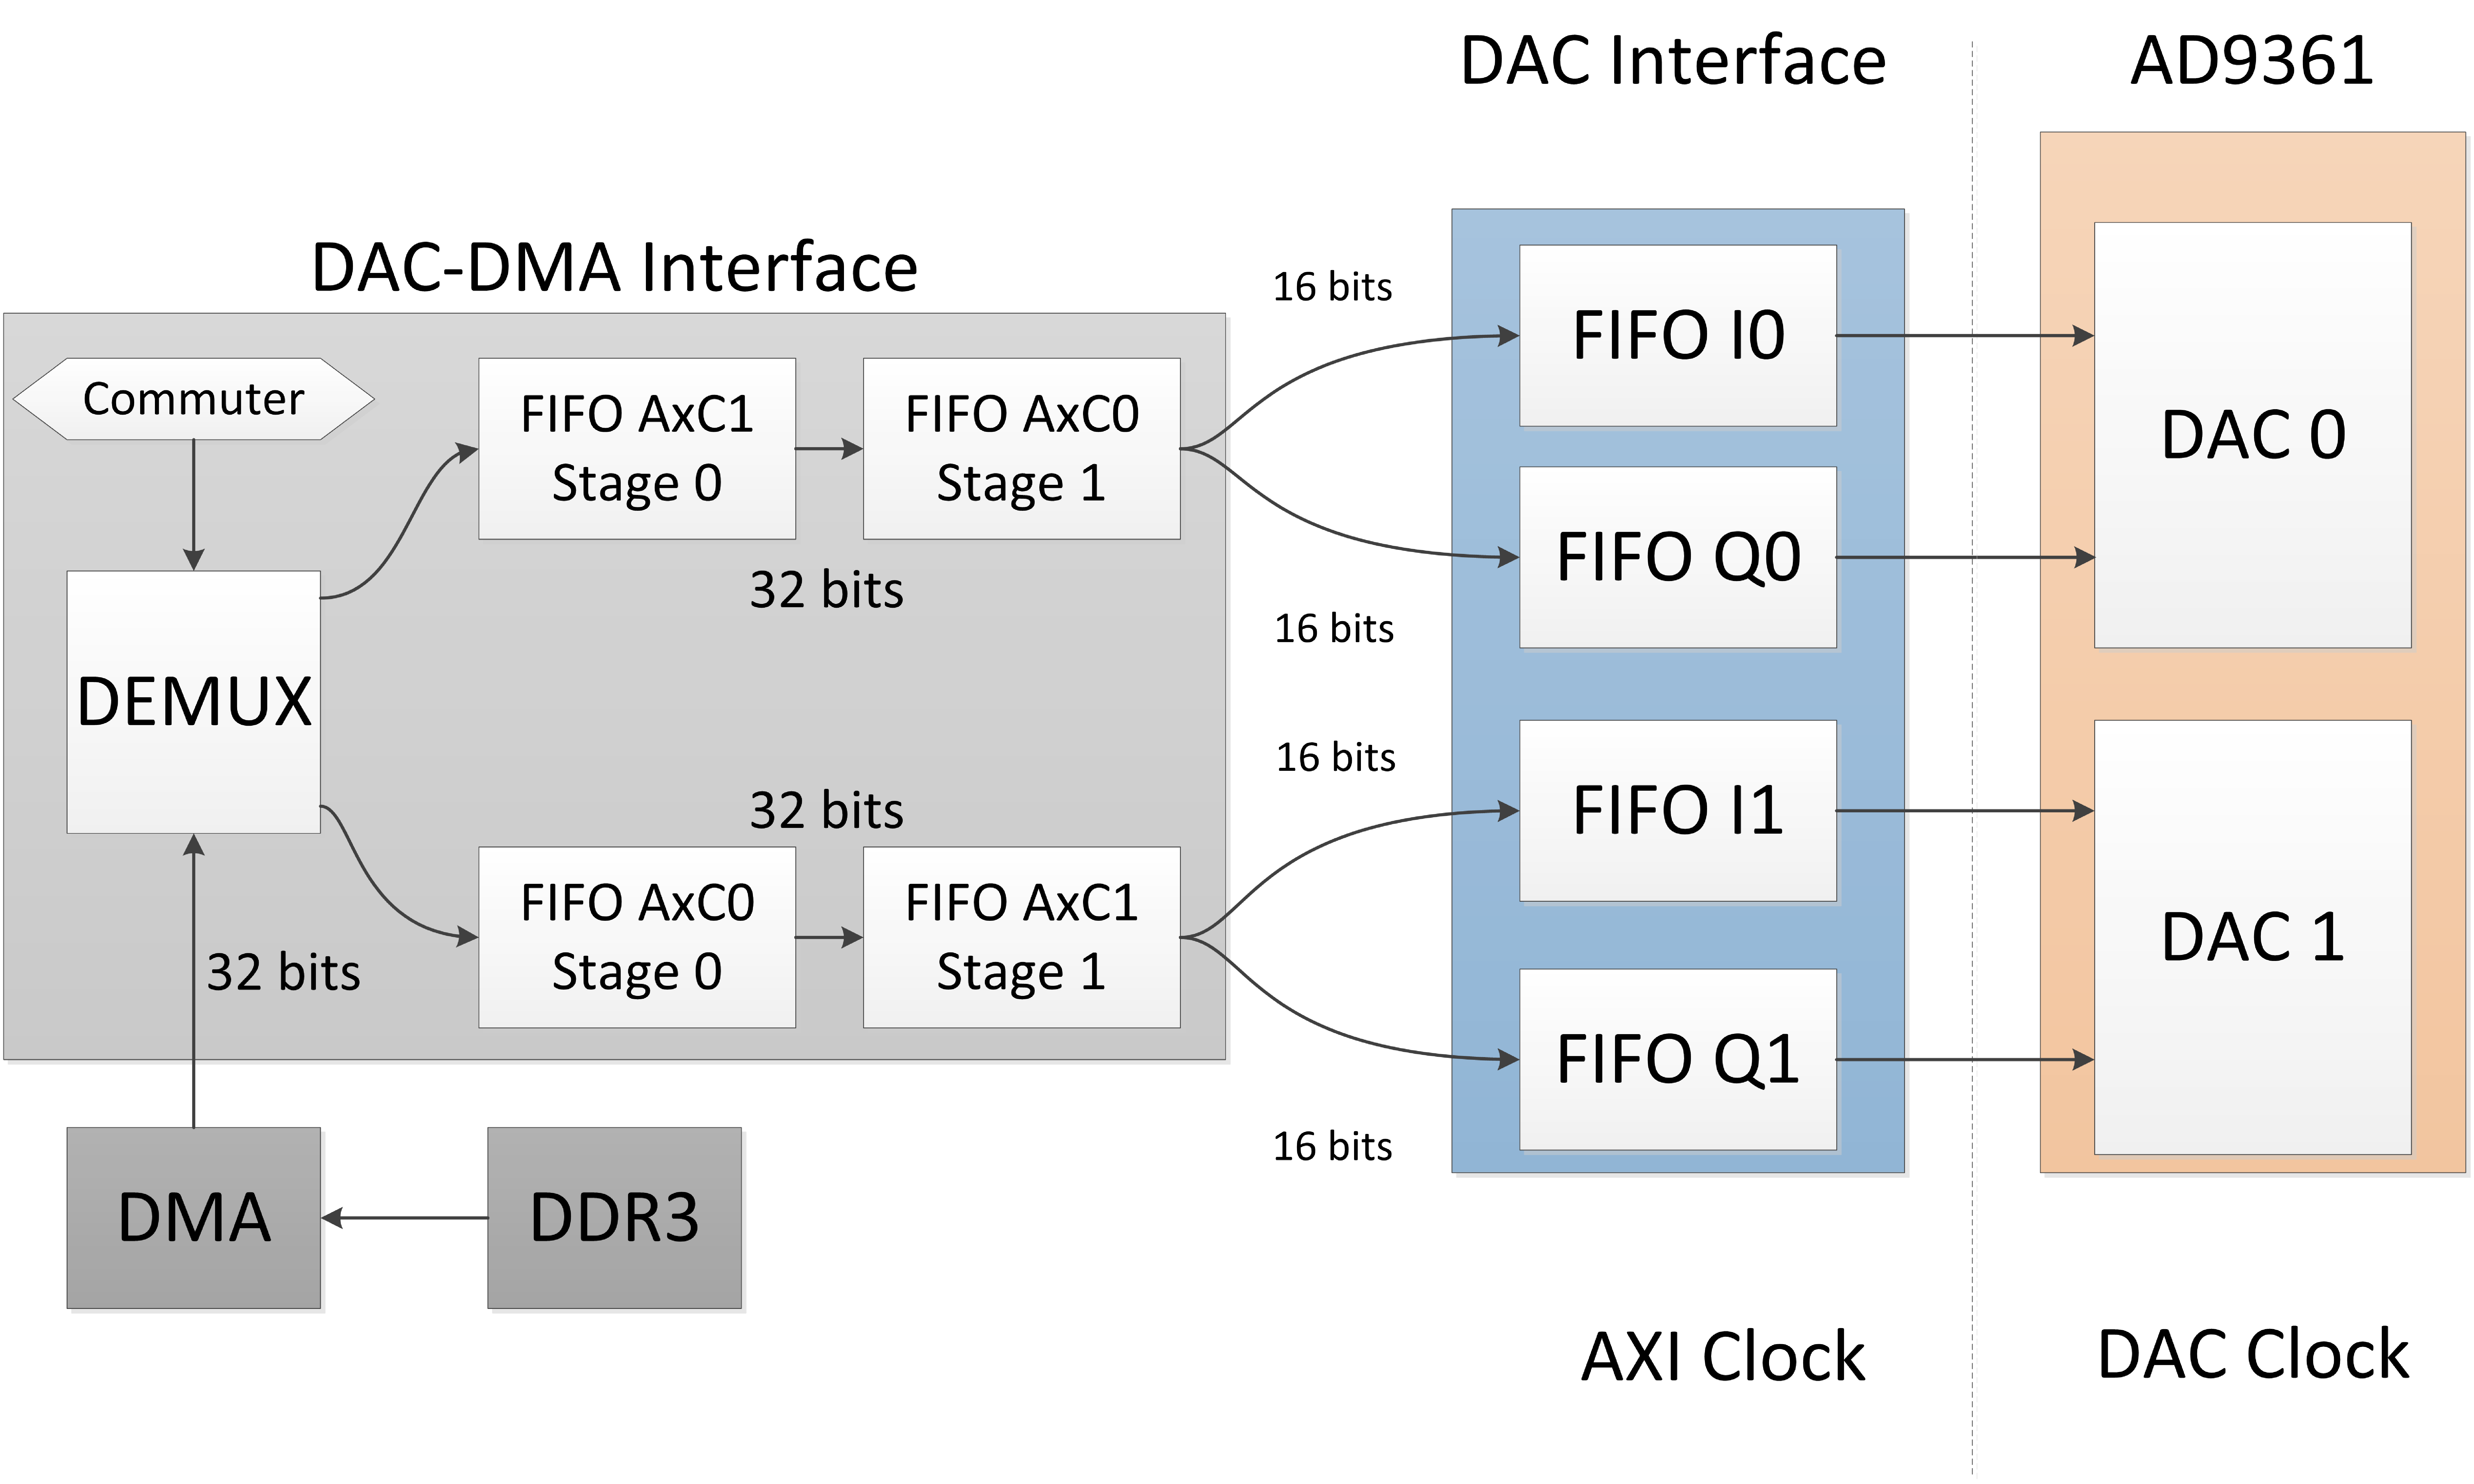
\includegraphics[width=0.65\textwidth]{./figures/txdata_if}
    \caption{ Block diagram of the TX part in the data interface
    \label{fig:dataiftx}}
\end{figure}

\subsubsection{Receiving Interface (Rx)}

The receiving interface itself is rather simple in comparison with the
transmitting interface because the speed in which the data is read by the DMA is
already limited by the DAC clock from the ad9361 interface, thus the ADC
interface has just to commute both channels into one, feeding one sample from
each ADC channel at a time to the DMA, be able to accomplish such, there is a
state machine to control the fifo output to the DMA as can be seen in figure
\ref{fig:dataifrx}.

Below it is possible to see a block diagram describing the Receiving interface with
more details:

\begin{figure}[htbp]
    \centering
    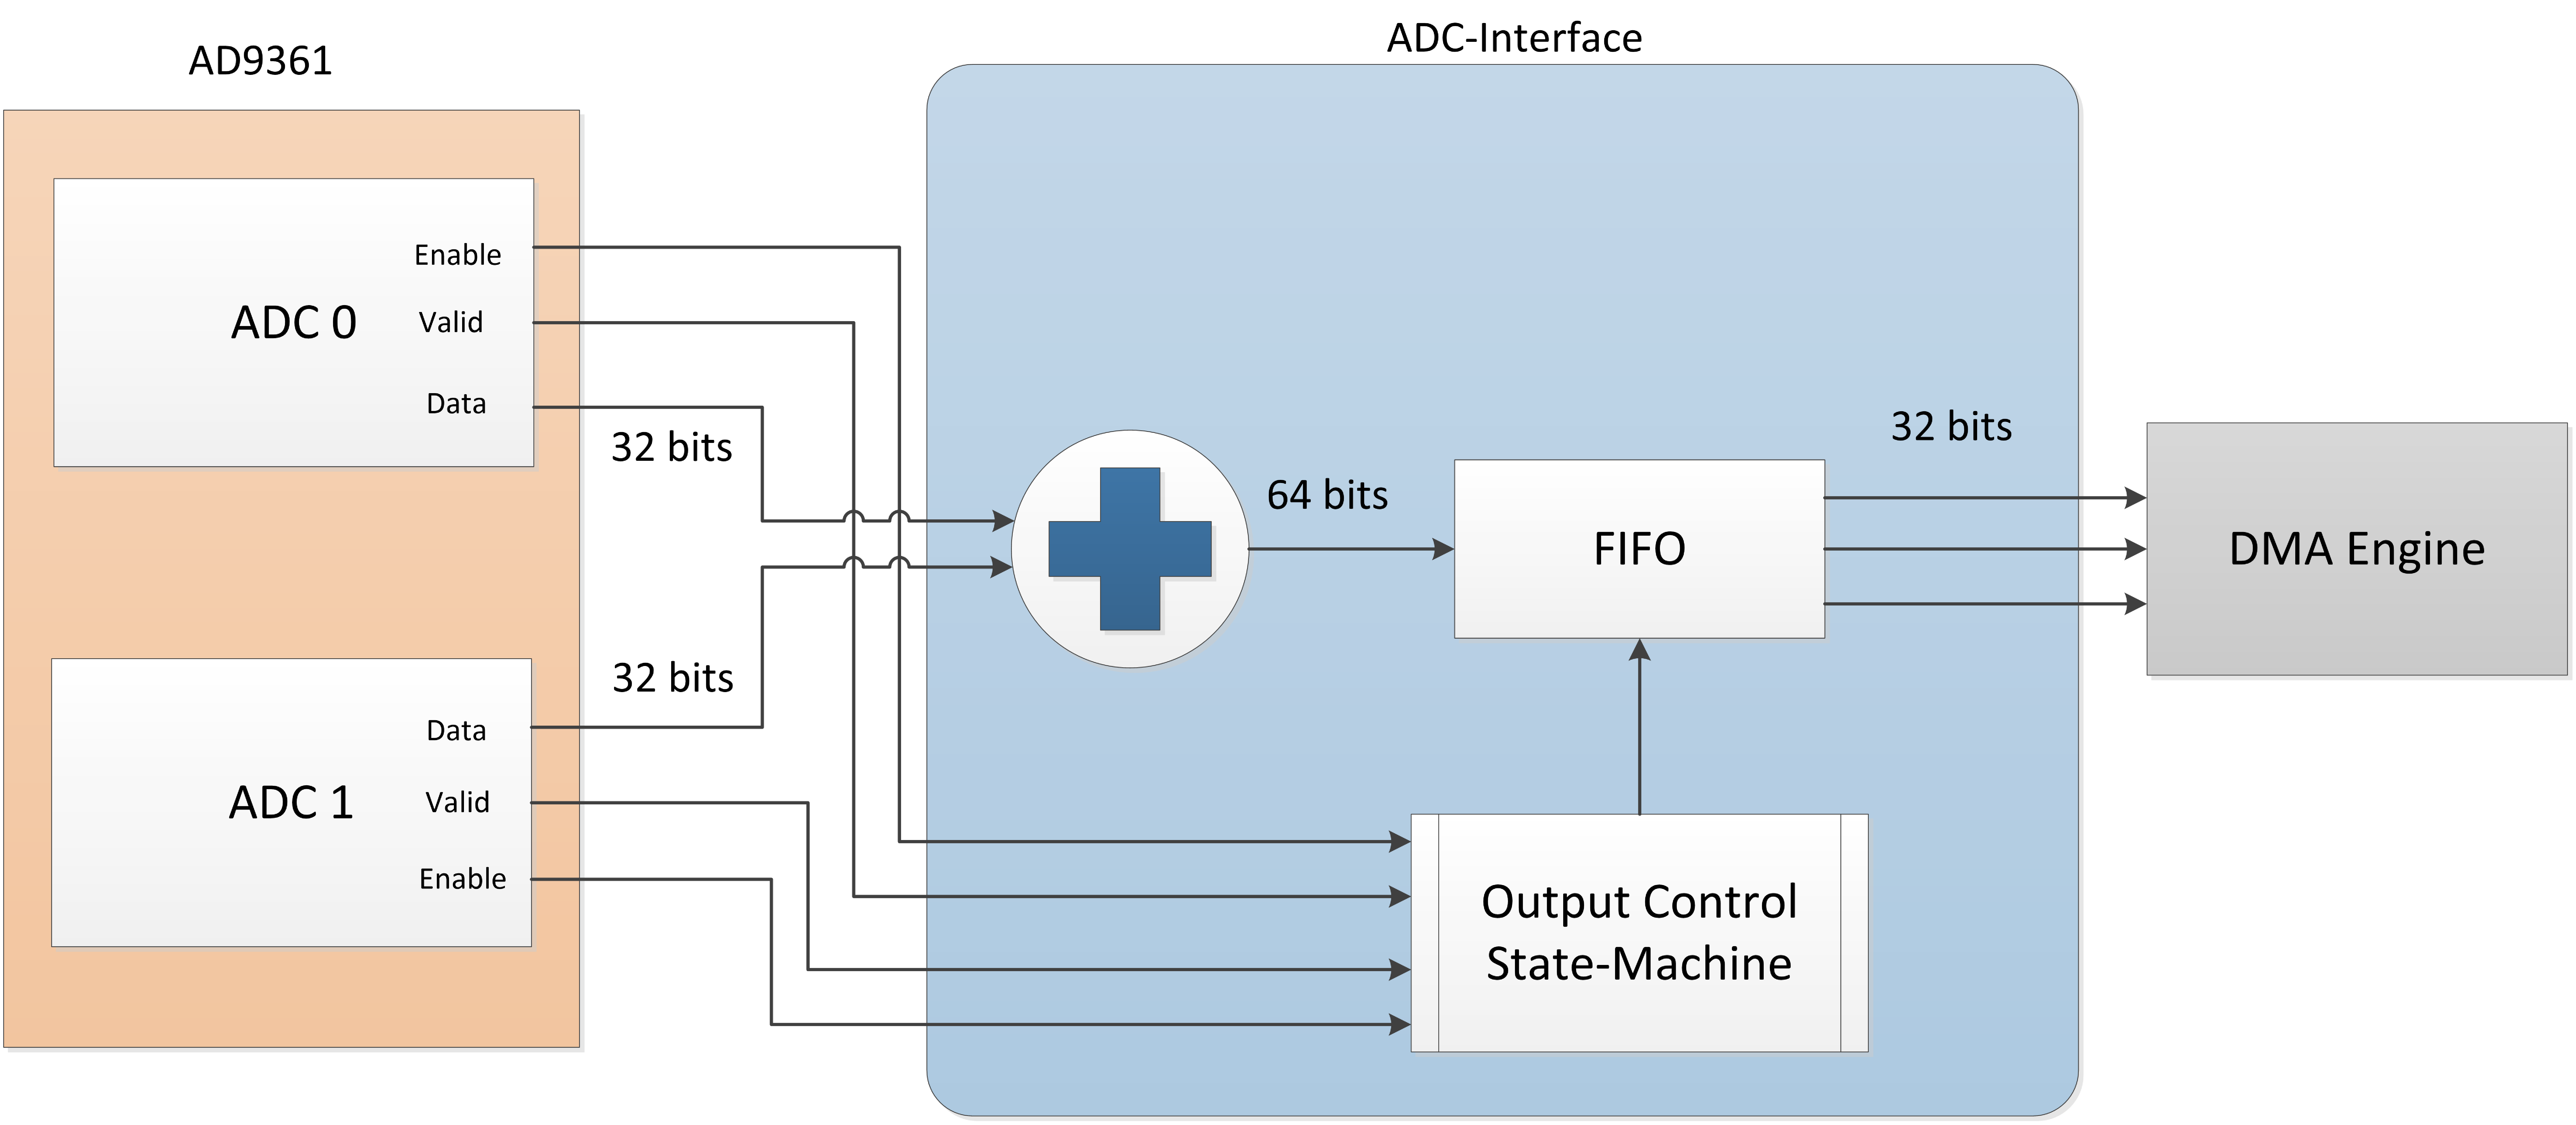
\includegraphics[width=0.65\textwidth]{./figures/rxdata_if}
    \caption{ Block diagram of the RX part in the data interface
    \label{fig:dataifrx}}
\end{figure}

\section{Driver}
\label{impl:driver}

This setup driver has several parts, it not only initiates the FMComms2 hardware
but also initiates all the systems in the FPGA design, like Interrupt Controller,
 DMA, SPI and GPIO needed to control and read/write data into the FMComms2.

The hardware drivers itself are not extremely complicated nor needed to be changed
too much, Xilinx offers all the basic drivers for the boards, for example, DMA Engine,
Ethernet PHY and Interrupt System, the only thing which must be handled with care is
the address space and device ID for each block, knowing how the IP is configured,
or which option he is configured to run is the key to make a driver work.

Xilinx also packs the design tools with documented examples, one for each running
configuration of the device, of course there are always unpredictable things to come,
however there is full support for debugging the program inside the soft processor
Microblaze.

\subsection{AD9361 Driver}

The ad9361 driver is very complex and carries the job of initializing and
configuring the FMcomms2 chip, it also initializes the GPIO and SPI drivers,
which functionality are not worth to explain deeply because they are used for
control and communication and there was no need to modify or to add any
functions to those, their role on the ad9361 is explained in the subsection
\ref{subsec:fmcomms2}.

The initialization begins writing in all the ad9361 registers with the
initialization parameters, in the appendix X there is the explanation of some of
these parameters  and after this, the driver initializes all the PLLs and begin
to calibrate the analog and digital interfaces. With the ad9361 initialization
complete it is possible to change parameters, reconfigure filters and  change
oscillators frequency, if any parameter such as this is changed, the driver must
be recalibrate, however it is done automatically.The process of initialization,
and configuration for this work is explained in the figure \ref{fig:ad9361init}.

%adicionar diagrama de fluxo da inicialização do ad9361

\begin{figure}[htbp]
    \centering
    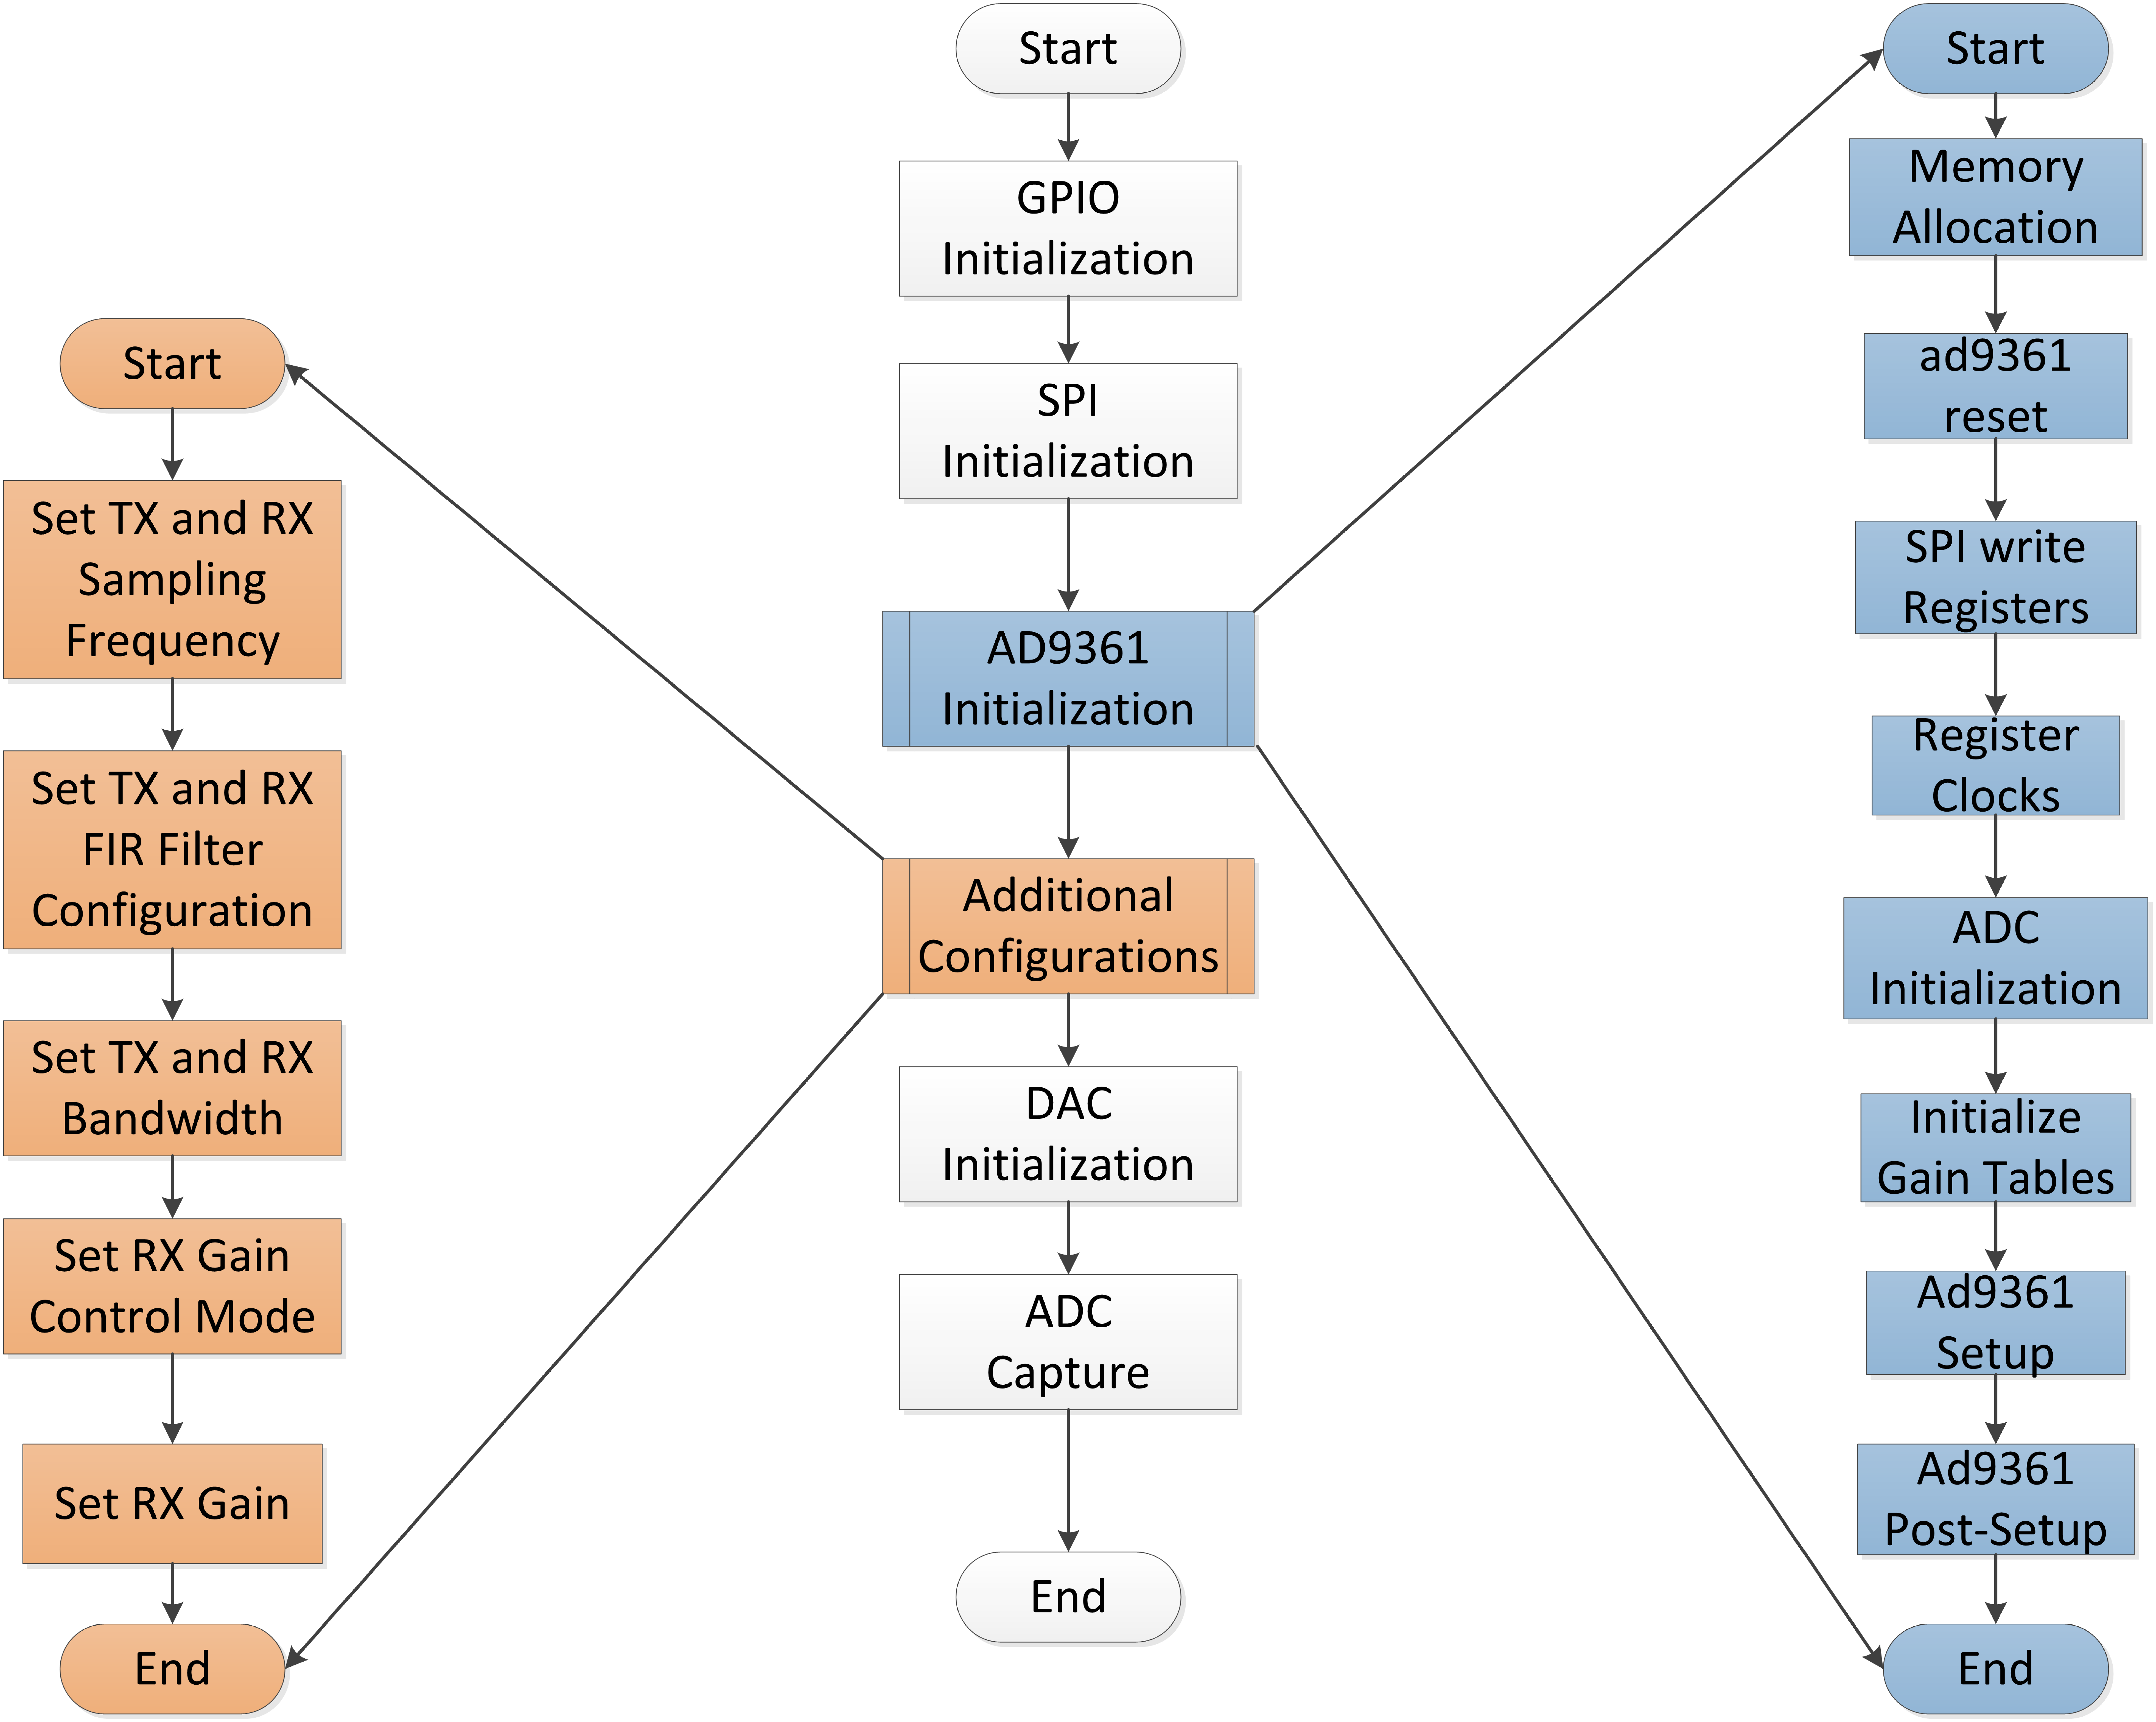
\includegraphics[width=0.75\textwidth]{./figures/ad9361_driver}
    \caption{ AD9361 initialization diagram
    \label{fig:ad9361init}}
\end{figure}

\subsection{Interrupts and DMA}

Basically both Ethernet and FMComms2 utilizes the DMA Engine to read and write in
the DDR3 Memory and thus DMA Engine uses interrupt to inform the processor regarding
the data read and write. So basically the DMA has to initialize the configuration,
and then configure the device.

After device is configured, since the DMA is configured in scatter gather mode,
there is the need to allocate the Block Descriptors for Transmitting (reading)
and Receiving (writing), each block descriptor carries a the beginning address
of the memory to be read, the size of the reading operation and the address of
the next block to read, basically this allows for the DMA to read non continuous
memory spaces.

After all the blocks are processed by DMA and all the reading is done, the DMA
generates an interrupt to inform the processor that the reading process is done
and in such interrupt routine the cyclic process is implemented, it basically
sends DMA back to the start Block descriptor and the process of reading the
memory runs again and again until the kill signal is asserted, this is not the
optimal solution, however it is the one which worked for now.

In the normal mode, the DMA expects and address and a size, and the it begins
reading or writing in this address until the end of the size and the the DMA
asserts interrupt and stops which is not convenient for this work.

The initialization steps for both DMA and INTC are described in the figure
\ref{fig:intcdmainit}.

\begin{figure}[htbp]
    \centering
    
\includegraphics[width=0.85\textwidth]{./figures/dma_intc_driver}
    \caption{ Interrupts and DMA execution diagram
    \label{fig:intcdmainit}}
\end{figure}

\section{Applications}

This setup was meant to be used in the academic and research and development
environments for such it is extensively documented in this document and in the
source codes in the repository, thus this section aims to be a guideline for
whoever needs to use this work for research or study.

\subsection{Academic Environment}

This setup was meant to be used in such academic environment, the data and control
interface are ready to be used, for this the student can generate the data in
matlab and load it as a vector in a .h file, this file shall be read by the DMA
driver.
There is also the possibility to develop a modulation/demodulation block
and input this block feeding the data interface, thus all the modulated data can
be transmitted and received, the only limitation of such development would be the
FPGA board own DSP capability.

\subsection{Research environment}

In the research and development environment, this work can be used as a testbed
for any algorithm in LTE frequency range like compression, synchronization and
transmission tests. This setup saves time in the development where the developer
does not need to worry about any hardware issues and focus on the algorithm.
